
% Default to the notebook output style

    


% Inherit from the specified cell style.




    
\documentclass[11pt]{article}

    
    
    \usepackage[T1]{fontenc}
    % Nicer default font (+ math font) than Computer Modern for most use cases
    \usepackage{mathpazo}

    % Basic figure setup, for now with no caption control since it's done
    % automatically by Pandoc (which extracts ![](path) syntax from Markdown).
    \usepackage{graphicx}
    % We will generate all images so they have a width \maxwidth. This means
    % that they will get their normal width if they fit onto the page, but
    % are scaled down if they would overflow the margins.
    \makeatletter
    \def\maxwidth{\ifdim\Gin@nat@width>\linewidth\linewidth
    \else\Gin@nat@width\fi}
    \makeatother
    \let\Oldincludegraphics\includegraphics
    % Set max figure width to be 80% of text width, for now hardcoded.
    \renewcommand{\includegraphics}[1]{\Oldincludegraphics[width=.8\maxwidth]{#1}}
    % Ensure that by default, figures have no caption (until we provide a
    % proper Figure object with a Caption API and a way to capture that
    % in the conversion process - todo).
    \usepackage{caption}
    \DeclareCaptionLabelFormat{nolabel}{}
    \captionsetup{labelformat=nolabel}

    \usepackage{adjustbox} % Used to constrain images to a maximum size 
    \usepackage{xcolor} % Allow colors to be defined
    \usepackage{enumerate} % Needed for markdown enumerations to work
    \usepackage{geometry} % Used to adjust the document margins
    \usepackage{amsmath} % Equations
    \usepackage{amssymb} % Equations
    \usepackage{textcomp} % defines textquotesingle
    % Hack from http://tex.stackexchange.com/a/47451/13684:
    \AtBeginDocument{%
        \def\PYZsq{\textquotesingle}% Upright quotes in Pygmentized code
    }
    \usepackage{upquote} % Upright quotes for verbatim code
    \usepackage{eurosym} % defines \euro
    \usepackage[mathletters]{ucs} % Extended unicode (utf-8) support
    \usepackage[utf8x]{inputenc} % Allow utf-8 characters in the tex document
    \usepackage{fancyvrb} % verbatim replacement that allows latex
    \usepackage{grffile} % extends the file name processing of package graphics 
                         % to support a larger range 
    % The hyperref package gives us a pdf with properly built
    % internal navigation ('pdf bookmarks' for the table of contents,
    % internal cross-reference links, web links for URLs, etc.)
    \usepackage{hyperref}
    \usepackage{longtable} % longtable support required by pandoc >1.10
    \usepackage{booktabs}  % table support for pandoc > 1.12.2
    \usepackage[inline]{enumitem} % IRkernel/repr support (it uses the enumerate* environment)
    \usepackage[normalem]{ulem} % ulem is needed to support strikethroughs (\sout)
                                % normalem makes italics be italics, not underlines
    

    
    
    % Colors for the hyperref package
    \definecolor{urlcolor}{rgb}{0,.145,.698}
    \definecolor{linkcolor}{rgb}{.71,0.21,0.01}
    \definecolor{citecolor}{rgb}{.12,.54,.11}

    % ANSI colors
    \definecolor{ansi-black}{HTML}{3E424D}
    \definecolor{ansi-black-intense}{HTML}{282C36}
    \definecolor{ansi-red}{HTML}{E75C58}
    \definecolor{ansi-red-intense}{HTML}{B22B31}
    \definecolor{ansi-green}{HTML}{00A250}
    \definecolor{ansi-green-intense}{HTML}{007427}
    \definecolor{ansi-yellow}{HTML}{DDB62B}
    \definecolor{ansi-yellow-intense}{HTML}{B27D12}
    \definecolor{ansi-blue}{HTML}{208FFB}
    \definecolor{ansi-blue-intense}{HTML}{0065CA}
    \definecolor{ansi-magenta}{HTML}{D160C4}
    \definecolor{ansi-magenta-intense}{HTML}{A03196}
    \definecolor{ansi-cyan}{HTML}{60C6C8}
    \definecolor{ansi-cyan-intense}{HTML}{258F8F}
    \definecolor{ansi-white}{HTML}{C5C1B4}
    \definecolor{ansi-white-intense}{HTML}{A1A6B2}

    % commands and environments needed by pandoc snippets
    % extracted from the output of `pandoc -s`
    \providecommand{\tightlist}{%
      \setlength{\itemsep}{0pt}\setlength{\parskip}{0pt}}
    \DefineVerbatimEnvironment{Highlighting}{Verbatim}{commandchars=\\\{\}}
    % Add ',fontsize=\small' for more characters per line
    \newenvironment{Shaded}{}{}
    \newcommand{\KeywordTok}[1]{\textcolor[rgb]{0.00,0.44,0.13}{\textbf{{#1}}}}
    \newcommand{\DataTypeTok}[1]{\textcolor[rgb]{0.56,0.13,0.00}{{#1}}}
    \newcommand{\DecValTok}[1]{\textcolor[rgb]{0.25,0.63,0.44}{{#1}}}
    \newcommand{\BaseNTok}[1]{\textcolor[rgb]{0.25,0.63,0.44}{{#1}}}
    \newcommand{\FloatTok}[1]{\textcolor[rgb]{0.25,0.63,0.44}{{#1}}}
    \newcommand{\CharTok}[1]{\textcolor[rgb]{0.25,0.44,0.63}{{#1}}}
    \newcommand{\StringTok}[1]{\textcolor[rgb]{0.25,0.44,0.63}{{#1}}}
    \newcommand{\CommentTok}[1]{\textcolor[rgb]{0.38,0.63,0.69}{\textit{{#1}}}}
    \newcommand{\OtherTok}[1]{\textcolor[rgb]{0.00,0.44,0.13}{{#1}}}
    \newcommand{\AlertTok}[1]{\textcolor[rgb]{1.00,0.00,0.00}{\textbf{{#1}}}}
    \newcommand{\FunctionTok}[1]{\textcolor[rgb]{0.02,0.16,0.49}{{#1}}}
    \newcommand{\RegionMarkerTok}[1]{{#1}}
    \newcommand{\ErrorTok}[1]{\textcolor[rgb]{1.00,0.00,0.00}{\textbf{{#1}}}}
    \newcommand{\NormalTok}[1]{{#1}}
    
    % Additional commands for more recent versions of Pandoc
    \newcommand{\ConstantTok}[1]{\textcolor[rgb]{0.53,0.00,0.00}{{#1}}}
    \newcommand{\SpecialCharTok}[1]{\textcolor[rgb]{0.25,0.44,0.63}{{#1}}}
    \newcommand{\VerbatimStringTok}[1]{\textcolor[rgb]{0.25,0.44,0.63}{{#1}}}
    \newcommand{\SpecialStringTok}[1]{\textcolor[rgb]{0.73,0.40,0.53}{{#1}}}
    \newcommand{\ImportTok}[1]{{#1}}
    \newcommand{\DocumentationTok}[1]{\textcolor[rgb]{0.73,0.13,0.13}{\textit{{#1}}}}
    \newcommand{\AnnotationTok}[1]{\textcolor[rgb]{0.38,0.63,0.69}{\textbf{\textit{{#1}}}}}
    \newcommand{\CommentVarTok}[1]{\textcolor[rgb]{0.38,0.63,0.69}{\textbf{\textit{{#1}}}}}
    \newcommand{\VariableTok}[1]{\textcolor[rgb]{0.10,0.09,0.49}{{#1}}}
    \newcommand{\ControlFlowTok}[1]{\textcolor[rgb]{0.00,0.44,0.13}{\textbf{{#1}}}}
    \newcommand{\OperatorTok}[1]{\textcolor[rgb]{0.40,0.40,0.40}{{#1}}}
    \newcommand{\BuiltInTok}[1]{{#1}}
    \newcommand{\ExtensionTok}[1]{{#1}}
    \newcommand{\PreprocessorTok}[1]{\textcolor[rgb]{0.74,0.48,0.00}{{#1}}}
    \newcommand{\AttributeTok}[1]{\textcolor[rgb]{0.49,0.56,0.16}{{#1}}}
    \newcommand{\InformationTok}[1]{\textcolor[rgb]{0.38,0.63,0.69}{\textbf{\textit{{#1}}}}}
    \newcommand{\WarningTok}[1]{\textcolor[rgb]{0.38,0.63,0.69}{\textbf{\textit{{#1}}}}}
    
    
    % Define a nice break command that doesn't care if a line doesn't already
    % exist.
    \def\br{\hspace*{\fill} \\* }
    % Math Jax compatability definitions
    \def\gt{>}
    \def\lt{<}
    % Document parameters
    \title{Near Final Draft}
    
    
    

    % Pygments definitions
    
\makeatletter
\def\PY@reset{\let\PY@it=\relax \let\PY@bf=\relax%
    \let\PY@ul=\relax \let\PY@tc=\relax%
    \let\PY@bc=\relax \let\PY@ff=\relax}
\def\PY@tok#1{\csname PY@tok@#1\endcsname}
\def\PY@toks#1+{\ifx\relax#1\empty\else%
    \PY@tok{#1}\expandafter\PY@toks\fi}
\def\PY@do#1{\PY@bc{\PY@tc{\PY@ul{%
    \PY@it{\PY@bf{\PY@ff{#1}}}}}}}
\def\PY#1#2{\PY@reset\PY@toks#1+\relax+\PY@do{#2}}

\expandafter\def\csname PY@tok@w\endcsname{\def\PY@tc##1{\textcolor[rgb]{0.73,0.73,0.73}{##1}}}
\expandafter\def\csname PY@tok@c\endcsname{\let\PY@it=\textit\def\PY@tc##1{\textcolor[rgb]{0.25,0.50,0.50}{##1}}}
\expandafter\def\csname PY@tok@cp\endcsname{\def\PY@tc##1{\textcolor[rgb]{0.74,0.48,0.00}{##1}}}
\expandafter\def\csname PY@tok@k\endcsname{\let\PY@bf=\textbf\def\PY@tc##1{\textcolor[rgb]{0.00,0.50,0.00}{##1}}}
\expandafter\def\csname PY@tok@kp\endcsname{\def\PY@tc##1{\textcolor[rgb]{0.00,0.50,0.00}{##1}}}
\expandafter\def\csname PY@tok@kt\endcsname{\def\PY@tc##1{\textcolor[rgb]{0.69,0.00,0.25}{##1}}}
\expandafter\def\csname PY@tok@o\endcsname{\def\PY@tc##1{\textcolor[rgb]{0.40,0.40,0.40}{##1}}}
\expandafter\def\csname PY@tok@ow\endcsname{\let\PY@bf=\textbf\def\PY@tc##1{\textcolor[rgb]{0.67,0.13,1.00}{##1}}}
\expandafter\def\csname PY@tok@nb\endcsname{\def\PY@tc##1{\textcolor[rgb]{0.00,0.50,0.00}{##1}}}
\expandafter\def\csname PY@tok@nf\endcsname{\def\PY@tc##1{\textcolor[rgb]{0.00,0.00,1.00}{##1}}}
\expandafter\def\csname PY@tok@nc\endcsname{\let\PY@bf=\textbf\def\PY@tc##1{\textcolor[rgb]{0.00,0.00,1.00}{##1}}}
\expandafter\def\csname PY@tok@nn\endcsname{\let\PY@bf=\textbf\def\PY@tc##1{\textcolor[rgb]{0.00,0.00,1.00}{##1}}}
\expandafter\def\csname PY@tok@ne\endcsname{\let\PY@bf=\textbf\def\PY@tc##1{\textcolor[rgb]{0.82,0.25,0.23}{##1}}}
\expandafter\def\csname PY@tok@nv\endcsname{\def\PY@tc##1{\textcolor[rgb]{0.10,0.09,0.49}{##1}}}
\expandafter\def\csname PY@tok@no\endcsname{\def\PY@tc##1{\textcolor[rgb]{0.53,0.00,0.00}{##1}}}
\expandafter\def\csname PY@tok@nl\endcsname{\def\PY@tc##1{\textcolor[rgb]{0.63,0.63,0.00}{##1}}}
\expandafter\def\csname PY@tok@ni\endcsname{\let\PY@bf=\textbf\def\PY@tc##1{\textcolor[rgb]{0.60,0.60,0.60}{##1}}}
\expandafter\def\csname PY@tok@na\endcsname{\def\PY@tc##1{\textcolor[rgb]{0.49,0.56,0.16}{##1}}}
\expandafter\def\csname PY@tok@nt\endcsname{\let\PY@bf=\textbf\def\PY@tc##1{\textcolor[rgb]{0.00,0.50,0.00}{##1}}}
\expandafter\def\csname PY@tok@nd\endcsname{\def\PY@tc##1{\textcolor[rgb]{0.67,0.13,1.00}{##1}}}
\expandafter\def\csname PY@tok@s\endcsname{\def\PY@tc##1{\textcolor[rgb]{0.73,0.13,0.13}{##1}}}
\expandafter\def\csname PY@tok@sd\endcsname{\let\PY@it=\textit\def\PY@tc##1{\textcolor[rgb]{0.73,0.13,0.13}{##1}}}
\expandafter\def\csname PY@tok@si\endcsname{\let\PY@bf=\textbf\def\PY@tc##1{\textcolor[rgb]{0.73,0.40,0.53}{##1}}}
\expandafter\def\csname PY@tok@se\endcsname{\let\PY@bf=\textbf\def\PY@tc##1{\textcolor[rgb]{0.73,0.40,0.13}{##1}}}
\expandafter\def\csname PY@tok@sr\endcsname{\def\PY@tc##1{\textcolor[rgb]{0.73,0.40,0.53}{##1}}}
\expandafter\def\csname PY@tok@ss\endcsname{\def\PY@tc##1{\textcolor[rgb]{0.10,0.09,0.49}{##1}}}
\expandafter\def\csname PY@tok@sx\endcsname{\def\PY@tc##1{\textcolor[rgb]{0.00,0.50,0.00}{##1}}}
\expandafter\def\csname PY@tok@m\endcsname{\def\PY@tc##1{\textcolor[rgb]{0.40,0.40,0.40}{##1}}}
\expandafter\def\csname PY@tok@gh\endcsname{\let\PY@bf=\textbf\def\PY@tc##1{\textcolor[rgb]{0.00,0.00,0.50}{##1}}}
\expandafter\def\csname PY@tok@gu\endcsname{\let\PY@bf=\textbf\def\PY@tc##1{\textcolor[rgb]{0.50,0.00,0.50}{##1}}}
\expandafter\def\csname PY@tok@gd\endcsname{\def\PY@tc##1{\textcolor[rgb]{0.63,0.00,0.00}{##1}}}
\expandafter\def\csname PY@tok@gi\endcsname{\def\PY@tc##1{\textcolor[rgb]{0.00,0.63,0.00}{##1}}}
\expandafter\def\csname PY@tok@gr\endcsname{\def\PY@tc##1{\textcolor[rgb]{1.00,0.00,0.00}{##1}}}
\expandafter\def\csname PY@tok@ge\endcsname{\let\PY@it=\textit}
\expandafter\def\csname PY@tok@gs\endcsname{\let\PY@bf=\textbf}
\expandafter\def\csname PY@tok@gp\endcsname{\let\PY@bf=\textbf\def\PY@tc##1{\textcolor[rgb]{0.00,0.00,0.50}{##1}}}
\expandafter\def\csname PY@tok@go\endcsname{\def\PY@tc##1{\textcolor[rgb]{0.53,0.53,0.53}{##1}}}
\expandafter\def\csname PY@tok@gt\endcsname{\def\PY@tc##1{\textcolor[rgb]{0.00,0.27,0.87}{##1}}}
\expandafter\def\csname PY@tok@err\endcsname{\def\PY@bc##1{\setlength{\fboxsep}{0pt}\fcolorbox[rgb]{1.00,0.00,0.00}{1,1,1}{\strut ##1}}}
\expandafter\def\csname PY@tok@kc\endcsname{\let\PY@bf=\textbf\def\PY@tc##1{\textcolor[rgb]{0.00,0.50,0.00}{##1}}}
\expandafter\def\csname PY@tok@kd\endcsname{\let\PY@bf=\textbf\def\PY@tc##1{\textcolor[rgb]{0.00,0.50,0.00}{##1}}}
\expandafter\def\csname PY@tok@kn\endcsname{\let\PY@bf=\textbf\def\PY@tc##1{\textcolor[rgb]{0.00,0.50,0.00}{##1}}}
\expandafter\def\csname PY@tok@kr\endcsname{\let\PY@bf=\textbf\def\PY@tc##1{\textcolor[rgb]{0.00,0.50,0.00}{##1}}}
\expandafter\def\csname PY@tok@bp\endcsname{\def\PY@tc##1{\textcolor[rgb]{0.00,0.50,0.00}{##1}}}
\expandafter\def\csname PY@tok@fm\endcsname{\def\PY@tc##1{\textcolor[rgb]{0.00,0.00,1.00}{##1}}}
\expandafter\def\csname PY@tok@vc\endcsname{\def\PY@tc##1{\textcolor[rgb]{0.10,0.09,0.49}{##1}}}
\expandafter\def\csname PY@tok@vg\endcsname{\def\PY@tc##1{\textcolor[rgb]{0.10,0.09,0.49}{##1}}}
\expandafter\def\csname PY@tok@vi\endcsname{\def\PY@tc##1{\textcolor[rgb]{0.10,0.09,0.49}{##1}}}
\expandafter\def\csname PY@tok@vm\endcsname{\def\PY@tc##1{\textcolor[rgb]{0.10,0.09,0.49}{##1}}}
\expandafter\def\csname PY@tok@sa\endcsname{\def\PY@tc##1{\textcolor[rgb]{0.73,0.13,0.13}{##1}}}
\expandafter\def\csname PY@tok@sb\endcsname{\def\PY@tc##1{\textcolor[rgb]{0.73,0.13,0.13}{##1}}}
\expandafter\def\csname PY@tok@sc\endcsname{\def\PY@tc##1{\textcolor[rgb]{0.73,0.13,0.13}{##1}}}
\expandafter\def\csname PY@tok@dl\endcsname{\def\PY@tc##1{\textcolor[rgb]{0.73,0.13,0.13}{##1}}}
\expandafter\def\csname PY@tok@s2\endcsname{\def\PY@tc##1{\textcolor[rgb]{0.73,0.13,0.13}{##1}}}
\expandafter\def\csname PY@tok@sh\endcsname{\def\PY@tc##1{\textcolor[rgb]{0.73,0.13,0.13}{##1}}}
\expandafter\def\csname PY@tok@s1\endcsname{\def\PY@tc##1{\textcolor[rgb]{0.73,0.13,0.13}{##1}}}
\expandafter\def\csname PY@tok@mb\endcsname{\def\PY@tc##1{\textcolor[rgb]{0.40,0.40,0.40}{##1}}}
\expandafter\def\csname PY@tok@mf\endcsname{\def\PY@tc##1{\textcolor[rgb]{0.40,0.40,0.40}{##1}}}
\expandafter\def\csname PY@tok@mh\endcsname{\def\PY@tc##1{\textcolor[rgb]{0.40,0.40,0.40}{##1}}}
\expandafter\def\csname PY@tok@mi\endcsname{\def\PY@tc##1{\textcolor[rgb]{0.40,0.40,0.40}{##1}}}
\expandafter\def\csname PY@tok@il\endcsname{\def\PY@tc##1{\textcolor[rgb]{0.40,0.40,0.40}{##1}}}
\expandafter\def\csname PY@tok@mo\endcsname{\def\PY@tc##1{\textcolor[rgb]{0.40,0.40,0.40}{##1}}}
\expandafter\def\csname PY@tok@ch\endcsname{\let\PY@it=\textit\def\PY@tc##1{\textcolor[rgb]{0.25,0.50,0.50}{##1}}}
\expandafter\def\csname PY@tok@cm\endcsname{\let\PY@it=\textit\def\PY@tc##1{\textcolor[rgb]{0.25,0.50,0.50}{##1}}}
\expandafter\def\csname PY@tok@cpf\endcsname{\let\PY@it=\textit\def\PY@tc##1{\textcolor[rgb]{0.25,0.50,0.50}{##1}}}
\expandafter\def\csname PY@tok@c1\endcsname{\let\PY@it=\textit\def\PY@tc##1{\textcolor[rgb]{0.25,0.50,0.50}{##1}}}
\expandafter\def\csname PY@tok@cs\endcsname{\let\PY@it=\textit\def\PY@tc##1{\textcolor[rgb]{0.25,0.50,0.50}{##1}}}

\def\PYZbs{\char`\\}
\def\PYZus{\char`\_}
\def\PYZob{\char`\{}
\def\PYZcb{\char`\}}
\def\PYZca{\char`\^}
\def\PYZam{\char`\&}
\def\PYZlt{\char`\<}
\def\PYZgt{\char`\>}
\def\PYZsh{\char`\#}
\def\PYZpc{\char`\%}
\def\PYZdl{\char`\$}
\def\PYZhy{\char`\-}
\def\PYZsq{\char`\'}
\def\PYZdq{\char`\"}
\def\PYZti{\char`\~}
% for compatibility with earlier versions
\def\PYZat{@}
\def\PYZlb{[}
\def\PYZrb{]}
\makeatother


    % Exact colors from NB
    \definecolor{incolor}{rgb}{0.0, 0.0, 0.5}
    \definecolor{outcolor}{rgb}{0.545, 0.0, 0.0}



    
    % Prevent overflowing lines due to hard-to-break entities
    \sloppy 
    % Setup hyperref package
    \hypersetup{
      breaklinks=true,  % so long urls are correctly broken across lines
      colorlinks=true,
      urlcolor=urlcolor,
      linkcolor=linkcolor,
      citecolor=citecolor,
      }
    % Slightly bigger margins than the latex defaults
    
    \geometry{verbose,tmargin=1in,bmargin=1in,lmargin=1in,rmargin=1in}
    
    

    \begin{document}
    
    
    \maketitle
    
    

    
    \hypertarget{using-linear-and-non-linear-machine-learning-techniques-to-classify-music-into-specific-genres}{%
\section{Using Linear and Non-linear Machine Learning Techniques to
classify Music into specific
Genres}\label{using-linear-and-non-linear-machine-learning-techniques-to-classify-music-into-specific-genres}}

    \hypertarget{abstract}{%
\section{Abstract}\label{abstract}}

Music genre classification is an important ML task that allows one to
further analyze musical data in more correlated subgroups. The problem
is also hard as labeling songs into genres is not so black and white,
many experts disagree on what songs constitute as rock and blues music.
The task is one of machine learning classification and can be attempted
in many ways. In this paper we utilize both linear methods such as
Logistic Regression and Gradient Boosting as well as non-linear models
such as Neural Networks to handle this problem at hand. The paper
discusses the progress in the Kaggle competition that provided the
labeled training data and non-labeled test data. The methods used to
analyze the data and features and the implementation of the various
machine learning models are explained. The results of the implementation
are that in general linear models outperform the non-linear models due
to factors such as the size of the data available for training and the
underlying imbalance in the dataset. The best model that was trained
used the gradient boosting library XGBoost which achieved a maximum
accuracy of 65\% both in local and Kaggle tests. The logistic regression
models obtained the best log loss value of 0.19 on Kaggle.

\textbf{Keywords: Genre, Music, Classification, Logistic Regression,
XGBoost, Neural Networks, Imbalanced dataset}

    \hypertarget{introduction}{%
\section{Introduction}\label{introduction}}

The Problem:

In today's world, There is an urgency to have good music genre
classifcations due to two main reasons: 1. Majority of people listen to
genre-specific music, there-fore there is always the on-going
catalogueing problem, where in we need to catalogue new music, and there
is new music each day. Thus, users would like their music to be easily
organized and catalogued.{[}2{]} 2. Companies and Record Labels will now
like to take advantage of the Information Data era, and place better and
better reccomendations for their User-base.{[}2{]} There-fore there is a
pressing need for good music genre classification methods and this
project is a stepping stone towards that goal.{[}1{]}

\hypertarget{the-approach}{%
\subparagraph{The Approach:}\label{the-approach}}

To build a predictor using the below Linear and Non-Linear Methods: 1.
Logistic Regression 2. Neural Network We now mix the above two sauces
with the raw materials to create the perfect meal!

THE RAW MATERIALS: The training data set with 4363 songs, and a test set
dataset with 6544 songs. Each song has 264 features, and there are 10
possible classes in total. The features provided are a summary
representation of the 3 main components of music: timbre, pitch (melody
and harmony) and rhythm. Timbre: ``The tonal colour, or timbre, is a
multidimensional psychoacoustic measure.the MFCCs provide a spectrum of
the spectrum of an audio file, showing the overall shape of the
frequency content and can be used to describe timbre. {[}from
Communication Acoustics{]} Rhythm:''Rhythm is a complex concept which
refers to different temporal structures in music. {[}from Communication
Acoustics{]} Pitch: ``Pitch is defined by the American National
Standards Institute as `that auditory attribute of sound according to
which sounds can be ordered on a scale from low to high'.'' {[}from
Communication Acoustics{]}

THE SAUCE: We use two methodologies in order to encompass and harness
the advantages they both uniquely offer: 1. Linear Methodology(Logistic
Regression) 2. Non-Linear Methodology(Neural Networks)

Logistic Regression is the basic method to try when attempting any
classification task, with proper tuning of regularization parameters we
can achieve pretty good results if the underlying data model s not too
complex. We also test Neural Networks because we can use different
activation functions to introduce non-linearity in our models and that
allows us to fit much more complex models.

Each approach has it's own benefits and drawbacks that will explored in
the sections to come.

THE MEAL!!: To create a near-perfect methodology, we first pre-process
and clean the data, and perform feature selection, and then create
models based on the above methodologies. The project is divided into the
following sections: 1. Data Analysis: Feature selection..etc 2. Methods
and Experiments: Liner and Non-Linear..etc 3. Results 4. Conclusions 5.
References 6. Appendix

    \hypertarget{data-analysis}{%
\section{Data Analysis:}\label{data-analysis}}

\hypertarget{overview}{%
\subsubsection{Overview:}\label{overview}}

As in this project the data that we received was already processed data,
we need to analyze the features to understand the distribution of the
data and is there are any peculiarities in the data themselves. The
first major thing that we must check is the distribution of the
\textbf{10 different classes} in the training dataset. This gives us
information of the \textbf{balance} of the database. Next we need to
check the correlation between the data and check for the relative
outliers in the space and see if we reduce the dimensionality to better
train more complex models

    \begin{Verbatim}[commandchars=\\\{\}]
{\color{incolor}In [{\color{incolor}1}]:} \PY{k+kn}{import} \PY{n+nn}{matplotlib}\PY{n+nn}{.}\PY{n+nn}{pyplot} \PY{k}{as} \PY{n+nn}{plt}
        \PY{k+kn}{import} \PY{n+nn}{pandas} \PY{k}{as} \PY{n+nn}{pd}
        \PY{k+kn}{import} \PY{n+nn}{numpy} \PY{k}{as} \PY{n+nn}{np}
        \PY{o}{\PYZpc{}}\PY{k}{matplotlib} inline
\end{Verbatim}


    \begin{Verbatim}[commandchars=\\\{\}]
{\color{incolor}In [{\color{incolor}2}]:} \PY{k+kn}{import} \PY{n+nn}{matplotlib} \PY{k}{as} \PY{n+nn}{mpl}
        \PY{n}{mpl}\PY{o}{.}\PY{n}{rcParams}\PY{p}{[}\PY{l+s+s1}{\PYZsq{}}\PY{l+s+s1}{figure.dpi}\PY{l+s+s1}{\PYZsq{}}\PY{p}{]}\PY{o}{=}\PY{l+m+mi}{130}
\end{Verbatim}


    \hypertarget{histogram-of-class-distribution}{%
\subsection{Histogram of class
distribution}\label{histogram-of-class-distribution}}

Here we plot the histogram or the distribution of the labels of the data
set given. We can clearly see the \textbf{imbalance that is starting to
show in the database}

    \begin{Verbatim}[commandchars=\\\{\}]
{\color{incolor}In [{\color{incolor}3}]:} \PY{n}{mpl}\PY{o}{.}\PY{n}{rcParams}\PY{p}{[}\PY{l+s+s1}{\PYZsq{}}\PY{l+s+s1}{figure.dpi}\PY{l+s+s1}{\PYZsq{}}\PY{p}{]}\PY{o}{=}\PY{l+m+mi}{130}
        \PY{c+c1}{\PYZsh{} The name of the classes}
        \PY{n}{classes} \PY{o}{=} \PY{p}{[}\PY{l+s+s1}{\PYZsq{}}\PY{l+s+s1}{Pop\PYZus{}Rock}\PY{l+s+s1}{\PYZsq{}}\PY{p}{,}\PY{l+s+s1}{\PYZsq{}}\PY{l+s+s1}{Electronic}\PY{l+s+s1}{\PYZsq{}}\PY{p}{,}\PY{l+s+s1}{\PYZsq{}}\PY{l+s+s1}{Rap}\PY{l+s+s1}{\PYZsq{}}\PY{p}{,} \PY{l+s+s1}{\PYZsq{}}\PY{l+s+s1}{Jazz}\PY{l+s+s1}{\PYZsq{}}\PY{p}{,}\PY{l+s+s1}{\PYZsq{}}\PY{l+s+s1}{Latin}\PY{l+s+s1}{\PYZsq{}}\PY{p}{,}\PY{l+s+s1}{\PYZsq{}}\PY{l+s+s1}{RnB}\PY{l+s+s1}{\PYZsq{}}\PY{p}{,}\PY{l+s+s1}{\PYZsq{}}\PY{l+s+s1}{International}\PY{l+s+s1}{\PYZsq{}}\PY{p}{,}\PY{l+s+s1}{\PYZsq{}}\PY{l+s+s1}{Country}\PY{l+s+s1}{\PYZsq{}}\PY{p}{,}\PY{l+s+s1}{\PYZsq{}}\PY{l+s+s1}{Reggae}\PY{l+s+s1}{\PYZsq{}}\PY{p}{,}\PY{l+s+s1}{\PYZsq{}}\PY{l+s+s1}{Blues}\PY{l+s+s1}{\PYZsq{}}\PY{p}{]}
        \PY{c+c1}{\PYZsh{}Reading the csv files}
        \PY{n}{df\PYZus{}data} \PY{o}{=} \PY{n}{pd}\PY{o}{.}\PY{n}{read\PYZus{}csv}\PY{p}{(}\PY{l+s+s2}{\PYZdq{}}\PY{l+s+s2}{train\PYZus{}data.csv}\PY{l+s+s2}{\PYZdq{}}\PY{p}{,}\PY{n}{header}\PY{o}{=}\PY{k+kc}{None}\PY{p}{)}
        \PY{n}{df\PYZus{}labels} \PY{o}{=} \PY{n}{pd}\PY{o}{.}\PY{n}{read\PYZus{}csv}\PY{p}{(}\PY{l+s+s2}{\PYZdq{}}\PY{l+s+s2}{train\PYZus{}labels.csv}\PY{l+s+s2}{\PYZdq{}}\PY{p}{,}\PY{n}{header}\PY{o}{=}\PY{k+kc}{None}\PY{p}{,}\PY{n}{names}\PY{o}{=}\PY{p}{[}\PY{l+s+s2}{\PYZdq{}}\PY{l+s+s2}{label}\PY{l+s+s2}{\PYZdq{}}\PY{p}{]}\PY{p}{)}
        \PY{n}{df\PYZus{}labels}\PY{p}{[}\PY{l+s+s1}{\PYZsq{}}\PY{l+s+s1}{label}\PY{l+s+s1}{\PYZsq{}}\PY{p}{]}\PY{o}{.}\PY{n}{value\PYZus{}counts}\PY{p}{(}\PY{p}{)}
        
        \PY{c+c1}{\PYZsh{} Plotting histogram of the class distribution}
        \PY{n}{plt}\PY{o}{.}\PY{n}{bar}\PY{p}{(}\PY{n+nb}{range}\PY{p}{(}\PY{l+m+mi}{1}\PY{p}{,}\PY{l+m+mi}{11}\PY{p}{)}\PY{p}{,}\PY{n}{df\PYZus{}labels}\PY{o}{.}\PY{n}{label}\PY{o}{.}\PY{n}{value\PYZus{}counts}\PY{p}{(}\PY{p}{)}\PY{o}{.}\PY{n}{values}\PY{p}{)}
        \PY{n}{plt}\PY{o}{.}\PY{n}{xticks}\PY{p}{(}\PY{n+nb}{range}\PY{p}{(}\PY{l+m+mi}{1}\PY{p}{,}\PY{l+m+mi}{11}\PY{p}{)}\PY{p}{,}\PY{n}{classes}\PY{p}{,}\PY{n}{rotation}\PY{o}{=}\PY{l+m+mi}{45}\PY{p}{,}\PY{n}{ha}\PY{o}{=}\PY{l+s+s1}{\PYZsq{}}\PY{l+s+s1}{right}\PY{l+s+s1}{\PYZsq{}}\PY{p}{)}
        \PY{n}{plt}\PY{o}{.}\PY{n}{show}\PY{p}{(}\PY{p}{)}
\end{Verbatim}


    \begin{center}
    \adjustimage{max size={0.9\linewidth}{0.9\paperheight}}{output_7_0.png}
    \end{center}
    { \hspace*{\fill} \\}
    
    \hypertarget{issues-of-imbalance}{%
\section{Issues of Imbalance}\label{issues-of-imbalance}}

There are several issues that will arise because of the imbalance in the
database: - The Accuracy for models will be high that only predict the
most significant class This is an issue as models that we train might
achieve a high accuracy on the test set but that may be due to an
improper/imbalanced classification that just favors the most probable
class\\
- We do not know if the actual underlying data is having a different
distribution when compared to the training data. this is problematic as
we then may need to weight out classes to get a uniform representation
for all the classes - The model will never learn to properly predict
BLues efficiently due to marginally small amount data points actually
available - We have to explore trying to fix either the imbalance or the
model through over/under sampling such as SMOTE or ensemble classifier
such as gradient boosting

    \hypertarget{creating-the-index-for-rhythm-chroma-and-mfcc-features}{%
\subsection{Creating the index for Rhythm, Chroma and MFCC
features}\label{creating-the-index-for-rhythm-chroma-and-mfcc-features}}

Now we move on to analyzing the features of the audio sample that are
given to us as data points. They are of 3 major types:

\begin{enumerate}
\def\labelenumi{\arabic{enumi}.}
\tightlist
\item
  Rhythm Patterns:

  \begin{itemize}
  \tightlist
  \item
    The complex temporal structures that exists in music
  \item
    The patterns that usually repeat in songs such as \textbf{hooks} in
    hip-hop songs or sections in blues and jazz
  \item
    They explain the level of modulation that is occurring in frequency
    ranges
  \end{itemize}
\item
  Chroma Values:

  \begin{itemize}
  \tightlist
  \item
    Representation of the musical spectrum in bins
  \item
    These bins correspond to the \textbf{natural harmonies or 12
    octaves} in Western Music or Svar in Hindustani Classical music
  \item
    Can be used to analyze melody and range of songs
  \end{itemize}
\item
  Mel Frequency Cepstral Coefficients:

  \begin{itemize}
  \tightlist
  \item
    The analysis of a spectrum of a spectrum gives us the MFCC
    coefficients
  \item
    These are useful in analyzing the format of the song
  \item
    Can help us identify the quantity of lyrics in a song
  \item
    Very useful to \textbf{differentiate between} lyrical genres:
    \textbf{Rap} and more melodious ones: \textbf{Blues}
  \item
    Also helpful to distinguish the timbre of the songs
  \end{itemize}
\end{enumerate}

    \begin{Verbatim}[commandchars=\\\{\}]
{\color{incolor}In [{\color{incolor}5}]:} \PY{c+c1}{\PYZsh{} Rhythm is the first 168 features 24 bands with 7 statistics each}
        \PY{n}{rhythm} \PY{o}{=} \PY{n+nb}{list}\PY{p}{(}\PY{n+nb}{range}\PY{p}{(}\PY{l+m+mi}{24}\PY{o}{*}\PY{l+m+mi}{7}\PY{p}{)}\PY{p}{)}
        \PY{c+c1}{\PYZsh{}Chroma is next 48 features 12 pitch classes with 4 statistics each}
        \PY{n}{chroma} \PY{o}{=} \PY{n+nb}{list}\PY{p}{(}\PY{n+nb}{range}\PY{p}{(}\PY{n+nb}{len}\PY{p}{(}\PY{n}{rhythm}\PY{p}{)}\PY{p}{,}\PY{n+nb}{len}\PY{p}{(}\PY{n}{rhythm}\PY{p}{)}\PY{o}{+}\PY{l+m+mi}{12}\PY{o}{*}\PY{l+m+mi}{4}\PY{p}{)}\PY{p}{)}
        \PY{c+c1}{\PYZsh{} MFCC are the last 48 featues 12 coefficinents with 4 statistics each}
        \PY{n}{mfcc} \PY{o}{=} \PY{n+nb}{list}\PY{p}{(}\PY{n+nb}{range}\PY{p}{(}\PY{n+nb}{len}\PY{p}{(}\PY{n}{chroma}\PY{p}{)}\PY{o}{+}\PY{n+nb}{len}\PY{p}{(}\PY{n}{rhythm}\PY{p}{)}\PY{p}{,}\PY{n+nb}{len}\PY{p}{(}\PY{n}{chroma}\PY{p}{)}\PY{o}{+}\PY{n+nb}{len}\PY{p}{(}\PY{n}{rhythm}\PY{p}{)}\PY{o}{+}\PY{l+m+mi}{12}\PY{o}{*}\PY{l+m+mi}{4}\PY{p}{)}\PY{p}{)}
\end{Verbatim}


    \hypertarget{feature-investigation-space}{%
\subsection{Feature Investigation
space}\label{feature-investigation-space}}

We visualize the data for all the labels in a 3-D space and see their
relative correlation and usefulness in the future while training models
This analysis can give us insight into how we can identify the trends in
patterns before we normalize them. So this gives us a representation of
how the raw data is for all the different genres of music that is given
to us

    \hypertarget{function-to-create-a-3d-plot}{%
\subsubsection{Function to create a 3D
plot}\label{function-to-create-a-3d-plot}}

    \begin{Verbatim}[commandchars=\\\{\}]
{\color{incolor}In [{\color{incolor}4}]:} \PY{c+c1}{\PYZsh{} import 3d plot tools}
        \PY{k+kn}{from} \PY{n+nn}{mpl\PYZus{}toolkits}\PY{n+nn}{.}\PY{n+nn}{mplot3d} \PY{k}{import} \PY{n}{Axes3D}
        
        \PY{k}{def} \PY{n+nf}{plot3d}\PY{p}{(}\PY{n}{data}\PY{p}{,}\PY{n}{ax}\PY{p}{,}\PY{n}{y\PYZus{}axis\PYZus{}label}\PY{p}{,}\PY{n}{z\PYZus{}axis\PYZus{}label}\PY{p}{,}\PY{n}{title}\PY{p}{,}\PY{n}{legend}\PY{o}{=}\PY{k+kc}{False}\PY{p}{)}\PY{p}{:}
            \PY{l+s+sd}{\PYZsq{}\PYZsq{}\PYZsq{}}
        \PY{l+s+sd}{    Function to plot a 3D representation of the data it recieves}
        \PY{l+s+sd}{    \PYZsq{}\PYZsq{}\PYZsq{}}
            
            \PY{n}{index} \PY{o}{=} \PY{n}{data}\PY{o}{.}\PY{n}{index}
            \PY{n}{columns} \PY{o}{=} \PY{n}{data}\PY{o}{.}\PY{n}{columns}
            \PY{c+c1}{\PYZsh{} Create a mesh grid to display the values}
            \PY{n}{XX}\PY{p}{,}\PY{n}{YY} \PY{o}{=} \PY{n}{np}\PY{o}{.}\PY{n}{meshgrid}\PY{p}{(}\PY{n}{index}\PY{p}{,}\PY{n}{columns}\PY{p}{)}
            
            \PY{c+c1}{\PYZsh{} Create an array for the color}
            \PY{n}{c} \PY{o}{=} \PY{n}{np}\PY{o}{.}\PY{n}{array}\PY{p}{(}\PY{p}{[}\PY{n}{np}\PY{o}{.}\PY{n}{repeat}\PY{p}{(}\PY{n}{i}\PY{p}{,}\PY{n+nb}{len}\PY{p}{(}\PY{n}{columns}\PY{p}{)}\PY{p}{)} \PY{k}{for} \PY{n}{i} \PY{o+ow}{in} \PY{n}{index}\PY{p}{]}\PY{p}{)}\PY{o}{.}\PY{n}{T}
            
            \PY{c+c1}{\PYZsh{} Plot the 3D scatter plot}
            \PY{n}{p}\PY{o}{=}\PY{n}{ax}\PY{o}{.}\PY{n}{scatter}\PY{p}{(}\PY{n}{XX}\PY{p}{,}\PY{n}{YY}\PY{p}{,}\PY{n}{data}\PY{o}{.}\PY{n}{values}\PY{o}{.}\PY{n}{T}\PY{p}{,}\PY{n}{c}\PY{o}{=}\PY{n}{c}\PY{o}{.}\PY{n}{flatten}\PY{p}{(}\PY{p}{)}\PY{p}{,}\PY{n}{cmap}\PY{o}{=}\PY{l+s+s1}{\PYZsq{}}\PY{l+s+s1}{Spectral}\PY{l+s+s1}{\PYZsq{}}\PY{p}{)}
            
            \PY{c+c1}{\PYZsh{} Condition to print the legend of the graph}
            \PY{k}{if} \PY{n}{legend} \PY{o}{==} \PY{k+kc}{True}\PY{p}{:}
                
                \PY{n}{cmap} \PY{o}{=} \PY{n}{mpl}\PY{o}{.}\PY{n}{cm}\PY{o}{.}\PY{n}{get\PYZus{}cmap}\PY{p}{(}\PY{l+s+s1}{\PYZsq{}}\PY{l+s+s1}{Spectral}\PY{l+s+s1}{\PYZsq{}}\PY{p}{)}
                \PY{n}{norm} \PY{o}{=} \PY{n}{mpl}\PY{o}{.}\PY{n}{colors}\PY{o}{.}\PY{n}{Normalize}\PY{p}{(}\PY{n}{vmin}\PY{o}{=}\PY{l+m+mi}{1}\PY{p}{,} \PY{n}{vmax}\PY{o}{=}\PY{l+m+mi}{10}\PY{p}{)}
                
                \PY{c+c1}{\PYZsh{}Create dummy artists to render the legend  properly}
                \PY{n}{dummy} \PY{o}{=} \PY{p}{[}\PY{n}{mpl}\PY{o}{.}\PY{n}{lines}\PY{o}{.}\PY{n}{Line2D}\PY{p}{(}\PY{p}{[}\PY{p}{]}\PY{p}{,}\PY{p}{[}\PY{p}{]}\PY{p}{,}\PY{n}{color}\PY{o}{=}\PY{n}{cmap}\PY{p}{(}\PY{n}{norm}\PY{p}{(}\PY{n}{i}\PY{p}{)}\PY{p}{)}\PY{p}{,}\PY{n}{linestyle}\PY{o}{=}\PY{l+s+s1}{\PYZsq{}}\PY{l+s+s1}{None}\PY{l+s+s1}{\PYZsq{}}\PY{p}{,}\PY{n}{marker}\PY{o}{=}\PY{l+s+s1}{\PYZsq{}}\PY{l+s+s1}{.}\PY{l+s+s1}{\PYZsq{}}\PY{p}{)} \PY{k}{for} \PY{n}{i} \PY{o+ow}{in} \PY{n+nb}{range}\PY{p}{(}\PY{l+m+mi}{1}\PY{p}{,}\PY{n+nb}{len}\PY{p}{(}\PY{n}{index}\PY{p}{)}\PY{o}{+}\PY{l+m+mi}{1}\PY{p}{)}\PY{p}{]}
                \PY{n}{ax}\PY{o}{.}\PY{n}{legend}\PY{p}{(}\PY{n}{dummy}\PY{p}{,}\PY{n}{classes}\PY{p}{,}\PY{n}{fontsize}\PY{o}{=}\PY{l+s+s1}{\PYZsq{}}\PY{l+s+s1}{xx\PYZhy{}small}\PY{l+s+s1}{\PYZsq{}}\PY{p}{,}\PY{n}{title}\PY{o}{=}\PY{l+s+s2}{\PYZdq{}}\PY{l+s+s2}{Classes}\PY{l+s+s2}{\PYZdq{}}\PY{p}{)}
            
            \PY{n}{ax}\PY{o}{.}\PY{n}{set\PYZus{}title}\PY{p}{(}\PY{n}{title}\PY{p}{)}
            \PY{n}{ax}\PY{o}{.}\PY{n}{set\PYZus{}xticks}\PY{p}{(}\PY{p}{[}\PY{p}{]}\PY{p}{)}
            \PY{n}{ax}\PY{o}{.}\PY{n}{set\PYZus{}yticks}\PY{p}{(}\PY{n}{columns}\PY{p}{)}
            \PY{n}{ax}\PY{o}{.}\PY{n}{tick\PYZus{}params}\PY{p}{(}\PY{n}{axis}\PY{o}{=}\PY{l+s+s1}{\PYZsq{}}\PY{l+s+s1}{y}\PY{l+s+s1}{\PYZsq{}}\PY{p}{,}\PY{n}{labelsize}\PY{o}{=}\PY{l+s+s1}{\PYZsq{}}\PY{l+s+s1}{xx\PYZhy{}small}\PY{l+s+s1}{\PYZsq{}}\PY{p}{)}
            \PY{n}{ax}\PY{o}{.}\PY{n}{tick\PYZus{}params}\PY{p}{(}\PY{n}{axis}\PY{o}{=}\PY{l+s+s1}{\PYZsq{}}\PY{l+s+s1}{z}\PY{l+s+s1}{\PYZsq{}}\PY{p}{,}\PY{n}{labelsize}\PY{o}{=}\PY{l+s+s1}{\PYZsq{}}\PY{l+s+s1}{xx\PYZhy{}small}\PY{l+s+s1}{\PYZsq{}}\PY{p}{)}
            \PY{n}{ax}\PY{o}{.}\PY{n}{set\PYZus{}yticklabels}\PY{p}{(}\PY{n+nb}{range}\PY{p}{(}\PY{l+m+mi}{1}\PY{p}{,}\PY{n+nb}{len}\PY{p}{(}\PY{n}{columns}\PY{p}{)}\PY{o}{+}\PY{l+m+mi}{1}\PY{p}{)}\PY{p}{)}
            \PY{n}{ax}\PY{o}{.}\PY{n}{set\PYZus{}ylabel}\PY{p}{(}\PY{n}{y\PYZus{}axis\PYZus{}label}\PY{p}{)}
            \PY{n}{ax}\PY{o}{.}\PY{n}{set\PYZus{}zlabel}\PY{p}{(}\PY{n}{z\PYZus{}axis\PYZus{}label}\PY{p}{)}
            \PY{c+c1}{\PYZsh{} Set the viewing position of the 3D graph}
            \PY{n}{ax}\PY{o}{.}\PY{n}{view\PYZus{}init}\PY{p}{(}\PY{n}{elev}\PY{o}{=}\PY{l+m+mi}{10}\PY{p}{,}\PY{n}{azim}\PY{o}{=}\PY{l+m+mi}{10}\PY{p}{)}
\end{Verbatim}


    \hypertarget{chroma-feature-analysis}{%
\subsection{Chroma Feature Analysis}\label{chroma-feature-analysis}}

In the following cells we analyze the statistics of the chroma pitch
classes of the data set. An effective way to do this is to find the
average of each statistic for each genre and plot them for all the
chroma pitch classes. So once the averages across each label is
calculated after a group-by of the dataframe they are individually
plotted in 4 graphs later

    \begin{Verbatim}[commandchars=\\\{\}]
{\color{incolor}In [{\color{incolor}6}]:} \PY{k}{def} \PY{n+nf}{analyze\PYZus{}chroma}\PY{p}{(}\PY{p}{)}\PY{p}{:}
            \PY{l+s+sd}{\PYZsq{}\PYZsq{}\PYZsq{}}
        \PY{l+s+sd}{    Function to analyze the average values of the 4 chroma statitics for all the 12 pitch classes}
        \PY{l+s+sd}{    \PYZsq{}\PYZsq{}\PYZsq{}}
            \PY{n}{mpl}\PY{o}{.}\PY{n}{rcParams}\PY{p}{[}\PY{l+s+s1}{\PYZsq{}}\PY{l+s+s1}{figure.dpi}\PY{l+s+s1}{\PYZsq{}}\PY{p}{]}\PY{o}{=}\PY{l+m+mi}{150}
            
            \PY{c+c1}{\PYZsh{} plot titles}
            \PY{n}{titles} \PY{o}{=}\PY{p}{[}
                    \PY{l+s+s1}{\PYZsq{}}\PY{l+s+s1}{Chroma Means}\PY{l+s+se}{\PYZbs{}n}\PY{l+s+s1}{Distribution}\PY{l+s+s1}{\PYZsq{}}\PY{p}{,}
                    \PY{l+s+s1}{\PYZsq{}}\PY{l+s+s1}{Chroma Std Deviations}\PY{l+s+se}{\PYZbs{}n}\PY{l+s+s1}{Distribution}\PY{l+s+s1}{\PYZsq{}}\PY{p}{,}
                    \PY{l+s+s1}{\PYZsq{}}\PY{l+s+s1}{Chroma Mins}\PY{l+s+se}{\PYZbs{}n}\PY{l+s+s1}{Distribution}\PY{l+s+s1}{\PYZsq{}}\PY{p}{,}
                    \PY{l+s+s1}{\PYZsq{}}\PY{l+s+s1}{Chroma Max}\PY{l+s+se}{\PYZbs{}n}\PY{l+s+s1}{Distribution}\PY{l+s+s1}{\PYZsq{}}
            \PY{p}{]}
            
            \PY{c+c1}{\PYZsh{} Create the plots}
            \PY{n}{fig} \PY{o}{=} \PY{n}{plt}\PY{o}{.}\PY{n}{figure}\PY{p}{(}\PY{n}{figsize}\PY{o}{=}\PY{p}{(}\PY{l+m+mi}{9}\PY{p}{,}\PY{l+m+mi}{9}\PY{p}{)}\PY{p}{)}
            \PY{n}{chroma\PYZus{}mean}\PY{o}{=}\PY{n}{df\PYZus{}data}\PY{p}{[}\PY{p}{:}\PY{p}{]}\PY{p}{[}\PY{n}{chroma}\PY{p}{]}
            \PY{n}{chroma\PYZus{}mean}\PY{p}{[}\PY{l+s+s1}{\PYZsq{}}\PY{l+s+s1}{label}\PY{l+s+s1}{\PYZsq{}}\PY{p}{]}\PY{o}{=}\PY{n}{df\PYZus{}labels}\PY{p}{[}\PY{l+s+s1}{\PYZsq{}}\PY{l+s+s1}{label}\PY{l+s+s1}{\PYZsq{}}\PY{p}{]}
            \PY{n}{avg} \PY{o}{=} \PY{n}{chroma\PYZus{}mean}\PY{o}{.}\PY{n}{groupby}\PY{p}{(}\PY{l+s+s1}{\PYZsq{}}\PY{l+s+s1}{label}\PY{l+s+s1}{\PYZsq{}}\PY{p}{)}\PY{o}{.}\PY{n}{mean}\PY{p}{(}\PY{p}{)}
            \PY{n}{ax} \PY{o}{=} \PY{n}{fig}\PY{o}{.}\PY{n}{add\PYZus{}subplot}\PY{p}{(}\PY{l+m+mi}{221}\PY{p}{,} \PY{n}{projection}\PY{o}{=}\PY{l+s+s1}{\PYZsq{}}\PY{l+s+s1}{3d}\PY{l+s+s1}{\PYZsq{}}\PY{p}{)}
            \PY{n}{plot3d}\PY{p}{(}\PY{n}{data}\PY{o}{=}\PY{n}{avg}\PY{p}{[}\PY{p}{:}\PY{p}{]}\PY{p}{[}\PY{n}{chroma}\PY{p}{[}\PY{p}{:}\PY{l+m+mi}{12}\PY{p}{]}\PY{p}{]}\PY{p}{,}\PY{n}{ax}\PY{o}{=}\PY{n}{ax}\PY{p}{,}\PY{n}{y\PYZus{}axis\PYZus{}label}\PY{o}{=}\PY{l+s+s1}{\PYZsq{}}\PY{l+s+s1}{Chroma Pitch Classes}\PY{l+s+s1}{\PYZsq{}}\PY{p}{,}\PY{n}{z\PYZus{}axis\PYZus{}label}\PY{o}{=}\PY{l+s+s1}{\PYZsq{}}\PY{l+s+s1}{Means}\PY{l+s+s1}{\PYZsq{}}\PY{p}{,}\PY{n}{title}\PY{o}{=}\PY{n}{titles}\PY{p}{[}\PY{l+m+mi}{0}\PY{p}{]}\PY{p}{,}\PY{n}{legend}\PY{o}{=}\PY{k+kc}{True}\PY{p}{)}
            \PY{n}{ax} \PY{o}{=} \PY{n}{fig}\PY{o}{.}\PY{n}{add\PYZus{}subplot}\PY{p}{(}\PY{l+m+mi}{222}\PY{p}{,}\PY{n}{projection}\PY{o}{=}\PY{l+s+s1}{\PYZsq{}}\PY{l+s+s1}{3d}\PY{l+s+s1}{\PYZsq{}}\PY{p}{)}
            \PY{n}{plot3d}\PY{p}{(}\PY{n}{data}\PY{o}{=}\PY{n}{avg}\PY{p}{[}\PY{p}{:}\PY{p}{]}\PY{p}{[}\PY{n}{chroma}\PY{p}{[}\PY{l+m+mi}{12}\PY{p}{:}\PY{l+m+mi}{24}\PY{p}{]}\PY{p}{]}\PY{p}{,}\PY{n}{ax}\PY{o}{=}\PY{n}{ax}\PY{p}{,}\PY{n}{y\PYZus{}axis\PYZus{}label}\PY{o}{=}\PY{l+s+s1}{\PYZsq{}}\PY{l+s+s1}{Chroma Pitch Classes}\PY{l+s+s1}{\PYZsq{}}\PY{p}{,}\PY{n}{z\PYZus{}axis\PYZus{}label}\PY{o}{=}\PY{l+s+s1}{\PYZsq{}}\PY{l+s+s1}{Std}\PY{l+s+s1}{\PYZsq{}}\PY{p}{,}\PY{n}{title}\PY{o}{=}\PY{n}{titles}\PY{p}{[}\PY{l+m+mi}{1}\PY{p}{]}\PY{p}{)}
            \PY{n}{ax} \PY{o}{=} \PY{n}{fig}\PY{o}{.}\PY{n}{add\PYZus{}subplot}\PY{p}{(}\PY{l+m+mi}{223}\PY{p}{,}\PY{n}{projection}\PY{o}{=}\PY{l+s+s1}{\PYZsq{}}\PY{l+s+s1}{3d}\PY{l+s+s1}{\PYZsq{}}\PY{p}{)}
            \PY{n}{plot3d}\PY{p}{(}\PY{n}{data}\PY{o}{=}\PY{n}{avg}\PY{p}{[}\PY{p}{:}\PY{p}{]}\PY{p}{[}\PY{n}{chroma}\PY{p}{[}\PY{l+m+mi}{24}\PY{p}{:}\PY{l+m+mi}{36}\PY{p}{]}\PY{p}{]}\PY{p}{,}\PY{n}{ax}\PY{o}{=}\PY{n}{ax}\PY{p}{,}\PY{n}{y\PYZus{}axis\PYZus{}label}\PY{o}{=}\PY{l+s+s1}{\PYZsq{}}\PY{l+s+s1}{Chroma Pitch Classes}\PY{l+s+s1}{\PYZsq{}}\PY{p}{,}\PY{n}{z\PYZus{}axis\PYZus{}label}\PY{o}{=}\PY{l+s+s1}{\PYZsq{}}\PY{l+s+s1}{Min}\PY{l+s+s1}{\PYZsq{}}\PY{p}{,}\PY{n}{title}\PY{o}{=}\PY{n}{titles}\PY{p}{[}\PY{l+m+mi}{2}\PY{p}{]}\PY{p}{)}
            \PY{n}{ax} \PY{o}{=} \PY{n}{fig}\PY{o}{.}\PY{n}{add\PYZus{}subplot}\PY{p}{(}\PY{l+m+mi}{224}\PY{p}{,}\PY{n}{projection}\PY{o}{=}\PY{l+s+s1}{\PYZsq{}}\PY{l+s+s1}{3d}\PY{l+s+s1}{\PYZsq{}}\PY{p}{)}
            \PY{n}{plot3d}\PY{p}{(}\PY{n}{data}\PY{o}{=}\PY{n}{avg}\PY{p}{[}\PY{p}{:}\PY{p}{]}\PY{p}{[}\PY{n}{chroma}\PY{p}{[}\PY{l+m+mi}{36}\PY{p}{:}\PY{l+m+mi}{48}\PY{p}{]}\PY{p}{]}\PY{p}{,}\PY{n}{ax}\PY{o}{=}\PY{n}{ax}\PY{p}{,}\PY{n}{y\PYZus{}axis\PYZus{}label}\PY{o}{=}\PY{l+s+s1}{\PYZsq{}}\PY{l+s+s1}{Chroma Pitch Classes}\PY{l+s+s1}{\PYZsq{}}\PY{p}{,}\PY{n}{z\PYZus{}axis\PYZus{}label}\PY{o}{=}\PY{l+s+s1}{\PYZsq{}}\PY{l+s+s1}{Max}\PY{l+s+s1}{\PYZsq{}}\PY{p}{,}\PY{n}{title}\PY{o}{=}\PY{n}{titles}\PY{p}{[}\PY{l+m+mi}{3}\PY{p}{]}\PY{p}{)}
            \PY{n}{plt}\PY{o}{.}\PY{n}{show}\PY{p}{(}\PY{p}{)}
\end{Verbatim}


    \hypertarget{chroma-features-observation}{%
\subsection{Chroma Features
Observation}\label{chroma-features-observation}}

Here across the 4 graphs we already see how different genres have a
characteristic trend in a specific statistic. Some observations are -
Blues and Reggae (\emph{Purple and Blue color respectively}) in general
have lower Chroma mean and min values when compared to genres such as
Pop Rock or Electronic (\emph{Maroon and Red colors respectively}) that
tend to have higher harmonies - The data is pretty well distributed
without any extreme outliers or discrepancies - There are trends in
Chroma standard deviation that can be used by machine learning models -
The range of values are differing across statistics, hence feature
scaling needs to be performed

    \begin{Verbatim}[commandchars=\\\{\}]
{\color{incolor}In [{\color{incolor}7}]:} \PY{c+c1}{\PYZsh{} Call function for chroma analysis}
        \PY{n}{analyze\PYZus{}chroma}\PY{p}{(}\PY{p}{)}
\end{Verbatim}


    \begin{center}
    \adjustimage{max size={0.9\linewidth}{0.9\paperheight}}{output_17_0.png}
    \end{center}
    { \hspace*{\fill} \\}
    
    \hypertarget{mfcc-coefficient-analysis}{%
\subsection{MFCC Coefficient Analysis}\label{mfcc-coefficient-analysis}}

Similar to the Chroma pitch classes we will analyze the MFCC
coefficients for all genres. The average of all the 4 statistics will be
taken over all the data points that belong to the label and then the
plots are generated

    \begin{Verbatim}[commandchars=\\\{\}]
{\color{incolor}In [{\color{incolor}8}]:} \PY{k}{def} \PY{n+nf}{analyze\PYZus{}mfcc}\PY{p}{(}\PY{p}{)}\PY{p}{:}
            \PY{l+s+sd}{\PYZsq{}\PYZsq{}\PYZsq{}}
        \PY{l+s+sd}{    Function to analyze the MFCC coefficients for 4 statistics}
        \PY{l+s+sd}{    \PYZsq{}\PYZsq{}\PYZsq{}}
            
            
            \PY{n}{mfcc\PYZus{}mean}\PY{o}{=}\PY{n}{df\PYZus{}data}\PY{p}{[}\PY{p}{:}\PY{p}{]}\PY{p}{[}\PY{n}{mfcc}\PY{p}{]}
            \PY{n}{mfcc\PYZus{}mean}\PY{p}{[}\PY{l+s+s1}{\PYZsq{}}\PY{l+s+s1}{label}\PY{l+s+s1}{\PYZsq{}}\PY{p}{]}\PY{o}{=}\PY{n}{df\PYZus{}labels}\PY{p}{[}\PY{l+s+s1}{\PYZsq{}}\PY{l+s+s1}{label}\PY{l+s+s1}{\PYZsq{}}\PY{p}{]}
            \PY{n}{avg} \PY{o}{=} \PY{n}{mfcc\PYZus{}mean}\PY{o}{.}\PY{n}{groupby}\PY{p}{(}\PY{l+s+s1}{\PYZsq{}}\PY{l+s+s1}{label}\PY{l+s+s1}{\PYZsq{}}\PY{p}{)}\PY{o}{.}\PY{n}{mean}\PY{p}{(}\PY{p}{)}
            \PY{n}{fig} \PY{o}{=} \PY{n}{plt}\PY{o}{.}\PY{n}{figure}\PY{p}{(}\PY{n}{figsize}\PY{o}{=}\PY{p}{(}\PY{l+m+mi}{9}\PY{p}{,}\PY{l+m+mi}{9}\PY{p}{)}\PY{p}{)}
            \PY{n}{titles} \PY{o}{=}\PY{p}{[}
                    \PY{l+s+s1}{\PYZsq{}}\PY{l+s+s1}{MFCC Means}\PY{l+s+se}{\PYZbs{}n}\PY{l+s+s1}{Distribution}\PY{l+s+s1}{\PYZsq{}}\PY{p}{,}
                    \PY{l+s+s1}{\PYZsq{}}\PY{l+s+s1}{MFCC Std Deviations}\PY{l+s+se}{\PYZbs{}n}\PY{l+s+s1}{Distribution}\PY{l+s+s1}{\PYZsq{}}\PY{p}{,}
                    \PY{l+s+s1}{\PYZsq{}}\PY{l+s+s1}{MFCC Mins}\PY{l+s+se}{\PYZbs{}n}\PY{l+s+s1}{Distribution}\PY{l+s+s1}{\PYZsq{}}\PY{p}{,}
                    \PY{l+s+s1}{\PYZsq{}}\PY{l+s+s1}{MFCC Max}\PY{l+s+se}{\PYZbs{}n}\PY{l+s+s1}{Distribution}\PY{l+s+s1}{\PYZsq{}}
            \PY{p}{]}
            \PY{n}{ax} \PY{o}{=} \PY{n}{fig}\PY{o}{.}\PY{n}{add\PYZus{}subplot}\PY{p}{(}\PY{l+m+mi}{221}\PY{p}{,} \PY{n}{projection}\PY{o}{=}\PY{l+s+s1}{\PYZsq{}}\PY{l+s+s1}{3d}\PY{l+s+s1}{\PYZsq{}}\PY{p}{)}
        
            \PY{n}{plot3d}\PY{p}{(}\PY{n}{data}\PY{o}{=}\PY{n}{avg}\PY{p}{[}\PY{p}{:}\PY{p}{]}\PY{p}{[}\PY{n}{mfcc}\PY{p}{[}\PY{p}{:}\PY{l+m+mi}{12}\PY{p}{]}\PY{p}{]}\PY{p}{,}\PY{n}{ax}\PY{o}{=}\PY{n}{ax}\PY{p}{,}\PY{n}{y\PYZus{}axis\PYZus{}label}\PY{o}{=}\PY{l+s+s1}{\PYZsq{}}\PY{l+s+s1}{MFCC Coeffs}\PY{l+s+s1}{\PYZsq{}}\PY{p}{,}\PY{n}{z\PYZus{}axis\PYZus{}label}\PY{o}{=}\PY{l+s+s1}{\PYZsq{}}\PY{l+s+s1}{Means}\PY{l+s+s1}{\PYZsq{}}\PY{p}{,}\PY{n}{title}\PY{o}{=}\PY{n}{titles}\PY{p}{[}\PY{l+m+mi}{0}\PY{p}{]}\PY{p}{,}\PY{n}{legend}\PY{o}{=}\PY{k+kc}{True}\PY{p}{)}
            \PY{n}{ax} \PY{o}{=} \PY{n}{fig}\PY{o}{.}\PY{n}{add\PYZus{}subplot}\PY{p}{(}\PY{l+m+mi}{222}\PY{p}{,}\PY{n}{projection}\PY{o}{=}\PY{l+s+s1}{\PYZsq{}}\PY{l+s+s1}{3d}\PY{l+s+s1}{\PYZsq{}}\PY{p}{)}
            \PY{n}{plot3d}\PY{p}{(}\PY{n}{data}\PY{o}{=}\PY{n}{avg}\PY{p}{[}\PY{p}{:}\PY{p}{]}\PY{p}{[}\PY{n}{mfcc}\PY{p}{[}\PY{l+m+mi}{12}\PY{p}{:}\PY{l+m+mi}{24}\PY{p}{]}\PY{p}{]}\PY{p}{,}\PY{n}{ax}\PY{o}{=}\PY{n}{ax}\PY{p}{,}\PY{n}{y\PYZus{}axis\PYZus{}label}\PY{o}{=}\PY{l+s+s1}{\PYZsq{}}\PY{l+s+s1}{MFCC Coeffs}\PY{l+s+s1}{\PYZsq{}}\PY{p}{,}\PY{n}{z\PYZus{}axis\PYZus{}label}\PY{o}{=}\PY{l+s+s1}{\PYZsq{}}\PY{l+s+s1}{Std}\PY{l+s+s1}{\PYZsq{}}\PY{p}{,}\PY{n}{title}\PY{o}{=}\PY{n}{titles}\PY{p}{[}\PY{l+m+mi}{1}\PY{p}{]}\PY{p}{)}
            \PY{n}{ax} \PY{o}{=} \PY{n}{fig}\PY{o}{.}\PY{n}{add\PYZus{}subplot}\PY{p}{(}\PY{l+m+mi}{223}\PY{p}{,}\PY{n}{projection}\PY{o}{=}\PY{l+s+s1}{\PYZsq{}}\PY{l+s+s1}{3d}\PY{l+s+s1}{\PYZsq{}}\PY{p}{)}
            \PY{n}{plot3d}\PY{p}{(}\PY{n}{data}\PY{o}{=}\PY{n}{avg}\PY{p}{[}\PY{p}{:}\PY{p}{]}\PY{p}{[}\PY{n}{mfcc}\PY{p}{[}\PY{l+m+mi}{24}\PY{p}{:}\PY{l+m+mi}{36}\PY{p}{]}\PY{p}{]}\PY{p}{,}\PY{n}{ax}\PY{o}{=}\PY{n}{ax}\PY{p}{,}\PY{n}{y\PYZus{}axis\PYZus{}label}\PY{o}{=}\PY{l+s+s1}{\PYZsq{}}\PY{l+s+s1}{MFCC Coeffs}\PY{l+s+s1}{\PYZsq{}}\PY{p}{,}\PY{n}{z\PYZus{}axis\PYZus{}label}\PY{o}{=}\PY{l+s+s1}{\PYZsq{}}\PY{l+s+s1}{Min}\PY{l+s+s1}{\PYZsq{}}\PY{p}{,}\PY{n}{title}\PY{o}{=}\PY{n}{titles}\PY{p}{[}\PY{l+m+mi}{2}\PY{p}{]}\PY{p}{)}
            \PY{n}{ax} \PY{o}{=} \PY{n}{fig}\PY{o}{.}\PY{n}{add\PYZus{}subplot}\PY{p}{(}\PY{l+m+mi}{224}\PY{p}{,}\PY{n}{projection}\PY{o}{=}\PY{l+s+s1}{\PYZsq{}}\PY{l+s+s1}{3d}\PY{l+s+s1}{\PYZsq{}}\PY{p}{)}
            \PY{n}{plot3d}\PY{p}{(}\PY{n}{data}\PY{o}{=}\PY{n}{avg}\PY{p}{[}\PY{p}{:}\PY{p}{]}\PY{p}{[}\PY{n}{mfcc}\PY{p}{[}\PY{l+m+mi}{36}\PY{p}{:}\PY{l+m+mi}{48}\PY{p}{]}\PY{p}{]}\PY{p}{,}\PY{n}{ax}\PY{o}{=}\PY{n}{ax}\PY{p}{,}\PY{n}{y\PYZus{}axis\PYZus{}label}\PY{o}{=}\PY{l+s+s1}{\PYZsq{}}\PY{l+s+s1}{MFCC Coeffs}\PY{l+s+s1}{\PYZsq{}}\PY{p}{,}\PY{n}{z\PYZus{}axis\PYZus{}label}\PY{o}{=}\PY{l+s+s1}{\PYZsq{}}\PY{l+s+s1}{Max}\PY{l+s+s1}{\PYZsq{}}\PY{p}{,}\PY{n}{title}\PY{o}{=}\PY{n}{titles}\PY{p}{[}\PY{l+m+mi}{3}\PY{p}{]}\PY{p}{)}
            \PY{n}{plt}\PY{o}{.}\PY{n}{show}\PY{p}{(}\PY{p}{)}
\end{Verbatim}


    \hypertarget{mfcc-coefficients-observations}{%
\subsection{MFCC Coefficients
Observations}\label{mfcc-coefficients-observations}}

As we see the graph we notice a few \textbf{unusual trends} - In the
first MFCC means distribution we spot that the first 4 coefficients have
the same value of \(10^6\) across all genres. - This seems to be either
a case of \textbf{corrupt or erroneous data} and the proof lies in the
fact that the min and max values across the coefficients is not in the
vicinity of \(10^6\) - The first MFCC coefficient seems to have some
corruption in all the statistics as all genres seem to have the same
value - Apart from these 4 problematic coefficients we can utilize the
other coefficient statistics

    \begin{Verbatim}[commandchars=\\\{\}]
{\color{incolor}In [{\color{incolor}11}]:} \PY{c+c1}{\PYZsh{} Call Function to plot MFCC analysis}
         \PY{n}{analyze\PYZus{}mfcc}\PY{p}{(}\PY{p}{)}
\end{Verbatim}


    \begin{center}
    \adjustimage{max size={0.9\linewidth}{0.9\paperheight}}{output_21_0.png}
    \end{center}
    { \hspace*{\fill} \\}
    
    \hypertarget{analysis-of-mfcc-post-cleaning}{%
\subsection{Analysis of MFCC post
cleaning}\label{analysis-of-mfcc-post-cleaning}}

We perform outlier treatment by removing the first 4 MFCC coefficient
and all their corresponding statistics. Hence this results in having
only 8 MFCC coefficients in total and \textbf{reduces the MFCC features}
from \(48(12\cdot 4)\) to \(32(8\cdot 4)\)

    \begin{Verbatim}[commandchars=\\\{\}]
{\color{incolor}In [{\color{incolor}12}]:} \PY{k}{def} \PY{n+nf}{analyze\PYZus{}mfcc\PYZus{}clean}\PY{p}{(}\PY{p}{)}\PY{p}{:}
             \PY{l+s+sd}{\PYZsq{}\PYZsq{}\PYZsq{}}
         \PY{l+s+sd}{    Function to analyse the MFCC features after removing the first 4 coeffeicnets that are corrupted for all statistics}
         \PY{l+s+sd}{    \PYZsq{}\PYZsq{}\PYZsq{}}
             
             
             \PY{n}{mfcc\PYZus{}mean}\PY{o}{=}\PY{n}{df\PYZus{}data}\PY{p}{[}\PY{p}{:}\PY{p}{]}\PY{p}{[}\PY{n}{mfcc}\PY{p}{]}
             \PY{n}{mfcc\PYZus{}mean}\PY{p}{[}\PY{l+s+s1}{\PYZsq{}}\PY{l+s+s1}{label}\PY{l+s+s1}{\PYZsq{}}\PY{p}{]}\PY{o}{=}\PY{n}{df\PYZus{}labels}\PY{p}{[}\PY{l+s+s1}{\PYZsq{}}\PY{l+s+s1}{label}\PY{l+s+s1}{\PYZsq{}}\PY{p}{]}
             \PY{n}{avg} \PY{o}{=} \PY{n}{mfcc\PYZus{}mean}\PY{o}{.}\PY{n}{groupby}\PY{p}{(}\PY{l+s+s1}{\PYZsq{}}\PY{l+s+s1}{label}\PY{l+s+s1}{\PYZsq{}}\PY{p}{)}\PY{o}{.}\PY{n}{mean}\PY{p}{(}\PY{p}{)}
             \PY{n}{fig} \PY{o}{=} \PY{n}{plt}\PY{o}{.}\PY{n}{figure}\PY{p}{(}\PY{n}{figsize}\PY{o}{=}\PY{p}{(}\PY{l+m+mi}{9}\PY{p}{,}\PY{l+m+mi}{9}\PY{p}{)}\PY{p}{)}
             \PY{n}{titles} \PY{o}{=}\PY{p}{[}
                     \PY{l+s+s1}{\PYZsq{}}\PY{l+s+s1}{MFCC Means}\PY{l+s+se}{\PYZbs{}n}\PY{l+s+s1}{Distribution}\PY{l+s+s1}{\PYZsq{}}\PY{p}{,}
                     \PY{l+s+s1}{\PYZsq{}}\PY{l+s+s1}{MFCC Std Deviations}\PY{l+s+se}{\PYZbs{}n}\PY{l+s+s1}{Distribution}\PY{l+s+s1}{\PYZsq{}}\PY{p}{,}
                     \PY{l+s+s1}{\PYZsq{}}\PY{l+s+s1}{MFCC Mins}\PY{l+s+se}{\PYZbs{}n}\PY{l+s+s1}{Distribution}\PY{l+s+s1}{\PYZsq{}}\PY{p}{,}
                     \PY{l+s+s1}{\PYZsq{}}\PY{l+s+s1}{MFCC Max}\PY{l+s+se}{\PYZbs{}n}\PY{l+s+s1}{Distribution}\PY{l+s+s1}{\PYZsq{}}
             \PY{p}{]}
             \PY{n}{ax} \PY{o}{=} \PY{n}{fig}\PY{o}{.}\PY{n}{add\PYZus{}subplot}\PY{p}{(}\PY{l+m+mi}{221}\PY{p}{,} \PY{n}{projection}\PY{o}{=}\PY{l+s+s1}{\PYZsq{}}\PY{l+s+s1}{3d}\PY{l+s+s1}{\PYZsq{}}\PY{p}{)}
             \PY{n}{offset}\PY{o}{=}\PY{l+m+mi}{4}
             \PY{n}{plot3d}\PY{p}{(}\PY{n}{data}\PY{o}{=}\PY{n}{avg}\PY{p}{[}\PY{p}{:}\PY{p}{]}\PY{p}{[}\PY{n}{mfcc}\PY{p}{[}\PY{n}{offset}\PY{p}{:}\PY{l+m+mi}{12}\PY{p}{]}\PY{p}{]}\PY{p}{,}\PY{n}{ax}\PY{o}{=}\PY{n}{ax}\PY{p}{,}\PY{n}{y\PYZus{}axis\PYZus{}label}\PY{o}{=}\PY{l+s+s1}{\PYZsq{}}\PY{l+s+s1}{MFCC Coeffs}\PY{l+s+s1}{\PYZsq{}}\PY{p}{,}\PY{n}{z\PYZus{}axis\PYZus{}label}\PY{o}{=}\PY{l+s+s1}{\PYZsq{}}\PY{l+s+s1}{Means}\PY{l+s+s1}{\PYZsq{}}\PY{p}{,}\PY{n}{title}\PY{o}{=}\PY{n}{titles}\PY{p}{[}\PY{l+m+mi}{0}\PY{p}{]}\PY{p}{,}\PY{n}{legend}\PY{o}{=}\PY{k+kc}{True}\PY{p}{)}
             \PY{n}{ax} \PY{o}{=} \PY{n}{fig}\PY{o}{.}\PY{n}{add\PYZus{}subplot}\PY{p}{(}\PY{l+m+mi}{222}\PY{p}{,}\PY{n}{projection}\PY{o}{=}\PY{l+s+s1}{\PYZsq{}}\PY{l+s+s1}{3d}\PY{l+s+s1}{\PYZsq{}}\PY{p}{)}
             \PY{n}{plot3d}\PY{p}{(}\PY{n}{data}\PY{o}{=}\PY{n}{avg}\PY{p}{[}\PY{p}{:}\PY{p}{]}\PY{p}{[}\PY{n}{mfcc}\PY{p}{[}\PY{l+m+mi}{12}\PY{o}{+}\PY{n}{offset}\PY{p}{:}\PY{l+m+mi}{24}\PY{p}{]}\PY{p}{]}\PY{p}{,}\PY{n}{ax}\PY{o}{=}\PY{n}{ax}\PY{p}{,}\PY{n}{y\PYZus{}axis\PYZus{}label}\PY{o}{=}\PY{l+s+s1}{\PYZsq{}}\PY{l+s+s1}{MFCC Coeffs}\PY{l+s+s1}{\PYZsq{}}\PY{p}{,}\PY{n}{z\PYZus{}axis\PYZus{}label}\PY{o}{=}\PY{l+s+s1}{\PYZsq{}}\PY{l+s+s1}{Std}\PY{l+s+s1}{\PYZsq{}}\PY{p}{,}\PY{n}{title}\PY{o}{=}\PY{n}{titles}\PY{p}{[}\PY{l+m+mi}{1}\PY{p}{]}\PY{p}{)}
             \PY{n}{ax} \PY{o}{=} \PY{n}{fig}\PY{o}{.}\PY{n}{add\PYZus{}subplot}\PY{p}{(}\PY{l+m+mi}{223}\PY{p}{,}\PY{n}{projection}\PY{o}{=}\PY{l+s+s1}{\PYZsq{}}\PY{l+s+s1}{3d}\PY{l+s+s1}{\PYZsq{}}\PY{p}{)}
             \PY{n}{plot3d}\PY{p}{(}\PY{n}{data}\PY{o}{=}\PY{n}{avg}\PY{p}{[}\PY{p}{:}\PY{p}{]}\PY{p}{[}\PY{n}{mfcc}\PY{p}{[}\PY{l+m+mi}{24}\PY{o}{+}\PY{n}{offset}\PY{p}{:}\PY{l+m+mi}{36}\PY{p}{]}\PY{p}{]}\PY{p}{,}\PY{n}{ax}\PY{o}{=}\PY{n}{ax}\PY{p}{,}\PY{n}{y\PYZus{}axis\PYZus{}label}\PY{o}{=}\PY{l+s+s1}{\PYZsq{}}\PY{l+s+s1}{MFCC Coeffs}\PY{l+s+s1}{\PYZsq{}}\PY{p}{,}\PY{n}{z\PYZus{}axis\PYZus{}label}\PY{o}{=}\PY{l+s+s1}{\PYZsq{}}\PY{l+s+s1}{Min}\PY{l+s+s1}{\PYZsq{}}\PY{p}{,}\PY{n}{title}\PY{o}{=}\PY{n}{titles}\PY{p}{[}\PY{l+m+mi}{2}\PY{p}{]}\PY{p}{)}
             \PY{n}{ax} \PY{o}{=} \PY{n}{fig}\PY{o}{.}\PY{n}{add\PYZus{}subplot}\PY{p}{(}\PY{l+m+mi}{224}\PY{p}{,}\PY{n}{projection}\PY{o}{=}\PY{l+s+s1}{\PYZsq{}}\PY{l+s+s1}{3d}\PY{l+s+s1}{\PYZsq{}}\PY{p}{)}
             \PY{n}{plot3d}\PY{p}{(}\PY{n}{data}\PY{o}{=}\PY{n}{avg}\PY{p}{[}\PY{p}{:}\PY{p}{]}\PY{p}{[}\PY{n}{mfcc}\PY{p}{[}\PY{l+m+mi}{36}\PY{o}{+}\PY{n}{offset}\PY{p}{:}\PY{l+m+mi}{48}\PY{p}{]}\PY{p}{]}\PY{p}{,}\PY{n}{ax}\PY{o}{=}\PY{n}{ax}\PY{p}{,}\PY{n}{y\PYZus{}axis\PYZus{}label}\PY{o}{=}\PY{l+s+s1}{\PYZsq{}}\PY{l+s+s1}{MFCC Coeffs}\PY{l+s+s1}{\PYZsq{}}\PY{p}{,}\PY{n}{z\PYZus{}axis\PYZus{}label}\PY{o}{=}\PY{l+s+s1}{\PYZsq{}}\PY{l+s+s1}{Max}\PY{l+s+s1}{\PYZsq{}}\PY{p}{,}\PY{n}{title}\PY{o}{=}\PY{n}{titles}\PY{p}{[}\PY{l+m+mi}{3}\PY{p}{]}\PY{p}{)}
             \PY{n}{plt}\PY{o}{.}\PY{n}{show}\PY{p}{(}\PY{p}{)}
\end{Verbatim}


    \hypertarget{clean-mfcc-coefficients-observations}{%
\subsection{Clean MFCC Coefficients
Observations}\label{clean-mfcc-coefficients-observations}}

\begin{itemize}
\tightlist
\item
  We now observe that the data is distributed in a fashion that can be
  expected of a machine learning problem
\item
  Now more patterns emerge that can be highly useful for models to
  classify genre
\item
  Blues (\emph{Purple color}) tend to have a changing distribution
  across the means and on average much less deviation compared to RnB
  music (\emph{Lime color})
\end{itemize}

    \begin{Verbatim}[commandchars=\\\{\}]
{\color{incolor}In [{\color{incolor}13}]:} \PY{c+c1}{\PYZsh{} Call function to analyze the MFCC coeffiencts}
         \PY{n}{analyze\PYZus{}mfcc\PYZus{}clean}\PY{p}{(}\PY{p}{)}
\end{Verbatim}


    \begin{center}
    \adjustimage{max size={0.9\linewidth}{0.9\paperheight}}{output_25_0.png}
    \end{center}
    { \hspace*{\fill} \\}
    
    \hypertarget{rhythm-bands-analysis}{%
\subsection{Rhythm Bands Analysis}\label{rhythm-bands-analysis}}

Rhythms are complex in nature and do not lend themselves easily to
visualization due to their dependence on time of the music. The previous
method of averaging the rhythm statistics across multiple bands does
work, but also tends to generalize the timbre and modulation. Hence to
analyze the trends that rhythm can provide we only \textbf{focus on 2
statistics} where we can show the usefulness of the rhythm band details
that is the distribution of the means and the minimums of the 24 rhythm
bands

    \begin{Verbatim}[commandchars=\\\{\}]
{\color{incolor}In [{\color{incolor}14}]:} \PY{k}{def} \PY{n+nf}{analyze\PYZus{}rhythm}\PY{p}{(}\PY{p}{)}\PY{p}{:}
             \PY{l+s+sd}{\PYZsq{}\PYZsq{}\PYZsq{}}
         \PY{l+s+sd}{    Function to analze the Rhythm band for the Means and Min statisitcs  }
         \PY{l+s+sd}{    \PYZsq{}\PYZsq{}\PYZsq{}}
             
             \PY{n}{rhythm\PYZus{}mean}\PY{o}{=}\PY{n}{df\PYZus{}data}\PY{p}{[}\PY{p}{:}\PY{p}{]}\PY{p}{[}\PY{n}{rhythm}\PY{p}{]}
             \PY{n}{rhythm\PYZus{}mean}\PY{p}{[}\PY{l+s+s1}{\PYZsq{}}\PY{l+s+s1}{label}\PY{l+s+s1}{\PYZsq{}}\PY{p}{]}\PY{o}{=}\PY{n}{df\PYZus{}labels}\PY{p}{[}\PY{l+s+s1}{\PYZsq{}}\PY{l+s+s1}{label}\PY{l+s+s1}{\PYZsq{}}\PY{p}{]}
             \PY{n}{avg} \PY{o}{=} \PY{n}{rhythm\PYZus{}mean}\PY{o}{.}\PY{n}{groupby}\PY{p}{(}\PY{l+s+s1}{\PYZsq{}}\PY{l+s+s1}{label}\PY{l+s+s1}{\PYZsq{}}\PY{p}{)}\PY{o}{.}\PY{n}{mean}\PY{p}{(}\PY{p}{)}
             \PY{n}{fig} \PY{o}{=} \PY{n}{plt}\PY{o}{.}\PY{n}{figure}\PY{p}{(}\PY{n}{figsize}\PY{o}{=}\PY{p}{(}\PY{l+m+mi}{9}\PY{p}{,}\PY{l+m+mi}{9}\PY{p}{)}\PY{p}{)}
             \PY{n}{ax} \PY{o}{=} \PY{n}{fig}\PY{o}{.}\PY{n}{add\PYZus{}subplot}\PY{p}{(}\PY{l+m+mi}{211}\PY{p}{,}\PY{n}{projection}\PY{o}{=}\PY{l+s+s1}{\PYZsq{}}\PY{l+s+s1}{3d}\PY{l+s+s1}{\PYZsq{}}\PY{p}{)}
             \PY{n}{plot3d}\PY{p}{(}\PY{n}{data}\PY{o}{=}\PY{n}{avg}\PY{p}{[}\PY{p}{:}\PY{p}{]}\PY{p}{[}\PY{n}{rhythm}\PY{p}{[}\PY{p}{:}\PY{l+m+mi}{24}\PY{p}{]}\PY{p}{]}\PY{p}{,}\PY{n}{ax}\PY{o}{=}\PY{n}{ax}\PY{p}{,}\PY{n}{y\PYZus{}axis\PYZus{}label}\PY{o}{=}\PY{l+s+s1}{\PYZsq{}}\PY{l+s+s1}{Rhythm Bands}\PY{l+s+s1}{\PYZsq{}}\PY{p}{,}\PY{n}{z\PYZus{}axis\PYZus{}label}\PY{o}{=}\PY{l+s+s1}{\PYZsq{}}\PY{l+s+s1}{Means}\PY{l+s+s1}{\PYZsq{}}\PY{p}{,}\PY{n}{title}\PY{o}{=}\PY{l+s+s1}{\PYZsq{}}\PY{l+s+s1}{Rythm Means}\PY{l+s+se}{\PYZbs{}n}\PY{l+s+s1}{Distribution}\PY{l+s+s1}{\PYZsq{}}\PY{p}{,}\PY{n}{legend}\PY{o}{=}\PY{k+kc}{True}\PY{p}{)}
             \PY{n}{ax} \PY{o}{=} \PY{n}{fig}\PY{o}{.}\PY{n}{add\PYZus{}subplot}\PY{p}{(}\PY{l+m+mi}{212}\PY{p}{,}\PY{n}{projection}\PY{o}{=}\PY{l+s+s1}{\PYZsq{}}\PY{l+s+s1}{3d}\PY{l+s+s1}{\PYZsq{}}\PY{p}{)}
             \PY{n}{plot3d}\PY{p}{(}\PY{n}{data}\PY{o}{=}\PY{n}{avg}\PY{p}{[}\PY{p}{:}\PY{p}{]}\PY{p}{[}\PY{n}{rhythm}\PY{p}{[}\PY{l+m+mi}{120}\PY{p}{:}\PY{l+m+mi}{144}\PY{p}{]}\PY{p}{]}\PY{p}{,}\PY{n}{ax}\PY{o}{=}\PY{n}{ax}\PY{p}{,}\PY{n}{y\PYZus{}axis\PYZus{}label}\PY{o}{=}\PY{l+s+s1}{\PYZsq{}}\PY{l+s+s1}{Rhythm Bands}\PY{l+s+s1}{\PYZsq{}}\PY{p}{,}\PY{n}{z\PYZus{}axis\PYZus{}label}\PY{o}{=}\PY{l+s+s1}{\PYZsq{}}\PY{l+s+s1}{Mins}\PY{l+s+s1}{\PYZsq{}}\PY{p}{,}\PY{n}{title}\PY{o}{=}\PY{l+s+s1}{\PYZsq{}}\PY{l+s+s1}{Rythm Mins}\PY{l+s+se}{\PYZbs{}n}\PY{l+s+s1}{Distribution}\PY{l+s+s1}{\PYZsq{}}\PY{p}{,}\PY{n}{legend}\PY{o}{=}\PY{k+kc}{True}\PY{p}{)}
\end{Verbatim}


    \hypertarget{rhythm-bands-observation}{%
\subsection{Rhythm Bands Observation}\label{rhythm-bands-observation}}

We clearly see the representation of a rhythmic sequence in both these
graphs. More importantly we can see that there are characteristic
differences between the genres similar to our observations in the Chroma
pitch classes - Reggae (\emph{Blue color}) music inherently has a lower
mean and minimum throughout the rhythm bands - Pop and Electronic
(\emph{Maroon and red colors respectively}) genres have a large peak
around the 18th rhythm bands, much more than any other genre - The
rhythm structure of country and international music(\emph{Green Colors})
is slightly different compared to other genres in first few rhythm bands

    \begin{Verbatim}[commandchars=\\\{\}]
{\color{incolor}In [{\color{incolor}15}]:} \PY{c+c1}{\PYZsh{} Call function to analyze the rhythm bands}
         \PY{n}{analyze\PYZus{}rhythm}\PY{p}{(}\PY{p}{)}
\end{Verbatim}


    \begin{center}
    \adjustimage{max size={0.9\linewidth}{0.9\paperheight}}{output_29_0.png}
    \end{center}
    { \hspace*{\fill} \\}
    
    \hypertarget{methods-and-experiments}{%
\section{3. Methods and experiments}\label{methods-and-experiments}}

Our complete design methodology can be summarized by the block diagram
that is given below 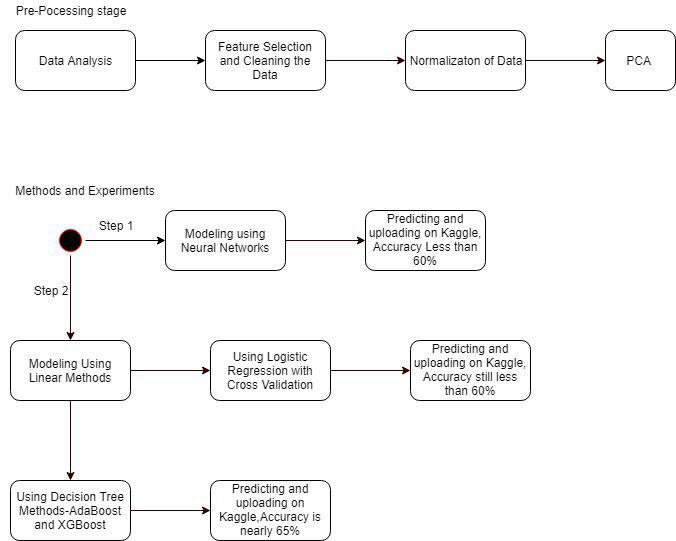
\includegraphics{img/block.jpg}

    \hypertarget{loading-of-the-csv-files-into-dataframes}{%
\subsubsection{Loading of the CSV files into
Dataframes}\label{loading-of-the-csv-files-into-dataframes}}

    \begin{Verbatim}[commandchars=\\\{\}]
{\color{incolor}In [{\color{incolor}56}]:} \PY{c+c1}{\PYZsh{} loading training data and labels into dataframes}
         \PY{n}{df\PYZus{}data} \PY{o}{=} \PY{n}{pd}\PY{o}{.}\PY{n}{read\PYZus{}csv}\PY{p}{(}\PY{l+s+s2}{\PYZdq{}}\PY{l+s+s2}{train\PYZus{}data.csv}\PY{l+s+s2}{\PYZdq{}}\PY{p}{,}\PY{n}{header}\PY{o}{=}\PY{k+kc}{None}\PY{p}{)}
         \PY{n}{df\PYZus{}labels} \PY{o}{=} \PY{n}{pd}\PY{o}{.}\PY{n}{read\PYZus{}csv}\PY{p}{(}\PY{l+s+s2}{\PYZdq{}}\PY{l+s+s2}{train\PYZus{}labels.csv}\PY{l+s+s2}{\PYZdq{}}\PY{p}{,}\PY{n}{header}\PY{o}{=}\PY{k+kc}{None}\PY{p}{,}\PY{n}{names}\PY{o}{=}\PY{p}{[}\PY{l+s+s2}{\PYZdq{}}\PY{l+s+s2}{label}\PY{l+s+s2}{\PYZdq{}}\PY{p}{]}\PY{p}{)}
         
         \PY{c+c1}{\PYZsh{} Converting the dataframes to numpy arrays to utilize in the rest of the code }
         \PY{n}{X} \PY{o}{=} \PY{n}{df\PYZus{}data}\PY{o}{.}\PY{n}{values}
         \PY{n}{y} \PY{o}{=} \PY{n}{df\PYZus{}labels}\PY{o}{.}\PY{n}{label}\PY{o}{.}\PY{n}{values}
\end{Verbatim}


    \hypertarget{preprocessing-the-data}{%
\subsection{Preprocessing the data}\label{preprocessing-the-data}}

The general method in which we pre-process the data is as follows: -
\textbf{Cleaning of the features}: We remove the MFCC columns that we
found to be corrupted in data analysis. This step may or may not be done
depending upon the model that is being used - \textbf{Normalization of
Data}: Getting all features scaled to same range is very important to
make sure that the models learn correct representations -
\textbf{Principal Component Analysis}: PCA helps reduce the overall
dimensionality of the data and also keeps the most important features in
focus

    \begin{Verbatim}[commandchars=\\\{\}]
{\color{incolor}In [{\color{incolor}17}]:} \PY{c+c1}{\PYZsh{} Import preprocessing for feature normalization}
         \PY{k+kn}{from} \PY{n+nn}{sklearn} \PY{k}{import} \PY{n}{preprocessing}
         \PY{c+c1}{\PYZsh{} Import Cross VAlidation Score}
         \PY{k+kn}{from} \PY{n+nn}{sklearn}\PY{n+nn}{.}\PY{n+nn}{model\PYZus{}selection} \PY{k}{import} \PY{n}{cross\PYZus{}val\PYZus{}score}
         \PY{c+c1}{\PYZsh{} Import Classification report and cnfusion matrix for testing }
         \PY{k+kn}{from} \PY{n+nn}{sklearn}\PY{n+nn}{.}\PY{n+nn}{metrics} \PY{k}{import} \PY{n}{classification\PYZus{}report}\PY{p}{,} \PY{n}{confusion\PYZus{}matrix}  
         \PY{c+c1}{\PYZsh{} Weak classifier for Adaboost}
         \PY{k+kn}{from} \PY{n+nn}{sklearn}\PY{n+nn}{.}\PY{n+nn}{tree} \PY{k}{import} \PY{n}{DecisionTreeClassifier}
         \PY{c+c1}{\PYZsh{} Importing seaborn for confusion matrix heatmaps }
         \PY{k+kn}{import} \PY{n+nn}{seaborn} \PY{k}{as} \PY{n+nn}{sns}
         \PY{c+c1}{\PYZsh{} testing and validation data splitting}
         \PY{k+kn}{from} \PY{n+nn}{sklearn}\PY{n+nn}{.}\PY{n+nn}{model\PYZus{}selection} \PY{k}{import} \PY{n}{train\PYZus{}test\PYZus{}split}
         \PY{c+c1}{\PYZsh{} Imbalance handling though SMOTE}
         \PY{k+kn}{from} \PY{n+nn}{imblearn}\PY{n+nn}{.}\PY{n+nn}{combine} \PY{k}{import} \PY{n}{SMOTEENN}
         \PY{c+c1}{\PYZsh{} Metrics to evaluate the model}
         \PY{k+kn}{from} \PY{n+nn}{sklearn}\PY{n+nn}{.}\PY{n+nn}{metrics} \PY{k}{import} \PY{n}{accuracy\PYZus{}score}\PY{p}{,}\PY{n}{log\PYZus{}loss}
         \PY{c+c1}{\PYZsh{} Tensorflow, Keras for NN}
         \PY{k+kn}{import} \PY{n+nn}{tensorflow} \PY{k}{as} \PY{n+nn}{tf}
         \PY{k+kn}{from} \PY{n+nn}{tensorflow} \PY{k}{import} \PY{n}{keras}
         
         \PY{c+c1}{\PYZsh{} XGBoost for gradient boosting }
         \PY{k+kn}{import} \PY{n+nn}{xgboost} \PY{k}{as} \PY{n+nn}{xgb}
         \PY{c+c1}{\PYZsh{} Logistic regression models}
         \PY{k+kn}{from} \PY{n+nn}{sklearn}\PY{n+nn}{.}\PY{n+nn}{linear\PYZus{}model} \PY{k}{import} \PY{n}{LogisticRegressionCV}\PY{p}{,}\PY{n}{LogisticRegression}
         \PY{c+c1}{\PYZsh{} Adaboost models}
         \PY{k+kn}{from} \PY{n+nn}{sklearn}\PY{n+nn}{.}\PY{n+nn}{ensemble} \PY{k}{import} \PY{n}{AdaBoostClassifier}
         \PY{c+c1}{\PYZsh{} Support vector classifier model}
         \PY{k+kn}{from} \PY{n+nn}{sklearn}\PY{n+nn}{.}\PY{n+nn}{svm} \PY{k}{import} \PY{n}{SVC}  
\end{Verbatim}


    \hypertarget{cleaning-the-data}{%
\subsection{Cleaning the Data}\label{cleaning-the-data}}

In this step we declare a function that will remove the first 4 MFCC
coefficients and all its respective statistics. This will in total
remove 16 features from all the data points and return the resultant
cleaned data

    \begin{Verbatim}[commandchars=\\\{\}]
{\color{incolor}In [{\color{incolor}18}]:} \PY{k}{def} \PY{n+nf}{clean\PYZus{}data}\PY{p}{(}\PY{n}{X}\PY{p}{)}\PY{p}{:}
             \PY{l+s+sd}{\PYZsq{}\PYZsq{}\PYZsq{}}
         \PY{l+s+sd}{    Function to clean the features by removing the first 4 MFCC columns and all their statistics}
         \PY{l+s+sd}{    \PYZsq{}\PYZsq{}\PYZsq{}}
             
             \PY{c+c1}{\PYZsh{}The first 4 columns of MFCC}
             \PY{n}{remove} \PY{o}{=} \PY{n}{np}\PY{o}{.}\PY{n}{array}\PY{p}{(}\PY{p}{[}\PY{l+m+mi}{0}\PY{p}{,}\PY{l+m+mi}{1}\PY{p}{,}\PY{l+m+mi}{2}\PY{p}{,}\PY{l+m+mi}{3}\PY{p}{]}\PY{p}{)}
             \PY{n}{remove} \PY{o}{=} \PY{n}{np}\PY{o}{.}\PY{n}{array}\PY{p}{(}\PY{p}{[}\PY{n}{remove}\PY{o}{+}\PY{n}{i}\PY{o}{*}\PY{l+m+mi}{12} \PY{k}{for} \PY{n}{i} \PY{o+ow}{in} \PY{n+nb}{range}\PY{p}{(}\PY{l+m+mi}{4}\PY{p}{)}\PY{p}{]}\PY{p}{)}
             \PY{n}{remove} \PY{o}{=} \PY{n}{remove}\PY{o}{.}\PY{n}{flatten}\PY{p}{(}\PY{p}{)}
             
             \PY{n}{remove} \PY{o}{=} \PY{n}{np}\PY{o}{.}\PY{n}{array}\PY{p}{(}\PY{n}{mfcc}\PY{p}{)}\PY{p}{[}\PY{n}{remove}\PY{p}{]}
             \PY{c+c1}{\PYZsh{} Remove the elements from the numpy array and return the clean data}
             \PY{n}{clean\PYZus{}data} \PY{o}{=} \PY{n}{np}\PY{o}{.}\PY{n}{delete}\PY{p}{(}\PY{n}{X}\PY{p}{,}\PY{n}{remove}\PY{p}{,}\PY{n}{axis}\PY{o}{=}\PY{l+m+mi}{1}\PY{p}{)}
             \PY{k}{return} \PY{n}{clean\PYZus{}data}
\end{Verbatim}


    \hypertarget{normalization-of-the-data}{%
\subsection{Normalization of the data}\label{normalization-of-the-data}}

The normalization or feature scaling is an important step for PCA as
well as machine learning. PCA will project the features into a space
with maximal variation, hence if features aren't normalized then the
components that PCA return will be incorrect. Hence before calculating
the compression matrix for the data we normalize it first. For machine
learning models like Linear Regression and Support vector Machines
(SVMs) which utilize variants of gradient descent feature scaling helps
the models converge faster when compared to models that are given
features as is.

We utilize the Sklearn's MinMaxScaler() to normalize the features.

    \begin{Verbatim}[commandchars=\\\{\}]
{\color{incolor}In [{\color{incolor}19}]:} \PY{k}{def} \PY{n+nf}{normalize}\PY{p}{(}\PY{n}{X}\PY{p}{)}\PY{p}{:}
             \PY{l+s+sd}{\PYZsq{}\PYZsq{}\PYZsq{}}
         \PY{l+s+sd}{    Function to perform feature scaling on the data using Min Max Scaling}
         \PY{l+s+sd}{    \PYZsq{}\PYZsq{}\PYZsq{}}
             
             \PY{c+c1}{\PYZsh{} Utilize the MinMaxscaler for normalization }
             \PY{n}{min\PYZus{}max\PYZus{}scaler} \PY{o}{=} \PY{n}{preprocessing}\PY{o}{.}\PY{n}{MinMaxScaler}\PY{p}{(}\PY{p}{)}
             \PY{c+c1}{\PYZsh{} Return the scaled data}
             \PY{n}{x\PYZus{}scaled} \PY{o}{=} \PY{n}{min\PYZus{}max\PYZus{}scaler}\PY{o}{.}\PY{n}{fit\PYZus{}transform}\PY{p}{(}\PY{n}{X}\PY{p}{)}
             \PY{k}{return} \PY{n}{x\PYZus{}scaled}
\end{Verbatim}


    \hypertarget{principal-component-analysis-of-features}{%
\subsection{Principal Component Analysis of
Features}\label{principal-component-analysis-of-features}}

PCA allows us to optimally compress the information contained in
high-dimensional raw feature vectors into a small set of new features,
which are called principal components (PC). {[}4{]} These new features
are then used for classification tasks. Using the PCs as features
(instead of the raw feature vectors) is beneficial in terms of
computational complexity and statistical properties.

    \begin{Verbatim}[commandchars=\\\{\}]
{\color{incolor}In [{\color{incolor}20}]:} \PY{k}{def} \PY{n+nf}{compute\PYZus{}pca}\PY{p}{(}\PY{n}{Z}\PY{p}{,} \PY{n}{d}\PY{p}{)}\PY{p}{:}
             \PY{l+s+sd}{\PYZsq{}\PYZsq{}\PYZsq{}}
         \PY{l+s+sd}{    Input: the N by D data matrix Z, the number of components d}
         \PY{l+s+sd}{    Output: a d by D matrix W\PYZus{}pca, and all eigenvalues of Q}
         \PY{l+s+sd}{    \PYZsq{}\PYZsq{}\PYZsq{}}
             \PY{n}{N} \PY{o}{=} \PY{n}{Z}\PY{o}{.}\PY{n}{shape}\PY{p}{[}\PY{l+m+mi}{0}\PY{p}{]}
             \PY{n}{Q} \PY{o}{=} \PY{l+m+mi}{1}\PY{o}{/}\PY{n}{N}\PY{o}{*}\PY{p}{(}\PY{n}{Z}\PY{o}{.}\PY{n}{T}\PY{n+nd}{@Z}\PY{p}{)}
         
             \PY{n}{values}\PY{p}{,}\PY{n}{vectors} \PY{o}{=} \PY{n}{np}\PY{o}{.}\PY{n}{linalg}\PY{o}{.}\PY{n}{eig}\PY{p}{(}\PY{n}{Q}\PY{p}{)}
         
             \PY{n}{sort}  \PY{o}{=} \PY{n}{np}\PY{o}{.}\PY{n}{argsort}\PY{p}{(}\PY{n}{values}\PY{p}{)}
             \PY{n}{largest} \PY{o}{=} \PY{n}{sort}\PY{p}{[}\PY{o}{\PYZhy{}}\PY{n}{d}\PY{p}{:}\PY{p}{]}\PY{p}{[}\PY{p}{:}\PY{p}{:}\PY{o}{\PYZhy{}}\PY{l+m+mi}{1}\PY{p}{]}
             \PY{n}{W\PYZus{}pca} \PY{o}{=} \PY{n}{vectors}\PY{p}{[}\PY{p}{:}\PY{p}{,}\PY{n}{largest}\PY{p}{]}
             \PY{n}{W\PYZus{}pca} \PY{o}{=} \PY{n}{W\PYZus{}pca}\PY{o}{.}\PY{n}{T}
             \PY{n}{eigvalues} \PY{o}{=} \PY{n}{values}
             
             \PY{k}{return} \PY{n}{W\PYZus{}pca}\PY{o}{.}\PY{n}{real}\PY{p}{,}\PY{n}{eigvalues}
         
         \PY{k}{def} \PY{n+nf}{compression}\PY{p}{(}\PY{n}{X}\PY{p}{,}\PY{n}{PCA}\PY{p}{,}\PY{n}{num\PYZus{}dims}\PY{p}{)}\PY{p}{:}
             \PY{l+s+sd}{\PYZsq{}\PYZsq{}\PYZsq{}}
         \PY{l+s+sd}{    A function that compresses the data X into num\PYZus{}dims dimensions using the PCA matrix}
         \PY{l+s+sd}{    \PYZsq{}\PYZsq{}\PYZsq{}}
             
             \PY{n}{compr} \PY{o}{=} \PY{n}{X} \PY{o}{@} \PY{n}{PCA}\PY{p}{[}\PY{p}{:}\PY{n}{num\PYZus{}dims}\PY{p}{,}\PY{p}{:}\PY{p}{]}\PY{o}{.}\PY{n}{T}
             \PY{k}{return} \PY{n}{compr}
\end{Verbatim}


    \begin{Verbatim}[commandchars=\\\{\}]
{\color{incolor}In [{\color{incolor}21}]:} \PY{k}{def} \PY{n+nf}{plot\PYZus{}error}\PY{p}{(}\PY{n}{eigvalues}\PY{p}{,}\PY{n}{max\PYZus{}d}\PY{p}{)}\PY{p}{:}
             \PY{l+s+sd}{\PYZsq{}\PYZsq{}\PYZsq{}}
         \PY{l+s+sd}{    Function to visualize the reconstruction error of PCA f}
         \PY{l+s+sd}{    \PYZsq{}\PYZsq{}\PYZsq{}}
             
             \PY{n}{x}\PY{o}{=}\PY{n+nb}{range}\PY{p}{(}\PY{l+m+mi}{1}\PY{p}{,}\PY{n}{max\PYZus{}d}\PY{o}{+}\PY{l+m+mi}{1}\PY{p}{)}
             \PY{n}{errors}\PY{o}{=}\PY{p}{[}\PY{n+nb}{sum}\PY{p}{(}\PY{n}{eigvalues}\PY{p}{[}\PY{n}{d}\PY{p}{:}\PY{p}{]}\PY{p}{)} \PY{k}{for} \PY{n}{d} \PY{o+ow}{in} \PY{n}{x}\PY{p}{]}
             \PY{n}{plt}\PY{o}{.}\PY{n}{plot}\PY{p}{(}\PY{n}{x}\PY{p}{,}\PY{n}{errors}\PY{p}{)}
             \PY{n}{plt}\PY{o}{.}\PY{n}{xlabel}\PY{p}{(}\PY{l+s+s1}{\PYZsq{}}\PY{l+s+s1}{Number of principal components \PYZdl{}d\PYZdl{}}\PY{l+s+s1}{\PYZsq{}}\PY{p}{)}
             \PY{n}{plt}\PY{o}{.}\PY{n}{ylabel}\PY{p}{(}\PY{l+s+s1}{\PYZsq{}}\PY{l+s+s1}{Reconstruction error \PYZdl{}}\PY{l+s+s1}{\PYZbs{}}\PY{l+s+s1}{mathcal}\PY{l+s+si}{\PYZob{}E\PYZcb{}}\PY{l+s+s1}{\PYZdl{}}\PY{l+s+s1}{\PYZsq{}}\PY{p}{)}
             \PY{n}{plt}\PY{o}{.}\PY{n}{title}\PY{p}{(}\PY{l+s+s1}{\PYZsq{}}\PY{l+s+s1}{Number of principal components vs the reconstruction error}\PY{l+s+s1}{\PYZsq{}}\PY{p}{)}
             \PY{n}{plt}\PY{o}{.}\PY{n}{show}\PY{p}{(}\PY{p}{)}
\end{Verbatim}


    \hypertarget{reconstruction-error-of-pca}{%
\subsubsection{Reconstruction Error of
PCA}\label{reconstruction-error-of-pca}}

To see how many principal components we need to select to ensure that
the error is minimal we plot a reconstruction error graph. From the
graph we see that beyond 150 principal components the error is minimal
and the reduction in features size is considerable.

    \begin{Verbatim}[commandchars=\\\{\}]
{\color{incolor}In [{\color{incolor}22}]:} \PY{n}{mpl}\PY{o}{.}\PY{n}{rcParams}\PY{p}{[}\PY{l+s+s1}{\PYZsq{}}\PY{l+s+s1}{figure.dpi}\PY{l+s+s1}{\PYZsq{}}\PY{p}{]}\PY{o}{=}\PY{l+m+mi}{130}
         \PY{c+c1}{\PYZsh{} Compute the PCA matrix}
         \PY{n}{PCA}\PY{p}{,}\PY{n}{eigvals} \PY{o}{=} \PY{n}{compute\PYZus{}pca}\PY{p}{(}\PY{n}{Z}\PY{o}{=}\PY{n}{normalize}\PY{p}{(}\PY{n}{X}\PY{p}{)}\PY{p}{,}\PY{n}{d}\PY{o}{=}\PY{l+m+mi}{264}\PY{p}{)}
         \PY{c+c1}{\PYZsh{} Visualize the PCA reconstruction errors}
         \PY{n}{plot\PYZus{}error}\PY{p}{(}\PY{n}{eigvals}\PY{p}{,}\PY{l+m+mi}{264}\PY{p}{)}
\end{Verbatim}


    \begin{center}
    \adjustimage{max size={0.9\linewidth}{0.9\paperheight}}{output_43_0.png}
    \end{center}
    { \hspace*{\fill} \\}
    
    \hypertarget{methods-for-hyper-parameter-tuning}{%
\subsection{Methods for Hyper Parameter
Tuning}\label{methods-for-hyper-parameter-tuning}}

Many of the models that is considered in the project have various
parameters that can be tunes to increase the performance and accuracy of
the trained model. Some of the hyper parameters and explanation of the
values that can be used for some of the models used in the project are
as follows: 1. Neural Networks: - Optimizer : RMSProp,Adam, AdaGrad etc
- Layers : Number of hidden layers - Neurons : Number of neurons in each
layer - Activation : Sigmoid, ReLu, SeLu - Dropout : Fraction of inputs
to be dropped, combats overfitting 2. Linear Regression: - Optimizer :
Newton-cg, LBFGS, SAGA - C : Inverse of L2 regularization parameter 3.
XGBoost : - Depth : maximum tree depth for the weak estimators - eta :
step shrinkage size, combats overfitting - Lambda : L2 regularization
parameter - metric : evaluation metric for validation

    \hypertarget{cross-validation}{%
\subsection{Cross Validation}\label{cross-validation}}

The easiest way to to tune for hyper parameters is through cross
validation. Cross validation is when the dataset is split into 3
portions: 1. Training 2. Cross Validation 3. Testing

This method will train the model on the testing data and evaluate is
performance on the Cross Validation data. The model whose parameter
yields the best cross validation score will be one that will used to
predict from the test dataset. Through this process we can can
parameters that will make the model perform better on test data. The
only drawback with this method is that with limited data, the splits
result in very small number of samples in each set. Models such as
neural networks do not work well with lesser data points hence will
perform poorly.

\hypertarget{k-folds}{%
\subsubsection{K Folds}\label{k-folds}}

A method that can work even when the size of the data is small is
KFolds. Assume that we are doing 4 folds cross validation, then we
divide the data into \(k\) parts and during every \(k^th\) iteration we
leave out the \(k^th\) portion of the data as testing data and use the
remaining as training data. Then after performing \(k\) iterations we
can calculate the average of the metric that we have chosen to get the
cross-validation score. This cross validation score allows us to compare
models with different hyper-parameters and choose the one with the est
cross-validation score. The best benefit of Kfolds is that it is not
affected by classes or groups, hence will perform well with our
imbalance in the data A simple diagram explaining the Kfolds cross
validation for \(k=4\): 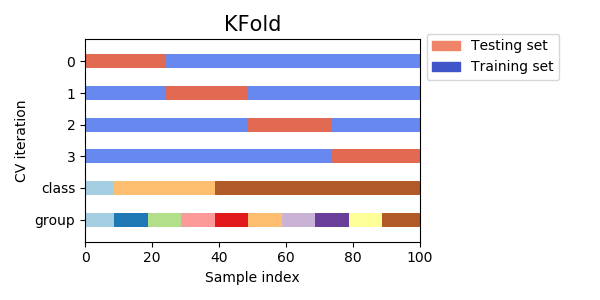
\includegraphics{img/kfolds.png}

    \begin{Verbatim}[commandchars=\\\{\}]
{\color{incolor}In [{\color{incolor}23}]:} \PY{k}{def} \PY{n+nf}{get\PYZus{}splits}\PY{p}{(}\PY{n}{X}\PY{p}{,}\PY{n}{labels}\PY{p}{,}\PY{n}{test\PYZus{}size}\PY{o}{=}\PY{l+m+mf}{0.4}\PY{p}{,}\PY{n}{val\PYZus{}size}\PY{o}{=}\PY{l+m+mf}{0.4}\PY{p}{,}\PY{n}{random\PYZus{}state}\PY{o}{=}\PY{l+m+mi}{0}\PY{p}{,}\PY{n}{smote}\PY{o}{=}\PY{k+kc}{False}\PY{p}{,}\PY{n}{validation}\PY{o}{=}\PY{k+kc}{True}\PY{p}{)}\PY{p}{:}
             \PY{l+s+sd}{\PYZsq{}\PYZsq{}\PYZsq{}}
         \PY{l+s+sd}{    Function to get the training and tesing splits}
         \PY{l+s+sd}{    }
         \PY{l+s+sd}{    smote     : Boolean option to specify whether or not to perform SMOTE on the training data split}
         \PY{l+s+sd}{    validation : Boolean option to specify if a validation split is needed or not}
         \PY{l+s+sd}{    \PYZsq{}\PYZsq{}\PYZsq{}}
             \PY{c+c1}{\PYZsh{} Perform a Train Test split irrespective of options}
             \PY{n}{X\PYZus{}train}\PY{p}{,}\PY{n}{X\PYZus{}test}\PY{p}{,}\PY{n}{y\PYZus{}train}\PY{p}{,}\PY{n}{y\PYZus{}test}\PY{o}{=} \PY{n}{train\PYZus{}test\PYZus{}split}\PY{p}{(}\PY{n}{X}\PY{p}{,}\PY{n}{y}\PY{p}{,} \PY{n}{test\PYZus{}size}\PY{o}{=}\PY{n}{test\PYZus{}size}\PY{p}{,} \PY{n}{random\PYZus{}state}\PY{o}{=}\PY{n}{random\PYZus{}state}\PY{p}{)}
             
             \PY{c+c1}{\PYZsh{} If validation is needed split the train further into train and validation}
             \PY{k}{if} \PY{n}{validation} \PY{o}{==} \PY{k+kc}{True}\PY{p}{:}
                 
                 \PY{n}{X\PYZus{}train}\PY{p}{,}\PY{n}{X\PYZus{}val}\PY{p}{,}\PY{n}{y\PYZus{}train}\PY{p}{,}\PY{n}{y\PYZus{}val}\PY{o}{=} \PY{n}{train\PYZus{}test\PYZus{}split}\PY{p}{(}\PY{n}{X\PYZus{}train}\PY{p}{,}\PY{n}{y\PYZus{}train}\PY{p}{,} \PY{n}{test\PYZus{}size}\PY{o}{=}\PY{n}{val\PYZus{}size}\PY{p}{,} \PY{n}{random\PYZus{}state}\PY{o}{=}\PY{n}{random\PYZus{}state}\PY{p}{)}
         
                 \PY{k}{if} \PY{n}{smote} \PY{o}{==}\PY{k+kc}{False}\PY{p}{:}
                     \PY{k}{return} \PY{n}{X\PYZus{}train}\PY{p}{,}\PY{n}{X\PYZus{}val}\PY{p}{,}\PY{n}{X\PYZus{}test}\PY{p}{,}\PY{n}{y\PYZus{}train}\PY{p}{,}\PY{n}{y\PYZus{}val}\PY{p}{,}\PY{n}{y\PYZus{}test}
                 \PY{n}{sm} \PY{o}{=} \PY{n}{SMOTEENN}\PY{p}{(}\PY{n}{random\PYZus{}state}\PY{o}{=}\PY{n}{random\PYZus{}state}\PY{p}{)}
         
                 \PY{n}{X\PYZus{}res}\PY{p}{,} \PY{n}{y\PYZus{}res} \PY{o}{=} \PY{n}{sm}\PY{o}{.}\PY{n}{fit\PYZus{}resample}\PY{p}{(}\PY{n}{X\PYZus{}train}\PY{p}{,} \PY{n}{y\PYZus{}train}\PY{p}{)}
                 \PY{k}{return} \PY{n}{X\PYZus{}res}\PY{p}{,}\PY{n}{X\PYZus{}val}\PY{p}{,}\PY{n}{X\PYZus{}test}\PY{p}{,}\PY{n}{y\PYZus{}res}\PY{p}{,}\PY{n}{y\PYZus{}val}\PY{p}{,}\PY{n}{y\PYZus{}test}
             
             \PY{k}{else}\PY{p}{:}
                 \PY{k}{if} \PY{n}{smote} \PY{o}{==}\PY{k+kc}{False}\PY{p}{:}
                     \PY{k}{return} \PY{n}{X\PYZus{}train}\PY{p}{,}\PY{n}{X\PYZus{}test}\PY{p}{,}\PY{n}{y\PYZus{}train}\PY{p}{,}\PY{n}{y\PYZus{}test}
                 \PY{n}{sm} \PY{o}{=} \PY{n}{SMOTEENN}\PY{p}{(}\PY{n}{random\PYZus{}state}\PY{o}{=}\PY{n}{random\PYZus{}state}\PY{p}{)}
         
                 \PY{n}{X\PYZus{}res}\PY{p}{,} \PY{n}{y\PYZus{}res} \PY{o}{=} \PY{n}{sm}\PY{o}{.}\PY{n}{fit\PYZus{}resample}\PY{p}{(}\PY{n}{X\PYZus{}train}\PY{p}{,} \PY{n}{y\PYZus{}train}\PY{p}{)}
                 \PY{k}{return} \PY{n}{X\PYZus{}res}\PY{p}{,}\PY{n}{X\PYZus{}test}\PY{p}{,}\PY{n}{y\PYZus{}res}\PY{p}{,}\PY{n}{y\PYZus{}test}
\end{Verbatim}


    \hypertarget{oversampling-to-handle-imbalance}{%
\subsection{Oversampling to Handle
Imbalance}\label{oversampling-to-handle-imbalance}}

There are 2 broad methods to handle imbalances in a database: 1.
Under-Sampling: In this method we take fewer examples from classes that
have larger representation so that we balance the number of examples
from the class that is in the minority. This method does not introduce
any noise in the training data but may reduce the total number of
samples that can be trained on by a significant amount. Hence
under-sampling is used when the even the minority class has a
sufficiently large number of samples. 2. Over-Sampling: In over-sampling
we create synthetic data for the classes that are in the minority. The
creation of these extra samples is through a perturbation and hence can
increase significant noise in very high dimensional datasets.

Given the already small dataset at our disposal, the method that we
chose to explore is over-sampling and in specific Synthetic Minority
Over-Sampling Technique (SMOTE) {[}5{]}

\hypertarget{smote}{%
\subsubsection{SMOTE}\label{smote}}

This method creates synthetic samples for a data point in the minority
class by taking samples of the feature space for each target class and
its nearest neighbors, and generates new examples that combine features
of the target case with features of its neighbors. This approach
increases the features available to each class and makes the samples
more general. As mentioned in the original paper {[}5{]} there are more
advanced sampling that combine both oversampling of minority classes and
under-sampling majority classes to achieve better results in metrics
such as Area under ROC curve (AOC) and F1-score.

The issue is the in data with many features the feature space is so
large for classes that addition of even slightly perturbed samples will
cause major changes in decision boundaries in the dataset. In this
project we will utilize \textbf{imblearn} package to implement SMOTE to
try and handle the imbalances in the database.

    \hypertarget{report-of-the-test-evaluation}{%
\subsection{Report of the Test
Evaluation}\label{report-of-the-test-evaluation}}

To evaluate the performance of any model we need to compare test
results. The metrics that we monitor are the \textbf{accuracy score} and
\textbf{multi-class log loss} of the model. In most cross-validation
trials also we be using the same metrics.

One thing to note is that in datasets with imbalances the accuracy is
not a good measure of the quality of the classifier. So we also monitor
the \textbf{precison},\textbf{recall} and \textbf{f1-score} of the model
(sometimes the \textbf{aoc(area under ROC curve)} ) after predicting on
the test set. But as these metrics are not the one that will not be
displayed in the report as there is already information of the
performance from the \textbf{confusion matrix} and the accuracy scores.

    \begin{Verbatim}[commandchars=\\\{\}]
{\color{incolor}In [{\color{incolor}25}]:} \PY{k}{def} \PY{n+nf}{report}\PY{p}{(}\PY{n}{y\PYZus{}pred}\PY{p}{,}\PY{n}{y\PYZus{}test}\PY{p}{,}\PY{n}{y\PYZus{}prob}\PY{p}{)}\PY{p}{:}
             \PY{l+s+sd}{\PYZsq{}\PYZsq{}\PYZsq{}}
         \PY{l+s+sd}{    Function that prints a report of the test evalutaion. }
         \PY{l+s+sd}{    It outputs a confusion matrix and the accuracy score and logloss of the model}
         \PY{l+s+sd}{    \PYZsq{}\PYZsq{}\PYZsq{}}
             
             \PY{n}{mpl}\PY{o}{.}\PY{n}{rcParams}\PY{p}{[}\PY{l+s+s1}{\PYZsq{}}\PY{l+s+s1}{figure.dpi}\PY{l+s+s1}{\PYZsq{}}\PY{p}{]}\PY{o}{=}\PY{l+m+mi}{80}
             \PY{c+c1}{\PYZsh{} Calculate the log loss }
             \PY{n}{logloss} \PY{o}{=} \PY{n}{log\PYZus{}loss}\PY{p}{(}\PY{n}{y\PYZus{}test}\PY{p}{,} \PY{n}{y\PYZus{}prob}\PY{p}{)}
             
             \PY{c+c1}{\PYZsh{} Confusion matrix}
             \PY{n}{cm} \PY{o}{=} \PY{n}{confusion\PYZus{}matrix}\PY{p}{(}\PY{n}{y\PYZus{}test}\PY{p}{,} \PY{n}{y\PYZus{}pred}\PY{p}{)}
            
             \PY{n}{cm} \PY{o}{=} \PY{n}{cm} \PY{o}{/} \PY{n}{cm}\PY{o}{.}\PY{n}{astype}\PY{p}{(}\PY{n}{np}\PY{o}{.}\PY{n}{float}\PY{p}{)}\PY{o}{.}\PY{n}{sum}\PY{p}{(}\PY{n}{axis}\PY{o}{=}\PY{l+m+mi}{1}\PY{p}{)}
             
             \PY{c+c1}{\PYZsh{} Calculate the score}
             \PY{n}{score} \PY{o}{=} \PY{n}{accuracy\PYZus{}score}\PY{p}{(}\PY{n}{y\PYZus{}test}\PY{p}{,}\PY{n}{y\PYZus{}pred}\PY{p}{)}
             
             \PY{n}{mpl}\PY{o}{.}\PY{n}{rcParams}\PY{p}{[}\PY{l+s+s1}{\PYZsq{}}\PY{l+s+s1}{figure.dpi}\PY{l+s+s1}{\PYZsq{}}\PY{p}{]}\PY{o}{=}\PY{l+m+mi}{80}
             
             \PY{n}{df} \PY{o}{=} \PY{n}{pd}\PY{o}{.}\PY{n}{DataFrame}\PY{p}{(}\PY{n}{cm}\PY{p}{,}\PY{n}{index}\PY{o}{=}\PY{n}{classes}\PY{p}{,}\PY{n}{columns}\PY{o}{=}\PY{n}{classes}\PY{p}{)}
             \PY{n}{plt}\PY{o}{.}\PY{n}{figure}\PY{p}{(}\PY{n}{figsize}\PY{o}{=}\PY{p}{(}\PY{l+m+mi}{9}\PY{p}{,}\PY{l+m+mi}{9}\PY{p}{)}\PY{p}{)}
             \PY{n}{heatmap} \PY{o}{=} \PY{n}{sns}\PY{o}{.}\PY{n}{heatmap}\PY{p}{(}\PY{n}{df}\PY{p}{,} \PY{n}{annot}\PY{o}{=}\PY{k+kc}{True}\PY{p}{,} \PY{n}{fmt}\PY{o}{=}\PY{l+s+s2}{\PYZdq{}}\PY{l+s+s2}{.3f}\PY{l+s+s2}{\PYZdq{}}\PY{p}{,} \PY{n}{linewidths}\PY{o}{=}\PY{o}{.}\PY{l+m+mi}{5}\PY{p}{,} \PY{n}{square} \PY{o}{=} \PY{k+kc}{True}\PY{p}{,} \PY{n}{cmap} \PY{o}{=} \PY{l+s+s1}{\PYZsq{}}\PY{l+s+s1}{Blues}\PY{l+s+s1}{\PYZsq{}}\PY{p}{)}\PY{p}{;}
             \PY{n}{heatmap}\PY{o}{.}\PY{n}{yaxis}\PY{o}{.}\PY{n}{set\PYZus{}ticklabels}\PY{p}{(}\PY{n}{heatmap}\PY{o}{.}\PY{n}{yaxis}\PY{o}{.}\PY{n}{get\PYZus{}ticklabels}\PY{p}{(}\PY{p}{)}\PY{p}{,} \PY{n}{rotation}\PY{o}{=}\PY{l+m+mi}{0}\PY{p}{,} \PY{n}{ha}\PY{o}{=}\PY{l+s+s1}{\PYZsq{}}\PY{l+s+s1}{right}\PY{l+s+s1}{\PYZsq{}}\PY{p}{)}
             \PY{n}{heatmap}\PY{o}{.}\PY{n}{xaxis}\PY{o}{.}\PY{n}{set\PYZus{}ticklabels}\PY{p}{(}\PY{n}{heatmap}\PY{o}{.}\PY{n}{xaxis}\PY{o}{.}\PY{n}{get\PYZus{}ticklabels}\PY{p}{(}\PY{p}{)}\PY{p}{,} \PY{n}{rotation}\PY{o}{=}\PY{l+m+mi}{45}\PY{p}{,} \PY{n}{ha}\PY{o}{=}\PY{l+s+s1}{\PYZsq{}}\PY{l+s+s1}{right}\PY{l+s+s1}{\PYZsq{}}\PY{p}{)}
             \PY{n}{plt}\PY{o}{.}\PY{n}{ylabel}\PY{p}{(}\PY{l+s+s1}{\PYZsq{}}\PY{l+s+s1}{Actual label}\PY{l+s+s1}{\PYZsq{}}\PY{p}{)}\PY{p}{;}
             \PY{n}{plt}\PY{o}{.}\PY{n}{xlabel}\PY{p}{(}\PY{l+s+s1}{\PYZsq{}}\PY{l+s+s1}{Predicted label}\PY{l+s+s1}{\PYZsq{}}\PY{p}{)}
             \PY{n}{all\PYZus{}sample\PYZus{}title} \PY{o}{=} \PY{l+s+s1}{\PYZsq{}}\PY{l+s+s1}{Accuracy :}\PY{l+s+si}{\PYZob{}0:.4f\PYZcb{}}\PY{l+s+s1}{ }\PY{l+s+se}{\PYZbs{}n}\PY{l+s+s1}{Logloss: }\PY{l+s+si}{\PYZob{}1:.4f\PYZcb{}}\PY{l+s+s1}{\PYZsq{}}\PY{o}{.}\PY{n}{format}\PY{p}{(}\PY{n}{score}\PY{p}{,}\PY{n}{logloss}\PY{p}{)}
             \PY{n}{plt}\PY{o}{.}\PY{n}{title}\PY{p}{(}\PY{n}{all\PYZus{}sample\PYZus{}title}\PY{p}{,} \PY{n}{size} \PY{o}{=} \PY{l+m+mi}{15}\PY{p}{)}
             \PY{c+c1}{\PYZsh{} Print the F1 score classification report}
             \PY{c+c1}{\PYZsh{}classification\PYZus{}report(y\PYZus{}test,y\PYZus{}pred)}
             \PY{n}{plt}\PY{o}{.}\PY{n}{show}\PY{p}{(}\PY{p}{)}
\end{Verbatim}


    \hypertarget{approaches}{%
\subsection{Approaches}\label{approaches}}

In trying to effectively classify the genres we chose to see the
efficacy of non-linear vs linear machine learning models. The models
that were experimented with are : 1. Neural Networks 2. Logistic
Regression 3. Gradient Boosting

    \hypertarget{neural-networks}{%
\subsubsection{Neural Networks}\label{neural-networks}}

A neural network is a computational model based on the structure and
functions of biological neural networks. Information that flows through
the network affects the structure of the NN because a neural network
changes - or learns, in a sense - based on that input and output.
{[}6{]} NNs are considered nonlinear statistical data modeling tools
where the complex relationships between inputs and outputs are modeled
or patterns are found.

    \hypertarget{logistic-regression}{%
\subsubsection{Logistic Regression}\label{logistic-regression}}

Logistic regression is a statistical method for analysing a dataset in
which there are one or more independent variables that determine an
outcome. The outcome is measured with a dichotomous variable (in which
there are only two possible outcomes). It is used to predict a binary
outcome (1 / 0, Yes / No, True / False) given a set of independent
variables. You can also think of logistic regression as a special case
of linear regression when the outcome variable is categorical, where we
are using log of odds as dependent variable. In simple words, it
predicts the probability of occurrence of an event by fitting data to a
logit function.

    \hypertarget{gradient-boosting}{%
\subsubsection{Gradient Boosting}\label{gradient-boosting}}

Lets first define what Boosting is,it is an ensemble technique for
creating collection of powerful predictors, and Gradient Boosting is a
technique for producing regression models consisting of collections of
regressors.

An ensemble is a collection of predictors whose predictions are combined
usually by some sort of weighted average or vote in order to provide an
overall prediction that takes its guidance from the collection itself.
So boosting is an ensemble technique in which learners are learned
sequentially with early learners fitting simple models to the data and
then analyzing the data for errors, those errors identify problems or
particular instances of the data that are difficult or hard to fit, as a
consequence later models focus primarily on those examples trying to get
them right.

At the end, all the models contribute with weights and the set is
combined into some overall predictors, so boosting is a method of
converting a sequence of weak learners into a very complex predictor,
it's a way of increasing the complexity of a particular model initial
learners tend to be very simple and then the weighted combination can
grow more and more complex as learners are added. {[}7{]}

The two main gradient boosting techniques that were explored in the
project were: 1. AdaBoost 2. XGBoost

    \hypertarget{results}{%
\section{Results}\label{results}}

Now we will discuss the results obtained from implementing the methods
that were discussed in the previous section. Each implementation will be
explained in some detail and the results analyzed superficially, the
proper discussion of the implication of the results will be discussed in
the next section

    \hypertarget{neural-networks}{%
\subsection{Neural Networks}\label{neural-networks}}

The first method that was tested was a Neural Network. There was a cross
validation done using a validation split of the dataset and tuning was
done for the number of layers and the number of neurons per layer and
the dropout fraction. {[}6{]}

First to analyze the neural network we utilize the \textbf{validation
loss} and \textbf{validation accuracy} graphs along with training loss
and accuracy.This gives us information if the NN starts to overfit the
training data.

    \begin{Verbatim}[commandchars=\\\{\}]
{\color{incolor}In [{\color{incolor}26}]:} \PY{k}{def} \PY{n+nf}{plot\PYZus{}history}\PY{p}{(}\PY{n}{history}\PY{p}{)}\PY{p}{:}
             \PY{l+s+sd}{\PYZsq{}\PYZsq{}\PYZsq{}}
         \PY{l+s+sd}{    Function that plots the Validation loss and accuracy along with trianing loss and accuracy.}
         \PY{l+s+sd}{    \PYZsq{}\PYZsq{}\PYZsq{}}
             
             \PY{n}{mpl}\PY{o}{.}\PY{n}{rcParams}\PY{p}{[}\PY{l+s+s1}{\PYZsq{}}\PY{l+s+s1}{figure.dpi}\PY{l+s+s1}{\PYZsq{}}\PY{p}{]}\PY{o}{=}\PY{l+m+mi}{80}
             \PY{n}{plt}\PY{o}{.}\PY{n}{figure}\PY{p}{(}\PY{p}{)}
             \PY{n}{plt}\PY{o}{.}\PY{n}{xlabel}\PY{p}{(}\PY{l+s+s1}{\PYZsq{}}\PY{l+s+s1}{Epoch}\PY{l+s+s1}{\PYZsq{}}\PY{p}{)}
             \PY{n}{plt}\PY{o}{.}\PY{n}{ylabel}\PY{p}{(}\PY{l+s+s1}{\PYZsq{}}\PY{l+s+s1}{Loss}\PY{l+s+s1}{\PYZsq{}}\PY{p}{)}
             \PY{n}{plt}\PY{o}{.}\PY{n}{plot}\PY{p}{(}\PY{n}{history}\PY{o}{.}\PY{n}{epoch}\PY{p}{,} \PY{n}{np}\PY{o}{.}\PY{n}{array}\PY{p}{(}\PY{n}{history}\PY{o}{.}\PY{n}{history}\PY{p}{[}\PY{l+s+s1}{\PYZsq{}}\PY{l+s+s1}{loss}\PY{l+s+s1}{\PYZsq{}}\PY{p}{]}\PY{p}{)}\PY{p}{,}
                    \PY{n}{label}\PY{o}{=}\PY{l+s+s1}{\PYZsq{}}\PY{l+s+s1}{Train Loss}\PY{l+s+s1}{\PYZsq{}}\PY{p}{)}
             \PY{n}{plt}\PY{o}{.}\PY{n}{plot}\PY{p}{(}\PY{n}{history}\PY{o}{.}\PY{n}{epoch}\PY{p}{,} \PY{n}{np}\PY{o}{.}\PY{n}{array}\PY{p}{(}\PY{n}{history}\PY{o}{.}\PY{n}{history}\PY{p}{[}\PY{l+s+s1}{\PYZsq{}}\PY{l+s+s1}{val\PYZus{}loss}\PY{l+s+s1}{\PYZsq{}}\PY{p}{]}\PY{p}{)}\PY{p}{,}
                    \PY{n}{label} \PY{o}{=} \PY{l+s+s1}{\PYZsq{}}\PY{l+s+s1}{Val loss}\PY{l+s+s1}{\PYZsq{}}\PY{p}{)}
             \PY{n}{plt}\PY{o}{.}\PY{n}{title}\PY{p}{(}\PY{l+s+s1}{\PYZsq{}}\PY{l+s+s1}{Model Training vs Validation loss}\PY{l+s+s1}{\PYZsq{}}\PY{p}{)}
             \PY{n}{plt}\PY{o}{.}\PY{n}{legend}\PY{p}{(}\PY{p}{)}
             \PY{n}{plt}\PY{o}{.}\PY{n}{show}\PY{p}{(}\PY{p}{)}
             \PY{n}{plt}\PY{o}{.}\PY{n}{figure}\PY{p}{(}\PY{p}{)}
             \PY{n}{plt}\PY{o}{.}\PY{n}{xlabel}\PY{p}{(}\PY{l+s+s1}{\PYZsq{}}\PY{l+s+s1}{Epoch}\PY{l+s+s1}{\PYZsq{}}\PY{p}{)}
             \PY{n}{plt}\PY{o}{.}\PY{n}{ylabel}\PY{p}{(}\PY{l+s+s1}{\PYZsq{}}\PY{l+s+s1}{Accuracy}\PY{l+s+s1}{\PYZsq{}}\PY{p}{)}
             \PY{n}{plt}\PY{o}{.}\PY{n}{plot}\PY{p}{(}\PY{n}{history}\PY{o}{.}\PY{n}{epoch}\PY{p}{,} \PY{n}{np}\PY{o}{.}\PY{n}{array}\PY{p}{(}\PY{n}{history}\PY{o}{.}\PY{n}{history}\PY{p}{[}\PY{l+s+s1}{\PYZsq{}}\PY{l+s+s1}{acc}\PY{l+s+s1}{\PYZsq{}}\PY{p}{]}\PY{p}{)}\PY{p}{,}
                    \PY{n}{label}\PY{o}{=}\PY{l+s+s1}{\PYZsq{}}\PY{l+s+s1}{Train Accuracy}\PY{l+s+s1}{\PYZsq{}}\PY{p}{)}
             \PY{n}{plt}\PY{o}{.}\PY{n}{plot}\PY{p}{(}\PY{n}{history}\PY{o}{.}\PY{n}{epoch}\PY{p}{,} \PY{n}{np}\PY{o}{.}\PY{n}{array}\PY{p}{(}\PY{n}{history}\PY{o}{.}\PY{n}{history}\PY{p}{[}\PY{l+s+s1}{\PYZsq{}}\PY{l+s+s1}{val\PYZus{}acc}\PY{l+s+s1}{\PYZsq{}}\PY{p}{]}\PY{p}{)}\PY{p}{,}
                    \PY{n}{label} \PY{o}{=} \PY{l+s+s1}{\PYZsq{}}\PY{l+s+s1}{Val Accuracy}\PY{l+s+s1}{\PYZsq{}}\PY{p}{)}
             \PY{n}{plt}\PY{o}{.}\PY{n}{title}\PY{p}{(}\PY{l+s+s1}{\PYZsq{}}\PY{l+s+s1}{Model Training vs Validation Accuracy}\PY{l+s+s1}{\PYZsq{}}\PY{p}{)}
             \PY{n}{plt}\PY{o}{.}\PY{n}{legend}\PY{p}{(}\PY{p}{)}
             \PY{n}{plt}\PY{o}{.}\PY{n}{show}\PY{p}{(}\PY{p}{)}
             
             
\end{Verbatim}


    \hypertarget{testing-nn}{%
\subsubsection{Testing NN}\label{testing-nn}}

The function below was designed to be used either for evaluating or
testing a specific NN implementation. It can be used with the \(cv\)
parameter to cross validate data. From the cross validation performed
the results obtained were : - 3 hidden layers perform better than 2
hidden layers - a dropout ratio of 0.2 produced optimal performance
without too much over-fitting - Adam was the best optimizer

    \begin{Verbatim}[commandchars=\\\{\}]
{\color{incolor}In [{\color{incolor}27}]:} \PY{k}{def} \PY{n+nf}{test\PYZus{}nn}\PY{p}{(}\PY{n}{X}\PY{p}{,}\PY{n}{y}\PY{p}{,}\PY{n}{num\PYZus{}epochs}\PY{o}{=}\PY{l+m+mi}{100}\PY{p}{,}\PY{n}{batch\PYZus{}size}\PY{o}{=}\PY{l+m+mi}{32}\PY{p}{,}\PY{n}{drop\PYZus{}out}\PY{o}{=}\PY{l+m+mf}{0.2}\PY{p}{,}\PY{n}{num\PYZus{}neurons}\PY{o}{=}\PY{l+m+mi}{128}\PY{p}{,}\PY{n}{cv}\PY{o}{=}\PY{k+kc}{False}\PY{p}{,}\PY{n}{smote}\PY{o}{=}\PY{k+kc}{False}\PY{p}{)}\PY{p}{:}
             \PY{l+s+sd}{\PYZsq{}\PYZsq{}\PYZsq{}}
         \PY{l+s+sd}{    Function that trains a NN and tests it against the test data set}
         \PY{l+s+sd}{    }
         \PY{l+s+sd}{    num\PYZus{}epochs  : How many epochs to train the NN for}
         \PY{l+s+sd}{    batch\PYZus{}size  : The number of samples to take for the gradient descent step}
         \PY{l+s+sd}{    drop\PYZus{}out    : The ratio of inputs to drop at each layer}
         \PY{l+s+sd}{    \PYZsq{}\PYZsq{}\PYZsq{}}
             
             \PY{n}{keras}\PY{o}{.}\PY{n}{backend}\PY{o}{.}\PY{n}{clear\PYZus{}session}\PY{p}{(}\PY{p}{)}
             \PY{n}{X\PYZus{}train}\PY{p}{,}\PY{n}{X\PYZus{}val}\PY{p}{,}\PY{n}{X\PYZus{}test}\PY{p}{,} \PY{n}{y\PYZus{}train}\PY{p}{,}\PY{n}{y\PYZus{}val}\PY{p}{,}\PY{n}{y\PYZus{}test} \PY{o}{=} \PY{n}{get\PYZus{}splits}\PY{p}{(}\PY{n}{X}\PY{o}{=}\PY{n}{X}\PY{p}{,}\PY{n}{labels}\PY{o}{=}\PY{n}{y}\PY{p}{,}\PY{n}{smote}\PY{o}{=}\PY{n}{smote}\PY{p}{,}\PY{n}{validation}\PY{o}{=}\PY{k+kc}{True}\PY{p}{)}
             
             \PY{c+c1}{\PYZsh{} because tensorflow expects labels from 0\PYZhy{}9}
             \PY{n}{y\PYZus{}train} \PY{o}{=} \PY{n}{y\PYZus{}train}\PY{o}{\PYZhy{}}\PY{l+m+mi}{1}
             \PY{n}{y\PYZus{}val} \PY{o}{=} \PY{n}{y\PYZus{}val}\PY{o}{\PYZhy{}}\PY{l+m+mi}{1}
             \PY{n}{y\PYZus{}test} \PY{o}{=} \PY{n}{y\PYZus{}test}\PY{o}{\PYZhy{}}\PY{l+m+mi}{1}
             \PY{n}{N} \PY{o}{=} \PY{n}{X\PYZus{}train}\PY{o}{.}\PY{n}{shape}\PY{p}{[}\PY{l+m+mi}{1}\PY{p}{]}
             
             
             \PY{n}{model} \PY{o}{=} \PY{n}{keras}\PY{o}{.}\PY{n}{Sequential}\PY{p}{(}\PY{p}{[}
                 \PY{n}{keras}\PY{o}{.}\PY{n}{layers}\PY{o}{.}\PY{n}{Dense}\PY{p}{(}\PY{n}{num\PYZus{}neurons}\PY{p}{,} \PY{n}{activation}\PY{o}{=}\PY{n}{tf}\PY{o}{.}\PY{n}{keras}\PY{o}{.}\PY{n}{activations}\PY{o}{.}\PY{n}{sigmoid}\PY{p}{,}\PY{n}{input\PYZus{}shape}\PY{o}{=}\PY{p}{(}\PY{n}{N}\PY{p}{,}\PY{p}{)}\PY{p}{)}\PY{p}{,}
                 \PY{n}{keras}\PY{o}{.}\PY{n}{layers}\PY{o}{.}\PY{n}{Dropout}\PY{p}{(}\PY{n}{drop\PYZus{}out}\PY{p}{)}\PY{p}{,}
                 \PY{n}{keras}\PY{o}{.}\PY{n}{layers}\PY{o}{.}\PY{n}{Dense}\PY{p}{(}\PY{n}{num\PYZus{}neurons}\PY{p}{,}\PY{n}{activation}\PY{o}{=}\PY{n}{tf}\PY{o}{.}\PY{n}{keras}\PY{o}{.}\PY{n}{activations}\PY{o}{.}\PY{n}{relu}\PY{p}{)}\PY{p}{,}
                 \PY{n}{keras}\PY{o}{.}\PY{n}{layers}\PY{o}{.}\PY{n}{Dropout}\PY{p}{(}\PY{n}{drop\PYZus{}out}\PY{p}{)}\PY{p}{,}
                 \PY{n}{keras}\PY{o}{.}\PY{n}{layers}\PY{o}{.}\PY{n}{Dense}\PY{p}{(}\PY{n}{num\PYZus{}neurons}\PY{p}{,}\PY{n}{activation}\PY{o}{=}\PY{n}{tf}\PY{o}{.}\PY{n}{keras}\PY{o}{.}\PY{n}{activations}\PY{o}{.}\PY{n}{relu}\PY{p}{)}\PY{p}{,}
                 \PY{n}{keras}\PY{o}{.}\PY{n}{layers}\PY{o}{.}\PY{n}{Dropout}\PY{p}{(}\PY{n}{drop\PYZus{}out}\PY{p}{)}\PY{p}{,}
                 \PY{n}{keras}\PY{o}{.}\PY{n}{layers}\PY{o}{.}\PY{n}{Dense}\PY{p}{(}\PY{l+m+mi}{10}\PY{p}{,} \PY{n}{activation}\PY{o}{=}\PY{l+s+s1}{\PYZsq{}}\PY{l+s+s1}{softmax}\PY{l+s+s1}{\PYZsq{}}\PY{p}{)}
             \PY{p}{]}\PY{p}{)}
         
         
             
             \PY{n}{model}\PY{o}{.}\PY{n}{compile}\PY{p}{(}\PY{n}{optimizer}\PY{o}{=}\PY{n}{tf}\PY{o}{.}\PY{n}{train}\PY{o}{.}\PY{n}{AdamOptimizer}\PY{p}{(}\PY{n}{learning\PYZus{}rate}\PY{o}{=}\PY{l+m+mf}{0.001}\PY{p}{)}\PY{p}{,} 
                       \PY{n}{loss}\PY{o}{=}\PY{n}{tf}\PY{o}{.}\PY{n}{keras}\PY{o}{.}\PY{n}{losses}\PY{o}{.}\PY{n}{sparse\PYZus{}categorical\PYZus{}crossentropy}\PY{p}{,}
                       \PY{n}{metrics}\PY{o}{=}\PY{p}{[}\PY{l+s+s1}{\PYZsq{}}\PY{l+s+s1}{accuracy}\PY{l+s+s1}{\PYZsq{}}\PY{p}{]}\PY{p}{)}
             
             \PY{n}{history} \PY{o}{=} \PY{n}{model}\PY{o}{.}\PY{n}{fit}\PY{p}{(}\PY{n}{X\PYZus{}train}\PY{p}{,} \PY{n}{y\PYZus{}train}\PY{p}{,} \PY{n}{epochs}\PY{o}{=}\PY{n}{num\PYZus{}epochs}\PY{p}{,}\PY{n}{batch\PYZus{}size}\PY{o}{=}\PY{n}{batch\PYZus{}size}\PY{p}{,}\PY{n}{validation\PYZus{}data}\PY{o}{=}\PY{p}{(}\PY{n}{X\PYZus{}val}\PY{p}{,}\PY{n}{y\PYZus{}val}\PY{p}{)}\PY{p}{,}\PY{n}{verbose}\PY{o}{=}\PY{k+kc}{False}\PY{p}{)}
         
             
             \PY{n}{y\PYZus{}pred} \PY{o}{=} \PY{n}{model}\PY{o}{.}\PY{n}{predict\PYZus{}classes}\PY{p}{(}\PY{n}{X\PYZus{}test}\PY{p}{)}
             \PY{n}{y\PYZus{}prob} \PY{o}{=} \PY{n}{model}\PY{o}{.}\PY{n}{predict}\PY{p}{(}\PY{n}{X\PYZus{}test}\PY{p}{)}
             \PY{n}{loss\PYZus{}score} \PY{o}{=} \PY{n}{model}\PY{o}{.}\PY{n}{evaluate}\PY{p}{(}\PY{n}{X\PYZus{}test}\PY{p}{,}\PY{n}{y\PYZus{}test}\PY{p}{)}
             \PY{k}{if}\PY{p}{(}\PY{n}{cv}\PY{o}{==}\PY{k+kc}{False}\PY{p}{)}\PY{p}{:}
                 \PY{n+nb}{print}\PY{p}{(}\PY{n}{model}\PY{o}{.}\PY{n}{summary}\PY{p}{(}\PY{p}{)}\PY{p}{)}
                 \PY{n}{plot\PYZus{}history}\PY{p}{(}\PY{n}{history}\PY{p}{)}
                 \PY{n}{report}\PY{p}{(}\PY{n}{y\PYZus{}pred}\PY{p}{,}\PY{n}{y\PYZus{}test}\PY{p}{,}\PY{n}{y\PYZus{}prob}\PY{p}{)}
                 \PY{k}{return} \PY{n}{model}
             
             \PY{k}{return} \PY{n}{history}\PY{p}{,}\PY{n}{loss\PYZus{}score}
\end{Verbatim}


    \hypertarget{layer-neural-network-with-dropout}{%
\subsection{3 Layer Neural Network with
Dropout}\label{layer-neural-network-with-dropout}}

Let us take a look at the results of the NN that was trained after cross
validation tuning. The following cell has the following results: 1.
Model Summary: - 3 hidden layers with 128 neurons in each layer followed
by a 10 neuron softmax layer - Dropout rate of 0.2 after every hidden
layer output 2. Model Training vs Validation loss: - The model learn
well till 20 epochs and then starts over-fitting - The validation loss
gets worse and increases with over-fitting - Validation loss never drops
below 1.2 3. Model Training vs Validation accuracy - Similar but inverse
trends as loss, model accuracy tends to over-fit 4. Confusion Matrix: -
International and Blues genre seem to have very accuracy overall -
Misclassification rate is low

\hypertarget{best-kaggle-accuracy-0.59296}{%
\subsubsection{Best Kaggle Accuracy:
0.59296}\label{best-kaggle-accuracy-0.59296}}

\hypertarget{best-kaggle-logloss-0.37549}{%
\subsubsection{Best Kaggle LogLoss :
0.37549}\label{best-kaggle-logloss-0.37549}}

    \begin{Verbatim}[commandchars=\\\{\}]
{\color{incolor}In [{\color{incolor}28}]:} \PY{c+c1}{\PYZsh{} Compute PCA matrix}
         \PY{n}{PCA}\PY{p}{,}\PY{n}{eigvals} \PY{o}{=} \PY{n}{compute\PYZus{}pca}\PY{p}{(}\PY{n}{Z}\PY{o}{=}\PY{n}{normalize}\PY{p}{(}\PY{n}{X}\PY{p}{)}\PY{p}{,}\PY{n}{d}\PY{o}{=}\PY{l+m+mi}{264}\PY{p}{)}
         
         \PY{c+c1}{\PYZsh{} Evalutate the NN }
         \PY{n}{model} \PY{o}{=} \PY{n}{test\PYZus{}nn}\PY{p}{(}\PY{n}{X}\PY{o}{=}\PY{n}{compression}\PY{p}{(}\PY{n}{normalize}\PY{p}{(}\PY{n}{X}\PY{p}{)}\PY{p}{,}\PY{n}{PCA}\PY{p}{,}\PY{l+m+mi}{264}\PY{p}{)}\PY{p}{,}\PY{n}{y}\PY{o}{=}\PY{n}{y}\PY{p}{,}\PY{n}{num\PYZus{}neurons}\PY{o}{=}\PY{l+m+mi}{128}\PY{p}{)}
\end{Verbatim}


    \begin{Verbatim}[commandchars=\\\{\}]
1746/1746 [==============================] - 0s 20us/step
\_\_\_\_\_\_\_\_\_\_\_\_\_\_\_\_\_\_\_\_\_\_\_\_\_\_\_\_\_\_\_\_\_\_\_\_\_\_\_\_\_\_\_\_\_\_\_\_\_\_\_\_\_\_\_\_\_\_\_\_\_\_\_\_\_
Layer (type)                 Output Shape              Param \#   
=================================================================
dense (Dense)                (None, 128)               33920     
\_\_\_\_\_\_\_\_\_\_\_\_\_\_\_\_\_\_\_\_\_\_\_\_\_\_\_\_\_\_\_\_\_\_\_\_\_\_\_\_\_\_\_\_\_\_\_\_\_\_\_\_\_\_\_\_\_\_\_\_\_\_\_\_\_
dropout (Dropout)            (None, 128)               0         
\_\_\_\_\_\_\_\_\_\_\_\_\_\_\_\_\_\_\_\_\_\_\_\_\_\_\_\_\_\_\_\_\_\_\_\_\_\_\_\_\_\_\_\_\_\_\_\_\_\_\_\_\_\_\_\_\_\_\_\_\_\_\_\_\_
dense\_1 (Dense)              (None, 128)               16512     
\_\_\_\_\_\_\_\_\_\_\_\_\_\_\_\_\_\_\_\_\_\_\_\_\_\_\_\_\_\_\_\_\_\_\_\_\_\_\_\_\_\_\_\_\_\_\_\_\_\_\_\_\_\_\_\_\_\_\_\_\_\_\_\_\_
dropout\_1 (Dropout)          (None, 128)               0         
\_\_\_\_\_\_\_\_\_\_\_\_\_\_\_\_\_\_\_\_\_\_\_\_\_\_\_\_\_\_\_\_\_\_\_\_\_\_\_\_\_\_\_\_\_\_\_\_\_\_\_\_\_\_\_\_\_\_\_\_\_\_\_\_\_
dense\_2 (Dense)              (None, 128)               16512     
\_\_\_\_\_\_\_\_\_\_\_\_\_\_\_\_\_\_\_\_\_\_\_\_\_\_\_\_\_\_\_\_\_\_\_\_\_\_\_\_\_\_\_\_\_\_\_\_\_\_\_\_\_\_\_\_\_\_\_\_\_\_\_\_\_
dropout\_2 (Dropout)          (None, 128)               0         
\_\_\_\_\_\_\_\_\_\_\_\_\_\_\_\_\_\_\_\_\_\_\_\_\_\_\_\_\_\_\_\_\_\_\_\_\_\_\_\_\_\_\_\_\_\_\_\_\_\_\_\_\_\_\_\_\_\_\_\_\_\_\_\_\_
dense\_3 (Dense)              (None, 10)                1290      
=================================================================
Total params: 68,234
Trainable params: 68,234
Non-trainable params: 0
\_\_\_\_\_\_\_\_\_\_\_\_\_\_\_\_\_\_\_\_\_\_\_\_\_\_\_\_\_\_\_\_\_\_\_\_\_\_\_\_\_\_\_\_\_\_\_\_\_\_\_\_\_\_\_\_\_\_\_\_\_\_\_\_\_
None

    \end{Verbatim}

    \begin{center}
    \adjustimage{max size={0.9\linewidth}{0.9\paperheight}}{output_60_1.png}
    \end{center}
    { \hspace*{\fill} \\}
    
    \begin{center}
    \adjustimage{max size={0.9\linewidth}{0.9\paperheight}}{output_60_2.png}
    \end{center}
    { \hspace*{\fill} \\}
    
    \begin{center}
    \adjustimage{max size={0.9\linewidth}{0.9\paperheight}}{output_60_3.png}
    \end{center}
    { \hspace*{\fill} \\}
    
    \hypertarget{logistic-regression}{%
\subsection{Logistic Regression}\label{logistic-regression}}

To test out classifiers a generic function will be defined to take in
any classifier and perform training and preparing a report on the test
results

    \begin{Verbatim}[commandchars=\\\{\}]
{\color{incolor}In [{\color{incolor}29}]:} \PY{k}{def} \PY{n+nf}{test\PYZus{}classifier}\PY{p}{(}\PY{n}{clf}\PY{p}{,}\PY{n}{data}\PY{p}{,}\PY{n}{labels}\PY{p}{,}\PY{n}{smote}\PY{o}{=}\PY{k+kc}{False}\PY{p}{)}\PY{p}{:}
             \PY{l+s+sd}{\PYZsq{}\PYZsq{}\PYZsq{}}
         \PY{l+s+sd}{    Function that can be used to evalute the performance of any linear classifier like Logistic regression or AdaBoostClassifier}
         \PY{l+s+sd}{    smote: An option to specify if we need to SMOTE the training data split }
         \PY{l+s+sd}{    \PYZsq{}\PYZsq{}\PYZsq{}}
             
             \PY{n}{X\PYZus{}train}\PY{p}{,} \PY{n}{X\PYZus{}test}\PY{p}{,} \PY{n}{y\PYZus{}train}\PY{p}{,}\PY{n}{y\PYZus{}test} \PY{o}{=} \PY{n}{get\PYZus{}splits}\PY{p}{(}\PY{n}{data}\PY{p}{,}\PY{n}{labels}\PY{p}{,}\PY{n}{smote}\PY{o}{=}\PY{n}{smote}\PY{p}{,}\PY{n}{validation}\PY{o}{=}\PY{k+kc}{False}\PY{p}{)}
             \PY{c+c1}{\PYZsh{} Fit the model}
             \PY{n}{clf}\PY{o}{.}\PY{n}{fit}\PY{p}{(}\PY{n}{X\PYZus{}train}\PY{p}{,}\PY{n}{y\PYZus{}train}\PY{p}{)}
             
             \PY{c+c1}{\PYZsh{} Predict on test data}
             \PY{n}{y\PYZus{}pred} \PY{o}{=} \PY{n}{clf}\PY{o}{.}\PY{n}{predict}\PY{p}{(}\PY{n}{X\PYZus{}test}\PY{p}{)}
             \PY{n}{y\PYZus{}prob} \PY{o}{=} \PY{n}{clf}\PY{o}{.}\PY{n}{predict\PYZus{}proba}\PY{p}{(}\PY{n}{X\PYZus{}test}\PY{p}{)}
         
             \PY{c+c1}{\PYZsh{} Print report}
             \PY{n}{report}\PY{p}{(}\PY{n}{y\PYZus{}pred}\PY{o}{=}\PY{n}{y\PYZus{}pred}\PY{p}{,}\PY{n}{y\PYZus{}test}\PY{o}{=}\PY{n}{y\PYZus{}test}\PY{p}{,}\PY{n}{y\PYZus{}prob}\PY{o}{=}\PY{n}{y\PYZus{}prob}\PY{p}{)}
            
\end{Verbatim}


    \hypertarget{logistic-regression-with-clean-normalized-data}{%
\subsubsection{Logistic Regression with Clean Normalized
Data}\label{logistic-regression-with-clean-normalized-data}}

The first logistic regression classifier was trained on just the dataset
that was cleaned and normalized. This does reduce the number of features
but the dimensionality is still high. Cross validation was performed
using the \(LogisticRegresssionCV\) class with 10 values of the inverse
regularization parameter \(C\) picked from a logarithmic scale from
\(10e-4\) to \(10e+4\) and run on \textbf{5 fold} cross validation. This
means \(10\cdot 5=50\) models were fit and the best model was chosen.

The results obtained after testing on the test set are as follows: - The
accuracy is already better than the NN - The logloss is also improved -
The International and Blues genres are still not having good accuracy in
prediction, this may be a deeper problem

The corresponding Kaggle scores were a little lower than the scores
obtained on the training data given. This may indicate that the model
has not learned a proper description of the actually underlying
structure of the data.

\hypertarget{best-kaggle-accuracy-0.58787}{%
\paragraph{Best Kaggle Accuracy:
0.58787}\label{best-kaggle-accuracy-0.58787}}

\hypertarget{best-kaggle-log-loss-0.19011}{%
\paragraph{Best Kaggle Log Loss:
0.19011}\label{best-kaggle-log-loss-0.19011}}

    \begin{Verbatim}[commandchars=\\\{\}]
{\color{incolor}In [{\color{incolor}30}]:} \PY{c+c1}{\PYZsh{} Run CV on Logistic Regression with only cleaned data }
         \PY{n}{log\PYZus{}clf} \PY{o}{=} \PY{n}{LogisticRegressionCV}\PY{p}{(}\PY{n}{Cs}\PY{o}{=}\PY{l+m+mi}{10}\PY{p}{,}\PY{n}{solver}\PY{o}{=}\PY{l+s+s1}{\PYZsq{}}\PY{l+s+s1}{newton\PYZhy{}cg}\PY{l+s+s1}{\PYZsq{}}\PY{p}{,}\PY{n}{multi\PYZus{}class}\PY{o}{=}\PY{l+s+s1}{\PYZsq{}}\PY{l+s+s1}{auto}\PY{l+s+s1}{\PYZsq{}}\PY{p}{,}\PY{n}{max\PYZus{}iter}\PY{o}{=}\PY{l+m+mi}{1000}\PY{p}{,}\PY{n}{cv}\PY{o}{=}\PY{l+m+mi}{5}\PY{p}{)}
         \PY{n}{test\PYZus{}classifier}\PY{p}{(}\PY{n}{log\PYZus{}clf}\PY{p}{,}\PY{n}{normalize}\PY{p}{(}\PY{n}{clean\PYZus{}data}\PY{p}{(}\PY{n}{X}\PY{p}{)}\PY{p}{)}\PY{p}{,}\PY{n}{y}\PY{p}{)}
\end{Verbatim}


    \begin{center}
    \adjustimage{max size={0.9\linewidth}{0.9\paperheight}}{output_64_0.png}
    \end{center}
    { \hspace*{\fill} \\}
    
    \hypertarget{logistic-regression-with-150-pca-features}{%
\subsubsection{Logistic Regression with 150 PCA
Features}\label{logistic-regression-with-150-pca-features}}

In the second logistic regression model we passed it 150 features after
compressing the dimensions using PCA. This effectively changed the space
\(264 \to 150\), also its not only dimensionality reduction, PCA also
maps the features in a space where each component is orthogonal and has
the most variance along that component. This in turns increases the
offline test on the training data and also increases the accuracy on the
Kaggle data also. But a thing to note is that the logloss didn't improve
in Kaggle. We can see in the confusion matrix below that the model has
gotten slightly better at predicting the International genre of music
compared to non-PCA logistic regression \#\#\#\# Best Kaggle Accuracy:
0.60315 \#\#\#\# Best Kaggle Log Loss: 0.19402

    \begin{Verbatim}[commandchars=\\\{\}]
{\color{incolor}In [{\color{incolor}31}]:} \PY{c+c1}{\PYZsh{} Run CV on Logistic Regression with PCA compression }
         
         \PY{n}{log\PYZus{}pca\PYZus{}clf} \PY{o}{=} \PY{n}{LogisticRegressionCV}\PY{p}{(}\PY{n}{Cs}\PY{o}{=}\PY{l+m+mi}{10}\PY{p}{,}\PY{n}{solver}\PY{o}{=}\PY{l+s+s1}{\PYZsq{}}\PY{l+s+s1}{newton\PYZhy{}cg}\PY{l+s+s1}{\PYZsq{}}\PY{p}{,}\PY{n}{multi\PYZus{}class}\PY{o}{=}\PY{l+s+s1}{\PYZsq{}}\PY{l+s+s1}{auto}\PY{l+s+s1}{\PYZsq{}}\PY{p}{,}\PY{n}{max\PYZus{}iter}\PY{o}{=}\PY{l+m+mi}{1000}\PY{p}{,}\PY{n}{cv}\PY{o}{=}\PY{l+m+mi}{5}\PY{p}{)}
         \PY{n}{PCA}\PY{p}{,}\PY{n}{eigvals} \PY{o}{=} \PY{n}{compute\PYZus{}pca}\PY{p}{(}\PY{n}{Z}\PY{o}{=}\PY{n}{normalize}\PY{p}{(}\PY{n}{X}\PY{p}{)}\PY{p}{,}\PY{n}{d}\PY{o}{=}\PY{l+m+mi}{264}\PY{p}{)}
         
         \PY{n}{test\PYZus{}classifier}\PY{p}{(}\PY{n}{log\PYZus{}clf}\PY{p}{,}\PY{n}{compression}\PY{p}{(}\PY{n}{normalize}\PY{p}{(}\PY{n}{X}\PY{p}{)}\PY{p}{,}\PY{n}{PCA}\PY{o}{=}\PY{n}{PCA}\PY{p}{,}\PY{n}{num\PYZus{}dims}\PY{o}{=}\PY{l+m+mi}{150}\PY{p}{)}\PY{p}{,}\PY{n}{y}\PY{p}{)}
\end{Verbatim}


    \begin{center}
    \adjustimage{max size={0.9\linewidth}{0.9\paperheight}}{output_66_0.png}
    \end{center}
    { \hspace*{\fill} \\}
    
    \hypertarget{results-with-smote}{%
\subsection{Results with SMOTE}\label{results-with-smote}}

Now we handle the imbalance in the dataset by utilizing the
over-sampling methods that were described in the previous section.
\textbf{Note} We split the data into training testing and validation
sets but only utilize SMOTE on the training. This is done so that while
evaluating the performance of the model we test it against the actual
data points and not synthetically created data points. We utilize SMOTE
in this case with 2 of the previous models and list the results obtained

    \hypertarget{logistic-regression-with-smote}{%
\subsubsection{Logistic Regression with
SMOTE}\label{logistic-regression-with-smote}}

We train a Logistic regression model on training data that has been
sampled using SMOTE. The results that we see are quite strange. The
model when trained with SMOTE data seems to be having a worse
performance on the test set than the regular logistic regression models
that were trained earlier. The results are as follows - very bad
accuracy, below \(50%\) - Many misclassification errors in the confusion
matrix - The International genre now seems to be classified more but
wrongly, and Pop rock is now classified more as International - The
SMOTE seems to have caused some change to the model's understanding of
the data

Further implications will be discussed in the following sections

    \begin{Verbatim}[commandchars=\\\{\}]
{\color{incolor}In [{\color{incolor}32}]:} \PY{n}{PCA}\PY{p}{,}\PY{n}{eigvals} \PY{o}{=} \PY{n}{compute\PYZus{}pca}\PY{p}{(}\PY{n}{Z}\PY{o}{=}\PY{n}{normalize}\PY{p}{(}\PY{n}{X}\PY{p}{)}\PY{p}{,}\PY{n}{d}\PY{o}{=}\PY{l+m+mi}{264}\PY{p}{)}
         
         \PY{c+c1}{\PYZsh{} Running Logistic regresion with SMOTE applied to the training data}
         \PY{n}{log\PYZus{}smote\PYZus{}clf} \PY{o}{=} \PY{n}{LogisticRegressionCV}\PY{p}{(}\PY{n}{Cs}\PY{o}{=}\PY{l+m+mi}{10}\PY{p}{,}\PY{n}{solver}\PY{o}{=}\PY{l+s+s1}{\PYZsq{}}\PY{l+s+s1}{newton\PYZhy{}cg}\PY{l+s+s1}{\PYZsq{}}\PY{p}{,}\PY{n}{multi\PYZus{}class}\PY{o}{=}\PY{l+s+s1}{\PYZsq{}}\PY{l+s+s1}{auto}\PY{l+s+s1}{\PYZsq{}}\PY{p}{,}\PY{n}{max\PYZus{}iter}\PY{o}{=}\PY{l+m+mi}{1000}\PY{p}{,}\PY{n}{cv}\PY{o}{=}\PY{l+m+mi}{5}\PY{p}{)}
         
         \PY{n}{test\PYZus{}classifier}\PY{p}{(}\PY{n}{clf}\PY{o}{=}\PY{n}{log\PYZus{}smote\PYZus{}clf}\PY{p}{,}\PY{n}{data}\PY{o}{=}\PY{n}{compression}\PY{p}{(}\PY{n}{normalize}\PY{p}{(}\PY{n}{X}\PY{p}{)}\PY{p}{,}\PY{n}{PCA}\PY{o}{=}\PY{n}{PCA}\PY{p}{,}\PY{n}{num\PYZus{}dims}\PY{o}{=}\PY{l+m+mi}{150}\PY{p}{)}\PY{p}{,}\PY{n}{labels}\PY{o}{=}\PY{n}{y}\PY{p}{,}\PY{n}{smote}\PY{o}{=}\PY{k+kc}{True}\PY{p}{)}
\end{Verbatim}


    \begin{center}
    \adjustimage{max size={0.9\linewidth}{0.9\paperheight}}{output_69_0.png}
    \end{center}
    { \hspace*{\fill} \\}
    
    \hypertarget{neural-networks-with-smote}{%
\subsubsection{Neural Networks with
SMOTE}\label{neural-networks-with-smote}}

We trained a similar but larger 3 hidden layer NN with 264 neuron in
each layer. The results obtained are : 1. Model Summary: - Larger model
with more parameters - This decision was made as there are at least 5 to
6 times more data in the training sets now - A larger NN can for more
complex models 2. Validation Loss and Accuracy Graphs: - There is a
clear indication that the NN is overfitting even after 10 epochs of
training - The validation loss and accuracy plateau and are much worse
than the previous NN 3. Confusion Matrix: - We see simalar
misclassification errors for Pop rock as International, RnB and Reggae
genres - International genre still lacks proper predictions

    \begin{Verbatim}[commandchars=\\\{\}]
{\color{incolor}In [{\color{incolor}33}]:} \PY{n}{PCA}\PY{p}{,}\PY{n}{eigvals} \PY{o}{=} \PY{n}{compute\PYZus{}pca}\PY{p}{(}\PY{n}{Z}\PY{o}{=}\PY{n}{normalize}\PY{p}{(}\PY{n}{X}\PY{p}{)}\PY{p}{,}\PY{n}{d}\PY{o}{=}\PY{l+m+mi}{264}\PY{p}{)}
         
         \PY{c+c1}{\PYZsh{} Running a NN with training data that has been over\PYZhy{}sampled using SMOTE}
         \PY{n}{smote\PYZus{}model} \PY{o}{=}\PY{n}{test\PYZus{}nn}\PY{p}{(}\PY{n}{X}\PY{o}{=}\PY{n}{compression}\PY{p}{(}\PY{n}{normalize}\PY{p}{(}\PY{n}{X}\PY{p}{)}\PY{p}{,}\PY{n}{PCA}\PY{p}{,}\PY{l+m+mi}{264}\PY{p}{)}\PY{p}{,}\PY{n}{y}\PY{o}{=}\PY{n}{y}\PY{p}{,}\PY{n}{num\PYZus{}neurons}\PY{o}{=}\PY{l+m+mi}{264}\PY{p}{,}\PY{n}{smote}\PY{o}{=}\PY{k+kc}{True}\PY{p}{,}\PY{n}{num\PYZus{}epochs}\PY{o}{=}\PY{l+m+mi}{50}\PY{p}{)}
\end{Verbatim}


    \begin{Verbatim}[commandchars=\\\{\}]
1746/1746 [==============================] - 0s 21us/step
\_\_\_\_\_\_\_\_\_\_\_\_\_\_\_\_\_\_\_\_\_\_\_\_\_\_\_\_\_\_\_\_\_\_\_\_\_\_\_\_\_\_\_\_\_\_\_\_\_\_\_\_\_\_\_\_\_\_\_\_\_\_\_\_\_
Layer (type)                 Output Shape              Param \#   
=================================================================
dense (Dense)                (None, 264)               69960     
\_\_\_\_\_\_\_\_\_\_\_\_\_\_\_\_\_\_\_\_\_\_\_\_\_\_\_\_\_\_\_\_\_\_\_\_\_\_\_\_\_\_\_\_\_\_\_\_\_\_\_\_\_\_\_\_\_\_\_\_\_\_\_\_\_
dropout (Dropout)            (None, 264)               0         
\_\_\_\_\_\_\_\_\_\_\_\_\_\_\_\_\_\_\_\_\_\_\_\_\_\_\_\_\_\_\_\_\_\_\_\_\_\_\_\_\_\_\_\_\_\_\_\_\_\_\_\_\_\_\_\_\_\_\_\_\_\_\_\_\_
dense\_1 (Dense)              (None, 264)               69960     
\_\_\_\_\_\_\_\_\_\_\_\_\_\_\_\_\_\_\_\_\_\_\_\_\_\_\_\_\_\_\_\_\_\_\_\_\_\_\_\_\_\_\_\_\_\_\_\_\_\_\_\_\_\_\_\_\_\_\_\_\_\_\_\_\_
dropout\_1 (Dropout)          (None, 264)               0         
\_\_\_\_\_\_\_\_\_\_\_\_\_\_\_\_\_\_\_\_\_\_\_\_\_\_\_\_\_\_\_\_\_\_\_\_\_\_\_\_\_\_\_\_\_\_\_\_\_\_\_\_\_\_\_\_\_\_\_\_\_\_\_\_\_
dense\_2 (Dense)              (None, 264)               69960     
\_\_\_\_\_\_\_\_\_\_\_\_\_\_\_\_\_\_\_\_\_\_\_\_\_\_\_\_\_\_\_\_\_\_\_\_\_\_\_\_\_\_\_\_\_\_\_\_\_\_\_\_\_\_\_\_\_\_\_\_\_\_\_\_\_
dropout\_2 (Dropout)          (None, 264)               0         
\_\_\_\_\_\_\_\_\_\_\_\_\_\_\_\_\_\_\_\_\_\_\_\_\_\_\_\_\_\_\_\_\_\_\_\_\_\_\_\_\_\_\_\_\_\_\_\_\_\_\_\_\_\_\_\_\_\_\_\_\_\_\_\_\_
dense\_3 (Dense)              (None, 10)                2650      
=================================================================
Total params: 212,530
Trainable params: 212,530
Non-trainable params: 0
\_\_\_\_\_\_\_\_\_\_\_\_\_\_\_\_\_\_\_\_\_\_\_\_\_\_\_\_\_\_\_\_\_\_\_\_\_\_\_\_\_\_\_\_\_\_\_\_\_\_\_\_\_\_\_\_\_\_\_\_\_\_\_\_\_
None

    \end{Verbatim}

    \begin{center}
    \adjustimage{max size={0.9\linewidth}{0.9\paperheight}}{output_71_1.png}
    \end{center}
    { \hspace*{\fill} \\}
    
    \begin{center}
    \adjustimage{max size={0.9\linewidth}{0.9\paperheight}}{output_71_2.png}
    \end{center}
    { \hspace*{\fill} \\}
    
    \begin{center}
    \adjustimage{max size={0.9\linewidth}{0.9\paperheight}}{output_71_3.png}
    \end{center}
    { \hspace*{\fill} \\}
    
    \hypertarget{gradient-boosting}{%
\subsection{Gradient Boosting}\label{gradient-boosting}}

Gradient boosting is a very effective classifier that is able to handle
imbalances in the dataset. They are in general an ensemble of weak
predictors like decision trees that n turn are able to represent much
more complex models than they were able to individually. A thing to note
is that the gradient boosting methods have quite a few hyper parameters
to tune and can provide results that are particularly better than models
with parameters that haven't been tuned fully. Here we employ a
cross-validation set to tune the hyper parameters

    \hypertarget{adaboost}{%
\subsubsection{AdaBoost}\label{adaboost}}

It is called \emph{Adaptive Boosting} that uses simple decision tree
classifiers to tune the estimators to classify more of the data
correctly that had been misclassified by the previous estimator. Hence
in a way it adapts to the misclassification of the classes in every
successive boosting . The final model is represented as a weighted sum
of all the individual classifiers as the output of the boosted
classifier. The results of the AdaBoost are as follows: - The model does
achieve 50\% accuracy - The misclassification rate is low - But the
model doesn't seem to predict the other minority classes

The results can be explained, \textbf{AdaBoost is very sensitive to
outliers}, so as we are not sure if any of the genres have outliers and
the dataset is quite limited data points for many classes it may be
really to hard to train an ensemble that performs any better with
AdaBoost that is able to predict more than the first 3 majority classes

The Kaggle accuracy also drops a bit from the offline test accuracy
which hints as underlying structure is not captured by the estimators
correctly.

\hypertarget{best-kaggle-accuracy-0.52929}{%
\paragraph{Best Kaggle Accuracy
:0.52929}\label{best-kaggle-accuracy-0.52929}}

    \begin{Verbatim}[commandchars=\\\{\}]
{\color{incolor}In [{\color{incolor}34}]:} \PY{c+c1}{\PYZsh{} Declare the AadBoost classifier}
         \PY{n}{ada\PYZus{}clf} \PY{o}{=} \PY{n}{AdaBoostClassifier}\PY{p}{(}\PY{n}{DecisionTreeClassifier}\PY{p}{(}\PY{n}{max\PYZus{}depth}\PY{o}{=}\PY{l+m+mi}{1}\PY{p}{)}\PY{p}{,} \PY{n}{n\PYZus{}estimators}\PY{o}{=}\PY{l+m+mi}{600}\PY{p}{,}\PY{n}{learning\PYZus{}rate}\PY{o}{=}\PY{l+m+mf}{0.1}\PY{p}{)}
         \PY{n}{test\PYZus{}classifier}\PY{p}{(}\PY{n}{ada\PYZus{}clf}\PY{p}{,}\PY{n}{normalize}\PY{p}{(}\PY{n}{clean\PYZus{}data}\PY{p}{(}\PY{n}{X}\PY{p}{)}\PY{p}{)}\PY{p}{,}\PY{n}{y}\PY{p}{)}
\end{Verbatim}


    \begin{center}
    \adjustimage{max size={0.9\linewidth}{0.9\paperheight}}{output_74_0.png}
    \end{center}
    { \hspace*{\fill} \\}
    
    \hypertarget{xgboost}{%
\subsubsection{XGBoost}\label{xgboost}}

XGBoost is a gradient boosting technique developed by Chen and Guestrin
that emphasizes on performance and efficiency. {[}7{]} It works on the
same principle as using many weak estimators and boosting their results
to obtain a final complex and string classifier that is able to handle
the imbalances and minority of the classes. The results obtained are as
follows: - The accuracy is immediately greater than 64\% on local and
Kaggle at the same time - The confusion matrix we can see has better
values across its diagonal - Even minority classes like Blues and Reggae
are also having good true positives - International genre still has low
classification rate - Latin genre has lower classification rate lower
than the logistic regression \#\#\#\# Best Kaggle Accuracy: 0.65104
\#\#\#\# Best Kaggle Logloss : 0.21816

    \begin{Verbatim}[commandchars=\\\{\}]
{\color{incolor}In [{\color{incolor}57}]:} \PY{k}{def} \PY{n+nf}{xgboost}\PY{p}{(}\PY{n}{param}\PY{p}{,}\PY{n}{data}\PY{p}{,}\PY{n}{labels}\PY{p}{,}\PY{n}{quite}\PY{o}{=}\PY{k+kc}{False}\PY{p}{,}\PY{n}{num\PYZus{}rounds}\PY{o}{=}\PY{l+m+mi}{1000}\PY{p}{)}\PY{p}{:}
             \PY{n}{X\PYZus{}train}\PY{p}{,}\PY{n}{X\PYZus{}val}\PY{p}{,}\PY{n}{X\PYZus{}test}\PY{p}{,} \PY{n}{y\PYZus{}train}\PY{p}{,}\PY{n}{y\PYZus{}val}\PY{p}{,}\PY{n}{y\PYZus{}test} \PY{o}{=} \PY{n}{get\PYZus{}splits}\PY{p}{(}\PY{n}{X}\PY{o}{=}\PY{n}{X}\PY{p}{,}\PY{n}{labels}\PY{o}{=}\PY{n}{y}\PY{p}{,}\PY{n}{validation}\PY{o}{=}\PY{k+kc}{True}\PY{p}{,}\PY{n}{smote}\PY{o}{=}\PY{k+kc}{False}\PY{p}{)}
             \PY{c+c1}{\PYZsh{} subtract one to make 0 to 9}
         
             \PY{n}{dtrain} \PY{o}{=} \PY{n}{xgb}\PY{o}{.}\PY{n}{DMatrix}\PY{p}{(}\PY{n}{X\PYZus{}train}\PY{p}{,}\PY{n}{label}\PY{o}{=}\PY{n}{y\PYZus{}train}\PY{o}{\PYZhy{}}\PY{l+m+mi}{1}\PY{p}{)}
             \PY{n}{dval} \PY{o}{=} \PY{n}{xgb}\PY{o}{.}\PY{n}{DMatrix}\PY{p}{(}\PY{n}{X\PYZus{}val}\PY{p}{,}\PY{n}{label}\PY{o}{=}\PY{n}{y\PYZus{}val}\PY{o}{\PYZhy{}}\PY{l+m+mi}{1}\PY{p}{)}
             \PY{n}{dtest} \PY{o}{=} \PY{n}{xgb}\PY{o}{.}\PY{n}{DMatrix}\PY{p}{(}\PY{n}{X\PYZus{}test}\PY{p}{,}\PY{n}{label}\PY{o}{=}\PY{n}{y\PYZus{}test}\PY{o}{\PYZhy{}}\PY{l+m+mi}{1}\PY{p}{)}
         
             \PY{n}{evallist}\PY{o}{=}\PY{p}{[}\PY{p}{(}\PY{n}{dval}\PY{p}{,}\PY{l+s+s1}{\PYZsq{}}\PY{l+s+s1}{validation}\PY{l+s+s1}{\PYZsq{}}\PY{p}{)}\PY{p}{,}\PY{p}{(}\PY{n}{dtest}\PY{p}{,}\PY{l+s+s1}{\PYZsq{}}\PY{l+s+s1}{test}\PY{l+s+s1}{\PYZsq{}}\PY{p}{)}\PY{p}{]}
             \PY{n}{num\PYZus{}round} \PY{o}{=} \PY{n}{num\PYZus{}rounds}
             \PY{n}{results} \PY{o}{=}\PY{p}{\PYZob{}}\PY{p}{\PYZcb{}}
             \PY{n}{bst} \PY{o}{=} \PY{n}{xgb}\PY{o}{.}\PY{n}{train}\PY{p}{(}\PY{n}{param}\PY{p}{,} \PY{n}{dtrain}\PY{p}{,} \PY{n}{num\PYZus{}round}\PY{p}{,}\PY{n}{evallist}\PY{p}{,}\PY{n}{evals\PYZus{}result}\PY{o}{=}\PY{n}{results}\PY{p}{,}\PY{n}{early\PYZus{}stopping\PYZus{}rounds}\PY{o}{=}\PY{l+m+mi}{242}\PY{p}{,}\PY{n}{verbose\PYZus{}eval}\PY{o}{=}\PY{k+kc}{False}\PY{p}{)}
             
             \PY{k}{if} \PY{n}{quite} \PY{o}{==} \PY{k+kc}{False}\PY{p}{:}
                 \PY{n+nb}{print}\PY{p}{(}\PY{l+s+s2}{\PYZdq{}}\PY{l+s+s2}{Best n\PYZus{}tree limit: }\PY{l+s+s2}{\PYZdq{}}\PY{p}{,}\PY{n}{bst}\PY{o}{.}\PY{n}{best\PYZus{}ntree\PYZus{}limit}\PY{p}{)}
                 \PY{n+nb}{print}\PY{p}{(}\PY{l+s+s2}{\PYZdq{}}\PY{l+s+s2}{Best iteration: }\PY{l+s+s2}{\PYZdq{}}\PY{p}{,}\PY{n}{bst}\PY{o}{.}\PY{n}{best\PYZus{}iteration}\PY{p}{)}
                 \PY{n}{y\PYZus{}prob} \PY{o}{=} \PY{n}{bst}\PY{o}{.}\PY{n}{predict}\PY{p}{(}\PY{n}{dtest}\PY{p}{,} \PY{n}{ntree\PYZus{}limit}\PY{o}{=}\PY{n}{bst}\PY{o}{.}\PY{n}{best\PYZus{}ntree\PYZus{}limit}\PY{p}{)}
                 \PY{n+nb}{print}\PY{p}{(}\PY{l+s+s2}{\PYZdq{}}\PY{l+s+s2}{Test Evalutaion}\PY{l+s+se}{\PYZbs{}n}\PY{l+s+s2}{\PYZdq{}}\PY{p}{,}\PY{n}{bst}\PY{o}{.}\PY{n}{eval}\PY{p}{(}\PY{n}{dtest}\PY{p}{,}\PY{n}{name}\PY{o}{=}\PY{l+s+s1}{\PYZsq{}}\PY{l+s+s1}{testing}\PY{l+s+s1}{\PYZsq{}}\PY{p}{,}\PY{n}{iteration}\PY{o}{=}\PY{n}{bst}\PY{o}{.}\PY{n}{best\PYZus{}iteration}\PY{p}{)}\PY{p}{)}
                 \PY{n}{y\PYZus{}pred} \PY{o}{=} \PY{n}{np}\PY{o}{.}\PY{n}{argmax}\PY{p}{(}\PY{n}{y\PYZus{}prob}\PY{p}{,}\PY{n}{axis}\PY{o}{=}\PY{l+m+mi}{1}\PY{p}{)}
                 \PY{n}{report}\PY{p}{(}\PY{n}{y\PYZus{}pred}\PY{o}{+}\PY{l+m+mi}{1}\PY{p}{,}\PY{n}{y\PYZus{}test}\PY{p}{,}\PY{n}{y\PYZus{}prob}\PY{p}{)}
             
             \PY{k}{return} \PY{n}{results}\PY{p}{,}\PY{n}{bst}
             
\end{Verbatim}


    \begin{Verbatim}[commandchars=\\\{\}]
{\color{incolor}In [{\color{incolor}58}]:} \PY{n}{param} \PY{o}{=} \PY{p}{\PYZob{}}\PY{p}{\PYZcb{}}
         \PY{c+c1}{\PYZsh{} use softmax multi\PYZhy{}class classification}
         \PY{n}{param}\PY{p}{[}\PY{l+s+s1}{\PYZsq{}}\PY{l+s+s1}{objective}\PY{l+s+s1}{\PYZsq{}}\PY{p}{]} \PY{o}{=} \PY{l+s+s1}{\PYZsq{}}\PY{l+s+s1}{multi:softprob}\PY{l+s+s1}{\PYZsq{}}
         \PY{c+c1}{\PYZsh{} scale weight of positive examples}
         \PY{n}{param}\PY{p}{[}\PY{l+s+s1}{\PYZsq{}}\PY{l+s+s1}{eta}\PY{l+s+s1}{\PYZsq{}}\PY{p}{]} \PY{o}{=} \PY{l+m+mf}{0.1}
         
         \PY{n}{param}\PY{p}{[}\PY{l+s+s1}{\PYZsq{}}\PY{l+s+s1}{max\PYZus{}depth}\PY{l+s+s1}{\PYZsq{}}\PY{p}{]} \PY{o}{=} \PY{l+m+mi}{10}
         \PY{n}{param}\PY{p}{[}\PY{l+s+s1}{\PYZsq{}}\PY{l+s+s1}{silent}\PY{l+s+s1}{\PYZsq{}}\PY{p}{]} \PY{o}{=} \PY{l+m+mi}{1}
         \PY{n}{param}\PY{p}{[}\PY{l+s+s1}{\PYZsq{}}\PY{l+s+s1}{num\PYZus{}class}\PY{l+s+s1}{\PYZsq{}}\PY{p}{]} \PY{o}{=} \PY{l+m+mi}{10}
         \PY{n}{param}\PY{p}{[}\PY{l+s+s1}{\PYZsq{}}\PY{l+s+s1}{eval\PYZus{}metric}\PY{l+s+s1}{\PYZsq{}}\PY{p}{]}\PY{o}{=}\PY{p}{[}\PY{l+s+s1}{\PYZsq{}}\PY{l+s+s1}{mlogloss}\PY{l+s+s1}{\PYZsq{}}\PY{p}{,}\PY{l+s+s1}{\PYZsq{}}\PY{l+s+s1}{merror}\PY{l+s+s1}{\PYZsq{}}\PY{p}{]}
         \PY{n}{param}\PY{p}{[}\PY{l+s+s1}{\PYZsq{}}\PY{l+s+s1}{reg\PYZus{}lambda}\PY{l+s+s1}{\PYZsq{}}\PY{p}{]}\PY{o}{=}\PY{l+m+mf}{0.005994842503189409}
         \PY{n}{param}\PY{p}{[}\PY{l+s+s1}{\PYZsq{}}\PY{l+s+s1}{reg\PYZus{}alpha}\PY{l+s+s1}{\PYZsq{}}\PY{p}{]}\PY{o}{=}\PY{l+m+mi}{0}
         \PY{n}{param}\PY{p}{[}\PY{l+s+s1}{\PYZsq{}}\PY{l+s+s1}{min\PYZus{}child\PYZus{}weight}\PY{l+s+s1}{\PYZsq{}}\PY{p}{]}\PY{o}{=}\PY{l+m+mi}{4}
         \PY{n}{eval\PYZus{}data}\PY{p}{,}\PY{n}{clf}\PY{o}{=}\PY{n}{xgboost}\PY{p}{(}\PY{n}{param}\PY{o}{=}\PY{n}{param}\PY{p}{,}\PY{n}{data}\PY{o}{=}\PY{n}{normalize}\PY{p}{(}\PY{n}{X}\PY{p}{)}\PY{p}{,}\PY{n}{labels}\PY{o}{=}\PY{n}{y}\PY{p}{,}\PY{n}{num\PYZus{}rounds}\PY{o}{=}\PY{l+m+mi}{242}\PY{p}{)}
\end{Verbatim}


    \begin{Verbatim}[commandchars=\\\{\}]
Best n\_tree limit:  242
Best iteration:  241
Test Evalutaion
 [241]	testing-mlogloss:1.276037	testing-merror:0.349943

    \end{Verbatim}

    \begin{center}
    \adjustimage{max size={0.9\linewidth}{0.9\paperheight}}{output_77_1.png}
    \end{center}
    { \hspace*{\fill} \\}
    
    \hypertarget{feature-importance-results-of-xgboost}{%
\subsubsection{Feature Importance Results of
XGBoost}\label{feature-importance-results-of-xgboost}}

\begin{itemize}
\tightlist
\item
  Below are the importances that XGboost gives to various features of
  the dataset.
\end{itemize}

    \begin{Verbatim}[commandchars=\\\{\}]
{\color{incolor}In [{\color{incolor}64}]:} \PY{n}{mpl}\PY{o}{.}\PY{n}{rcParams}\PY{p}{[}\PY{l+s+s1}{\PYZsq{}}\PY{l+s+s1}{figure.dpi}\PY{l+s+s1}{\PYZsq{}}\PY{p}{]}\PY{o}{=}\PY{l+m+mi}{150}
         \PY{n}{f\PYZus{}scores} \PY{o}{=} \PY{n}{clf}\PY{o}{.}\PY{n}{get\PYZus{}fscore}\PY{p}{(}\PY{p}{)}
         \PY{n}{vals} \PY{o}{=} \PY{n+nb}{sorted}\PY{p}{(}\PY{p}{[}\PY{p}{(}\PY{n+nb}{int}\PY{p}{(}\PY{n}{a}\PY{p}{[}\PY{l+m+mi}{1}\PY{p}{:}\PY{p}{]}\PY{p}{)}\PY{p}{,}\PY{n}{b}\PY{p}{)} \PY{k}{for} \PY{n}{a}\PY{p}{,}\PY{n}{b} \PY{o+ow}{in} \PY{n}{f\PYZus{}scores}\PY{o}{.}\PY{n}{items}\PY{p}{(}\PY{p}{)}\PY{p}{]}\PY{p}{)}
         \PY{n}{x}\PY{p}{,}\PY{n}{y} \PY{o}{=} \PY{n+nb}{zip}\PY{p}{(}\PY{o}{*}\PY{n}{vals}\PY{p}{)}
         \PY{n}{plt}\PY{o}{.}\PY{n}{bar}\PY{p}{(}\PY{n}{x}\PY{p}{,}\PY{n}{y}\PY{p}{)}
         \PY{n}{plt}\PY{o}{.}\PY{n}{legend}\PY{p}{(}\PY{p}{[}\PY{n}{mpl}\PY{o}{.}\PY{n}{lines}\PY{o}{.}\PY{n}{Line2D}\PY{p}{(}\PY{p}{[}\PY{p}{]}\PY{p}{,}\PY{p}{[}\PY{p}{]}\PY{p}{)}\PY{p}{]}\PY{p}{,}\PY{p}{[}\PY{l+s+s1}{\PYZsq{}}\PY{l+s+s1}{Importance}\PY{l+s+s1}{\PYZsq{}}\PY{p}{]}\PY{p}{)}
         \PY{n}{plt}\PY{o}{.}\PY{n}{xlabel}\PY{p}{(}\PY{l+s+s1}{\PYZsq{}}\PY{l+s+s1}{Features}\PY{l+s+s1}{\PYZsq{}}\PY{p}{)}
         \PY{n}{plt}\PY{o}{.}\PY{n}{title}\PY{p}{(}\PY{l+s+s1}{\PYZsq{}}\PY{l+s+s1}{Feature Importance of XGBosst}\PY{l+s+s1}{\PYZsq{}}\PY{p}{)}
         \PY{n}{plt}\PY{o}{.}\PY{n}{xticks}\PY{p}{(}\PY{p}{[}\PY{l+m+mi}{84}\PY{p}{,}\PY{l+m+mi}{192}\PY{p}{,}\PY{l+m+mi}{242}\PY{p}{]}\PY{p}{,}\PY{p}{[}\PY{l+s+s1}{\PYZsq{}}\PY{l+s+s1}{Rhythm}\PY{l+s+s1}{\PYZsq{}}\PY{p}{,}\PY{l+s+s1}{\PYZsq{}}\PY{l+s+s1}{Chroma}\PY{l+s+s1}{\PYZsq{}}\PY{p}{,}\PY{l+s+s1}{\PYZsq{}}\PY{l+s+s1}{MFCC}\PY{l+s+s1}{\PYZsq{}}\PY{p}{]}\PY{p}{)}
         \PY{n}{plt}\PY{o}{.}\PY{n}{vlines}\PY{p}{(}\PY{l+m+mi}{168}\PY{p}{,}\PY{l+m+mi}{0}\PY{p}{,}\PY{l+m+mi}{370}\PY{p}{,}\PY{n}{linestyles}\PY{o}{=}\PY{l+s+s1}{\PYZsq{}}\PY{l+s+s1}{dotted}\PY{l+s+s1}{\PYZsq{}}\PY{p}{)}
         \PY{n}{plt}\PY{o}{.}\PY{n}{vlines}\PY{p}{(}\PY{l+m+mi}{217}\PY{p}{,}\PY{l+m+mi}{0}\PY{p}{,}\PY{l+m+mi}{370}\PY{p}{,}\PY{n}{linestyles}\PY{o}{=}\PY{l+s+s1}{\PYZsq{}}\PY{l+s+s1}{dotted}\PY{l+s+s1}{\PYZsq{}}\PY{p}{)}
         \PY{n}{plt}\PY{o}{.}\PY{n}{ylabel}\PY{p}{(}\PY{l+s+s1}{\PYZsq{}}\PY{l+s+s1}{Importance}\PY{l+s+s1}{\PYZsq{}}\PY{p}{)}
         \PY{n}{plt}\PY{o}{.}\PY{n}{show}\PY{p}{(}\PY{p}{)}
\end{Verbatim}


    \begin{center}
    \adjustimage{max size={0.9\linewidth}{0.9\paperheight}}{output_79_0.png}
    \end{center}
    { \hspace*{\fill} \\}
    
    \hypertarget{discussion}{%
\section{Discussion:}\label{discussion}}

\hypertarget{interpretation-of-results}{%
\subsection{Interpretation of Results}\label{interpretation-of-results}}

The results offered a lot of insight into the nature of the data ad the
relative powers of different approaches. The following subsections will
discuss different aspects of the results that were obtained

\hypertarget{nn-vs-logistic-regression}{%
\subsubsection{NN vs Logistic
Regression}\label{nn-vs-logistic-regression}}

As we saw from the data, the logistic regression models outperformed the
NN models in accuracy and log loss scores. Possible discussions are : -
There is insufficient data present for the NN to create a generalization
of the data distribution - The NN tends to overfit to exactly predict
the training set of data - This is why NN with 128 neurons per layer
perform better than more neurons, they are simpler models and do not
overfit - The logistic regression is able to find efficient classifiers
for more genres of music hence is able to score better both on the
online and offline data points - But both these models fail to capture
or predict the International and Blues genres successfully

\hypertarget{low-accuracy-for-international-and-blues}{%
\subsubsection{Low Accuracy for International and
Blues}\label{low-accuracy-for-international-and-blues}}

The \textbf{Blues genre} has low prediction accuracy across the board in
all the models that we have trained so far. There is a simple
explanation for it: \textbf{ONLY 86 Data Points}. There simply isn't
enough data for it to firstly be learned properly by any classifier and
secondly it's frequency is so low, not predicting it will not affect the
accuracy.

Similarly the \textbf{International genre} has also had only prediction
in the single digits and \textbf{\emph{even in the best XGBoost model
had fewer true positives than the Blues genre that has lesser data
points}}. This points to something much more basic in the dataset.

But the most import question for discussion is then why didn't SMOTE
help with these minority classes?

\hypertarget{feature-importances-of-xgboost}{%
\subsubsection{Feature Importances of
XGBoost}\label{feature-importances-of-xgboost}}

\begin{itemize}
\tightlist
\item
  The MFCC features have the most importance. This follows the
  observations that were made in the Data Analysis sections.
\item
  Certain rhythm features are also having high importance implying that
  rhythm of songs are useful to classify genres
\item
  Even without cleaning the features, the model learn to avoid the first
  4 MFCC coefficients means
\end{itemize}

\hypertarget{why-smote-made-it-worse}{%
\subsubsection{Why SMOTE made it worse}\label{why-smote-made-it-worse}}

A very interesting result that came from utilizing the over-sampling
technique SMOTE is that models performed worse with oversampling than
without. In summary we saw: - Huge misclassification errors for many
genre - Pop rock misclassified as International genre in both SMOTE
models

The last is an interesting observation as it hints at a
\textbf{correlation between the International genre and the Pop Rock
genre}. This is why the synthetic samples for International genre are
created they ended up shifting the decision boundary for Pop rock to
International. This may be because the original regions of Pop Rock and
International are quite close by in the feature space, hence when
synthetic samples were created in the neighborhood of International now
end up being very similar to songs of Pop Rock genre. This hypothesis is
further supported by the fact in the XGBoost model the class that
International is most misclassified as is Pop Rock. This maybe the
reason why all the models have a hard time learning decision boundaries
between the majority class Pop Rock and the minority class
International. {[}3{]}

\hypertarget{suggestions-for-future-researchimprovement.}{%
\subsection{\texorpdfstring{\emph{Suggestions for future
research/improvement.}}{Suggestions for future research/improvement.}}\label{suggestions-for-future-researchimprovement.}}

\begin{enumerate}
\def\labelenumi{\arabic{enumi}.}
\tightlist
\item
  A popular solution to any ML algorithm optimization is more data! But
  for the current project, more balanced data might be the correct
  solution. If for the current project we could train on a more balanced
  dataset, the Kaggle accuracy and also the train accuracy would
  increase drastically.
\item
  Coming up with Better Performance Metrics: Accuracy and Multi-log Loss
  are widely accepted metrics for the Performance of an Algorithm, But
  in many cases they do not talk about the bigger picture, We need to
  utilize new metrics which correctly captures the performance of ML
  algorithms for specifically the case presented to us
\end{enumerate}

\hypertarget{did-the-study-answer-your-questions}{%
\subsection{\texorpdfstring{\emph{Did the study answer your
questions?}}{Did the study answer your questions?}}\label{did-the-study-answer-your-questions}}

This particular Study prompted us to understand how different ML
techniques perform with the Song dataset. We went with a prior bias that
Neural Networks would excel, but were proven other-wise, and instead we
came up with a novel solution of ``XGBoosting''. We already know how
lucrative the perfect music genre classification can be and now hope we
can build upon our approach and build that Perfect Classification
Algorithm.

    \hypertarget{references}{%
\section{References}\label{references}}

{[}1{]} McKay, C. 2004: Issues in Automatic Musical Genre
Classification.
https://pdfs.semanticscholar.org/3935/8e2b39c9bb8d6b401e8ef583d46b5440c21b.pdf

{[}2{]}McKay, C. \& Fujinaga, I. 2006: Musical Genre Classification: Is
It Worth Pursuing and How Can It be Improved?
https://pdfs.semanticscholar.org/298b/ee3d5bc640f335820e23bc91bb53919d798e.pdf

{[}3{]}Schedl, M., Zamani, H., Chen, CW. et al.~2018: Current challenges
and visions in music recommender systems research
https://doi.org/10.1007/s13735-018-0154-2

{[}4{]}Jung, A. 2018: Machine Learning: Basic Principles
https://arxiv.org/abs/1805.05052

{[}5{]}Chawla, N., Bowyer, K., Hall, L. and Kegelmeyer, W. (2002).
SMOTE: Synthetic Minority Over-sampling Technique. Journal of Artificial
Intelligence Research, 16, pp.321-357.

{[}6{]} Rumelhart, David E., Geoffrey E. Hinton, and R. J. Williams.
``Learning Internal Representations by Error Propagation''. David E.
Rumelhart, James L. McClelland, and the PDP research group. (editors),
Parallel distributed processing: Explorations in the microstructure of
cognition, Volume 1: Foundation. MIT Press, 1986.

{[}7{]} Chen, T. and Guestrin, C. (2016). XGBoost. Proceedings of the
22nd ACM SIGKDD International Conference on Knowledge Discovery and Data
Mining - KDD '16.

    \hypertarget{appendix}{%
\section{Appendix}\label{appendix}}

    \hypertarget{creating-kaggle-results-for-the-accuracy-and-logloss}{%
\subsection{Creating Kaggle results for the Accuracy and
Logloss}\label{creating-kaggle-results-for-the-accuracy-and-logloss}}

    \begin{Verbatim}[commandchars=\\\{\}]
{\color{incolor}In [{\color{incolor}59}]:} \PY{n}{df\PYZus{}kaggle} \PY{o}{=} \PY{n}{pd}\PY{o}{.}\PY{n}{read\PYZus{}csv}\PY{p}{(}\PY{l+s+s1}{\PYZsq{}}\PY{l+s+s1}{test\PYZus{}data.csv}\PY{l+s+s1}{\PYZsq{}}\PY{p}{,}\PY{n}{header}\PY{o}{=}\PY{k+kc}{None}\PY{p}{)}
         \PY{n}{PCA}\PY{p}{,}\PY{n}{eigvals} \PY{o}{=} \PY{n}{compute\PYZus{}pca}\PY{p}{(}\PY{n}{Z}\PY{o}{=}\PY{n}{normalize}\PY{p}{(}\PY{n}{X}\PY{p}{)}\PY{p}{,}\PY{n}{d}\PY{o}{=}\PY{l+m+mi}{264}\PY{p}{)}
         \PY{n}{kaggle} \PY{o}{=} \PY{n}{df\PYZus{}kaggle}\PY{o}{.}\PY{n}{values}
         \PY{n}{kaggle\PYZus{}norm} \PY{o}{=} \PY{n}{compression}\PY{p}{(}\PY{n}{normalize}\PY{p}{(}\PY{p}{(}\PY{n}{kaggle}\PY{p}{)}\PY{p}{)}\PY{p}{,}\PY{n}{PCA}\PY{o}{=}\PY{n}{PCA}\PY{p}{,}\PY{n}{num\PYZus{}dims}\PY{o}{=}\PY{l+m+mi}{264}\PY{p}{)}
         \PY{n}{kaggle\PYZus{}pred} \PY{o}{=} \PY{n}{model}\PY{o}{.}\PY{n}{predict\PYZus{}classes}\PY{p}{(}\PY{n}{kaggle\PYZus{}norm}\PY{p}{)}\PY{o}{+}\PY{l+m+mi}{1}
\end{Verbatim}


    \hypertarget{analysis-of-results-with-the-best-results-so-far}{%
\subsection{Analysis of Results with the best results so
far}\label{analysis-of-results-with-the-best-results-so-far}}

    \begin{Verbatim}[commandchars=\\\{\}]
{\color{incolor}In [{\color{incolor}60}]:} \PY{n}{best} \PY{o}{=} \PY{n}{pd}\PY{o}{.}\PY{n}{read\PYZus{}csv}\PY{p}{(}\PY{l+s+s1}{\PYZsq{}}\PY{l+s+s1}{accuracy\PYZus{}solution\PYZus{}29\PYZus{}Oct\PYZus{}3.csv}\PY{l+s+s1}{\PYZsq{}}\PY{p}{)}\PY{p}{[}\PY{l+s+s1}{\PYZsq{}}\PY{l+s+s1}{Sample\PYZus{}label}\PY{l+s+s1}{\PYZsq{}}\PY{p}{]}\PY{o}{.}\PY{n}{values}
         \PY{n}{best\PYZus{}nn} \PY{o}{=} \PY{n}{pd}\PY{o}{.}\PY{n}{read\PYZus{}csv}\PY{p}{(}\PY{l+s+s1}{\PYZsq{}}\PY{l+s+s1}{accuracy\PYZus{}solution\PYZus{}26\PYZus{}Oct\PYZus{}1.csv}\PY{l+s+s1}{\PYZsq{}}\PY{p}{)}\PY{p}{[}\PY{l+s+s1}{\PYZsq{}}\PY{l+s+s1}{Sample\PYZus{}label}\PY{l+s+s1}{\PYZsq{}}\PY{p}{]}\PY{o}{.}\PY{n}{values}
         \PY{k}{for} \PY{n}{i} \PY{o+ow}{in} \PY{n+nb}{range}\PY{p}{(}\PY{l+m+mi}{1}\PY{p}{,}\PY{l+m+mi}{11}\PY{p}{)}\PY{p}{:}
             \PY{n+nb}{print}\PY{p}{(}\PY{l+s+s2}{\PYZdq{}}\PY{l+s+s2}{Sum of class }\PY{l+s+si}{\PYZob{}0\PYZcb{}}\PY{l+s+s2}{ for best: }\PY{l+s+si}{\PYZob{}1\PYZcb{}}\PY{l+s+s2}{ and output is }\PY{l+s+si}{\PYZob{}2\PYZcb{}}\PY{l+s+s2}{\PYZdq{}}\PY{o}{.}\PY{n}{format}\PY{p}{(}\PY{n}{i}\PY{p}{,}\PY{n+nb}{sum}\PY{p}{(}\PY{n}{best}\PY{o}{==}\PY{n}{i}\PY{p}{)}\PY{p}{,}\PY{n+nb}{sum}\PY{p}{(}\PY{n}{kaggle\PYZus{}pred}\PY{o}{==}\PY{n}{i}\PY{p}{)}\PY{p}{)}\PY{p}{)}
         \PY{n+nb}{print}\PY{p}{(}\PY{n+nb}{sum}\PY{p}{(}\PY{n}{best}\PY{o}{==}\PY{n}{kaggle\PYZus{}pred}\PY{p}{)}\PY{p}{)}
\end{Verbatim}


    \begin{Verbatim}[commandchars=\\\{\}]
Sum of class 1 for best: 4221 and output is 334
Sum of class 2 for best: 901 and output is 795
Sum of class 3 for best: 469 and output is 123
Sum of class 4 for best: 281 and output is 3805
Sum of class 5 for best: 115 and output is 384
Sum of class 6 for best: 281 and output is 491
Sum of class 7 for best: 23 and output is 257
Sum of class 8 for best: 102 and output is 87
Sum of class 9 for best: 97 and output is 116
Sum of class 10 for best: 54 and output is 152
1143

    \end{Verbatim}

    \hypertarget{writing-to-file}{%
\subsection{Writing to file}\label{writing-to-file}}

    \begin{Verbatim}[commandchars=\\\{\}]
{\color{incolor}In [{\color{incolor}61}]:} \PY{n}{output} \PY{o}{=} \PY{n}{pd}\PY{o}{.}\PY{n}{DataFrame}\PY{p}{(}\PY{p}{)}
         \PY{n}{output}\PY{p}{[}\PY{l+s+s1}{\PYZsq{}}\PY{l+s+s1}{Sample\PYZus{}id}\PY{l+s+s1}{\PYZsq{}}\PY{p}{]} \PY{o}{=} \PY{n+nb}{range}\PY{p}{(}\PY{l+m+mi}{1}\PY{p}{,}\PY{n+nb}{len}\PY{p}{(}\PY{n}{kaggle\PYZus{}pred}\PY{p}{)}\PY{o}{+}\PY{l+m+mi}{1}\PY{p}{)}
         \PY{n}{output}\PY{p}{[}\PY{l+s+s1}{\PYZsq{}}\PY{l+s+s1}{Sample\PYZus{}label}\PY{l+s+s1}{\PYZsq{}}\PY{p}{]} \PY{o}{=} \PY{p}{[}\PY{n+nb}{int}\PY{p}{(}\PY{n}{i}\PY{p}{)} \PY{k}{for} \PY{n}{i} \PY{o+ow}{in} \PY{n}{kaggle\PYZus{}pred}\PY{p}{]}
         \PY{n}{file\PYZus{}name} \PY{o}{=} \PY{l+s+s2}{\PYZdq{}}\PY{l+s+s2}{NN\PYZus{}final.csv}\PY{l+s+s2}{\PYZdq{}}
         \PY{n}{output}\PY{o}{.}\PY{n}{to\PYZus{}csv}\PY{p}{(}\PY{n}{file\PYZus{}name}\PY{p}{,}\PY{n}{index}\PY{o}{=}\PY{k+kc}{False}\PY{p}{)}
\end{Verbatim}


    \hypertarget{calculating-log-probabilities-for-kaggle-dataset}{%
\subsection{Calculating Log Probabilities for Kaggle
Dataset}\label{calculating-log-probabilities-for-kaggle-dataset}}

    \begin{Verbatim}[commandchars=\\\{\}]
{\color{incolor}In [{\color{incolor}62}]:} \PY{n}{kaggle\PYZus{}log\PYZus{}pred} \PY{o}{=} \PY{n}{model}\PY{o}{.}\PY{n}{predict\PYZus{}proba}\PY{p}{(}\PY{n}{kaggle\PYZus{}norm}\PY{p}{)}
         \PY{n}{result\PYZus{}log} \PY{o}{=} \PY{n}{pd}\PY{o}{.}\PY{n}{DataFrame}\PY{p}{(}\PY{n}{data}\PY{o}{=}\PY{n}{kaggle\PYZus{}log\PYZus{}pred}\PY{p}{,}\PY{n}{columns}\PY{o}{=}\PY{p}{[}\PY{l+s+s1}{\PYZsq{}}\PY{l+s+s1}{Class\PYZus{}}\PY{l+s+si}{\PYZob{}0\PYZcb{}}\PY{l+s+s1}{\PYZsq{}}\PY{o}{.}\PY{n}{format}\PY{p}{(}\PY{n}{i}\PY{p}{)} \PY{k}{for} \PY{n}{i} \PY{o+ow}{in} \PY{n+nb}{range}\PY{p}{(}\PY{l+m+mi}{1}\PY{p}{,}\PY{l+m+mi}{11}\PY{p}{)}\PY{p}{]}\PY{p}{)}
         \PY{n}{result\PYZus{}log}\PY{p}{[}\PY{l+s+s1}{\PYZsq{}}\PY{l+s+s1}{Sample\PYZus{}id}\PY{l+s+s1}{\PYZsq{}}\PY{p}{]} \PY{o}{=} \PY{n}{result\PYZus{}log}\PY{o}{.}\PY{n}{index}\PY{o}{+}\PY{l+m+mi}{1}
         \PY{n}{cols} \PY{o}{=} \PY{n}{result\PYZus{}log}\PY{o}{.}\PY{n}{columns}\PY{o}{.}\PY{n}{tolist}\PY{p}{(}\PY{p}{)}
         \PY{n}{cols} \PY{o}{=} \PY{p}{[}\PY{n}{cols}\PY{p}{[}\PY{o}{\PYZhy{}}\PY{l+m+mi}{1}\PY{p}{]}\PY{p}{]}\PY{o}{+}\PY{n}{cols}\PY{p}{[}\PY{p}{:}\PY{o}{\PYZhy{}}\PY{l+m+mi}{1}\PY{p}{]}
         \PY{n}{result\PYZus{}log} \PY{o}{=} \PY{n}{result\PYZus{}log}\PY{p}{[}\PY{n}{cols}\PY{p}{]}
         \PY{n}{result\PYZus{}log}\PY{o}{.}\PY{n}{head}\PY{p}{(}\PY{p}{)}
\end{Verbatim}


\begin{Verbatim}[commandchars=\\\{\}]
{\color{outcolor}Out[{\color{outcolor}62}]:}    Sample\_id       Class\_1       Class\_2       Class\_3   Class\_4  \textbackslash{}
         0          1  2.172161e-09  9.127305e-07  1.737305e-10  0.000288   
         1          2  8.846982e-11  2.088381e-05  3.975228e-09  0.999979   
         2          3  5.898543e-05  3.528436e-03  1.718252e-08  0.000244   
         3          4  9.684137e-01  2.709490e-02  3.937871e-03  0.000046   
         4          5  5.894142e-02  1.250345e-01  1.642094e-05  0.089854   
         
                 Class\_5       Class\_6       Class\_7       Class\_8       Class\_9  \textbackslash{}
         0  5.737802e-07  1.880736e-04  9.995222e-01  1.355628e-12  1.125401e-09   
         1  3.705843e-09  1.952640e-10  1.502938e-07  2.573720e-15  9.422987e-08   
         2  8.526710e-02  9.102882e-01  2.490112e-04  3.610482e-04  5.628622e-07   
         3  1.579511e-04  2.093783e-04  1.210499e-04  4.225240e-06  8.756416e-09   
         4  9.297239e-04  7.237719e-01  1.127706e-03  3.018285e-04  2.567607e-06   
         
                Class\_10  
         0  5.353684e-11  
         1  8.211965e-08  
         2  2.975923e-06  
         3  1.440649e-05  
         4  1.991290e-05  
\end{Verbatim}
            
    \begin{Verbatim}[commandchars=\\\{\}]
{\color{incolor}In [{\color{incolor}63}]:} \PY{n}{file\PYZus{}name} \PY{o}{=} \PY{l+s+s2}{\PYZdq{}}\PY{l+s+s2}{NN\PYZus{}final\PYZus{}logloss.csv}\PY{l+s+s2}{\PYZdq{}}
         \PY{n}{result\PYZus{}log}\PY{o}{.}\PY{n}{to\PYZus{}csv}\PY{p}{(}\PY{n}{file\PYZus{}name}\PY{p}{,}\PY{n}{index}\PY{o}{=}\PY{k+kc}{False}\PY{p}{)}
\end{Verbatim}



    % Add a bibliography block to the postdoc
    
    
    
    \end{document}
